\chapter{Особливості динамічних акустоіндукованих змін параметрів
кремнієвих діодів Шотки Mo$/n-n^+$--Si в широкому температурному діапазоні\label{Ch_USL_T_SD}}

Застосування УЗ у фізиці напівпровідників не є надто рідкісним явищем.
Наприклад, акустичні хвилі використовуються для підсилення інтенсивності
електро-- \cite{Wang:JLum} та фотолюмінесценції \cite{Bahar2003,ZobovFTP2008},
для зв'язування лазерного випромінювання в плазмони в графені \cite{Schiefele:2011},
для модифікації поляризації лазерного випромінювання \cite{Kulakova:2012SSC} та
кінетики випромінювальної рекомбінації в квантових ямах \cite{Ostrovskii2001},
для впливу на властивості вуглецевих нанотрубок \cite{Pandey:2014}
та металевих кластерів в оксиді кремнію \cite{Roman:2006JAP,Roman:2007APL},
для маніпуляції наночастинками \cite{Bart:2011},
для кореляції електронного транспорту в гетероструктурах \cite{Buyukkose:2013,He:2010},
для дослідження спін--орбітальної взаємодії електронів, що рухаються в квантових ямах \cite{Sanada:2011} тощо.
Крім того, ряд акусто--керованих ефектів спостерігався у бар'єрних структурах.
Так, УЗ може викликати відновлення параметрів радіаційно--опромінених \cite{Gorb2010} структур метал--кремній та підвищувати
однорідність їх характеристик \cite{Olikh:PZTF2006},
покращувати властивості кремнієвих $p$--$n$ переходів, сформованих шляхом іонної імплантації \cite{YOlikh2005},
модифікувати тунельний \cite{Teterkin2009r} та генераційно--рекомбінаційні \cite{Davletova2009,Davletova2008} струми в $p$--$n$ структурах.

У тому числі вивчаються і процеси впливу пружних коливань на різноманітні властивості напівпровідникових структур при знижених
(близько азотних і нижче) температурах
\cite{Savkina:FM2003,Savkina:SPQEO2013,Savkina:PJTF2015,Savkina:PSSc2015,Savkina2015,Savkina:JPD2010,kryshtab_savkina_smirnov_2013,
Vlasenko2000r,SavkinaPSSB2002,Zhuravlev,BorkovFTT,sheinkman1995,belyaev1994,buyanova1994,Ostapenko1994,KorotchenAPL1998,KOROTCHENKOV1998,
Korotchenkov1995,KorotchFTP1996,YOlikh:UFG2016,YOlikh:SupMicr,YOlikhTPL2011r}.
Проте, не зважаючи на достатньо широкий перелік робіт, питання низькотемпературного акустичного впливу не можна назвати всебічно дослідженим.
Так, автори \cite{Savkina:FM2003,Savkina:SPQEO2013,Savkina:PJTF2015,Savkina:PSSc2015,Savkina2015,Savkina:JPD2010,kryshtab_savkina_smirnov_2013}
зосередили свою увагу на АІ зміни стану поверхні;
в роботах \cite{Zhuravlev,BorkovFTT,sheinkman1995,belyaev1994,buyanova1994,Ostapenko1994,KorotchenAPL1998,KOROTCHENKOV1998} вивчаються ефекти в п'єзоелектричних
напівпровідниках, де поширення УЗ супроводжується суттєвими електричними полями;
об'єктом дослідження \cite{Vlasenko2000r,SavkinaPSSB2002,YOlikh:UFG2016,YOlikh:SupMicr} є кристали зі значною кількістю міжзернових границь.
Водночас малодислокаційні неп'єзоелектричні кристали, яскравим представником яких є Si, залишаються практично поза увагою
науковців з точки зору дослідження низькотемпературних АІ ефектів.
Чи не єдиним відомим автору виключенням є роботи \cite{Korotchenkov1995,KorotchFTP1996,YOlikhTPL2011r},
де вивчається АДВ у монокристалічному кремнії та $p$--$n$ структурах на його основі в широкому діапазоні температур.
З іншого боку теоретично передбачено \cite{Pavlovich} та експериментально показано \cite{YOlikh:UFG2016,YOlikh:SupMicr},
що при зниженні температури ефективність взаємодії УЗ з дефектами кристалічної ґратки підвищується.

Метою робіт, представлених у цьому розділі, є
експериментальне дослідження динамічних АІ ефектів у структурах МН на основі кремнію в широкому діапазоні температур,
а також визначення механізмів АДВ.
Зусилля були спрямовані на вивчення впливу УЗ на параметри, характерні саме для ДШ і тому отримані результати дозволяють розширити
існуючу базу експериментальних даних і підтверджують, що
ідея акусто--керування струмом діоду може мати практичне застосування в електроніці і заслуговує на подальше дослідження.

%низькі температури Савкіна \cite{Savkina:FM2003,Savkina:SPQEO2013,Savkina:PJTF2015,Savkina:PSSc2015,Savkina2015,Savkina:JPD2010,kryshtab_savkina_smirnov_2013}
%
%CdHgTe\cite{Vlasenko2000r,SavkinaPSSB2002}
%
%GaAs, фотолюминисценция\cite{Zhuravlev}
%CdS (п'єзо) \cite{BorkovFTT,sheinkman1995}
%AlGaAs \cite{belyaev1994}
%GaAs, EL2 \cite{buyanova1994,Ostapenko1994}
%Коротченков CdS \cite{KorotchenAPL1998,KOROTCHENKOV1998} Si\cite{Korotchenkov1995,KorotchFTP1996}
%CdTe при низьких температурах ефективність вища\cite{YOlikh:UFG2016,YOlikh:SupMicr}
%Si\cite{YOlikhTPL2011r}



\section{Загальна характеристика структур Mo$/n-n^+$--Si\label{SSDB:Struc}}



\begin{figure}[b]
\center
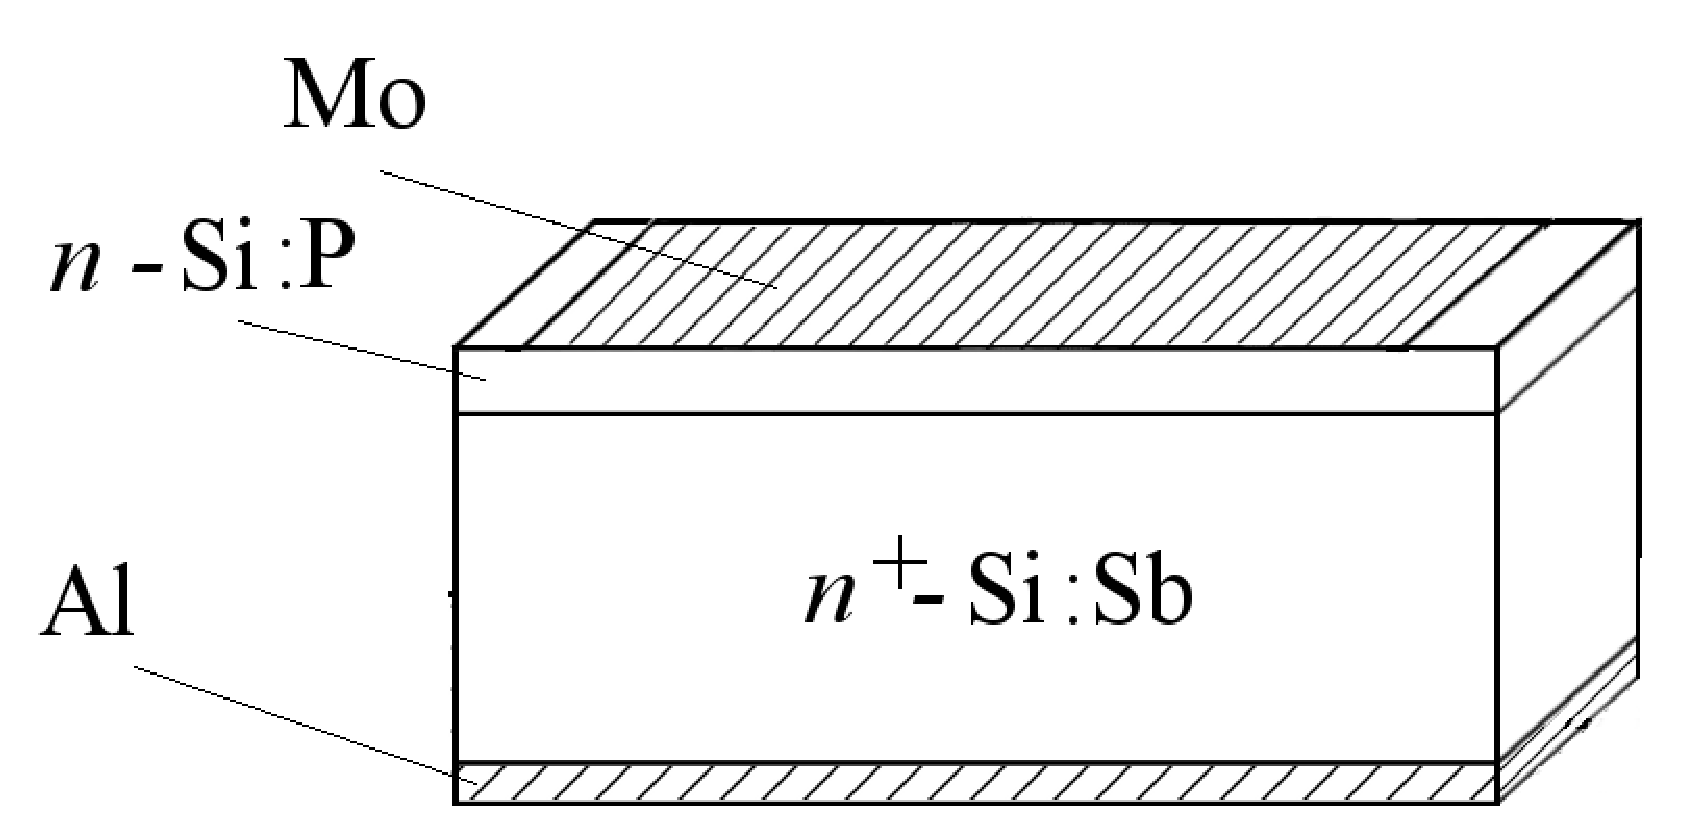
\includegraphics[width=0.6\textwidth]{MSSi2}%
\caption{\label{figMSSi2}
Структура зразків SSDB.
}
\end{figure}


В дослідженнях, результати яких представлені у цьому розділі, використовувалися діоди Шотки, виготовлені на основі епітаксійної
структури $n$--$n^+$--Si.
Товщини епітаксійного шару та підкладки дорівнювали $0,2$~мкм та $250$~мкм, відповідно.
Епітаксійний шар був легований атомами фосфору, підкладка --- сурмою
(KЭС--0.01, концентрація вільних електронів $N_s\approx4,2\cdot10^{23}$~м$^{-3}$).
Для створення бар'єру на поверхню епітаксійного прошарку нанесено шар молібдену площею $7\times7$~мм$^2$.
З протилежного боку структури нанесено прошарок алюмінію, який забезпечував наявність омічного контакту.
Схематичне зображення структур наведено на Рис.~\ref{figMSSi2}.
Структури виготовлені на <<Томилинском электронном заводе>>  (Росія).
Надалі для позначення зразків використовується скорочення SSDB.

Для контролю рівня легування епітаксійного шару були проведені
вимірювання ВФХ досліджуваних структур при кімнатній температурі.
Виявлено, що концентрація електронів в епітаксійному шарі $N_d$ становить $7\cdot10^{21}$~м$^{-3}$.

%\begin{table}
%\caption{\label{tabMSSi}Параметри структур Mo$/n$--$n^+$--Si.
%}
%%\begin{tabular}{|c|c|c|c|}
%\begin{tabularx}{\textwidth}{|>{\centering\arraybackslash}X|>{\centering\arraybackslash}X|>{\centering\arraybackslash}X|>{\centering\arraybackslash}X|>{\centering\arraybackslash}X|}
%\hline
%$N_d$, м$^{-3}$&$N_s$, м$^{-3}$&$A$, м$^2$&Позначення\\
%\hline
%$(1,1\div1,3)\cdot10^{23}$&$4,2\cdot10^{23}$&$3,14\cdot10^{-6}$&SSDA\\
%\hline
%$7,25\cdot10^{21}$&$4,2\cdot10^{22}$&$49\cdot10^{-6}$&SSDB\\
%\hline
%\end{tabularx}
%\end{table}


\section{Особливості ультразвукового навантаження при низьких температурах\label{SSDB:USL}}

Ультразвукове навантаження структур Mo$/n-n^+$--Si здійснювалось в діапазоні температур $130\div330$~К.
Схема УЗН наведена на Рис.~\ref{figUSL:SDB}.
Металевий буфер виконував роль як електричного, так і температурного екрану, ізолюючи зразок від процесів, які відбуваються у
п'єзоелектричному перетворювачі.


\begin{figure}[b]
\center
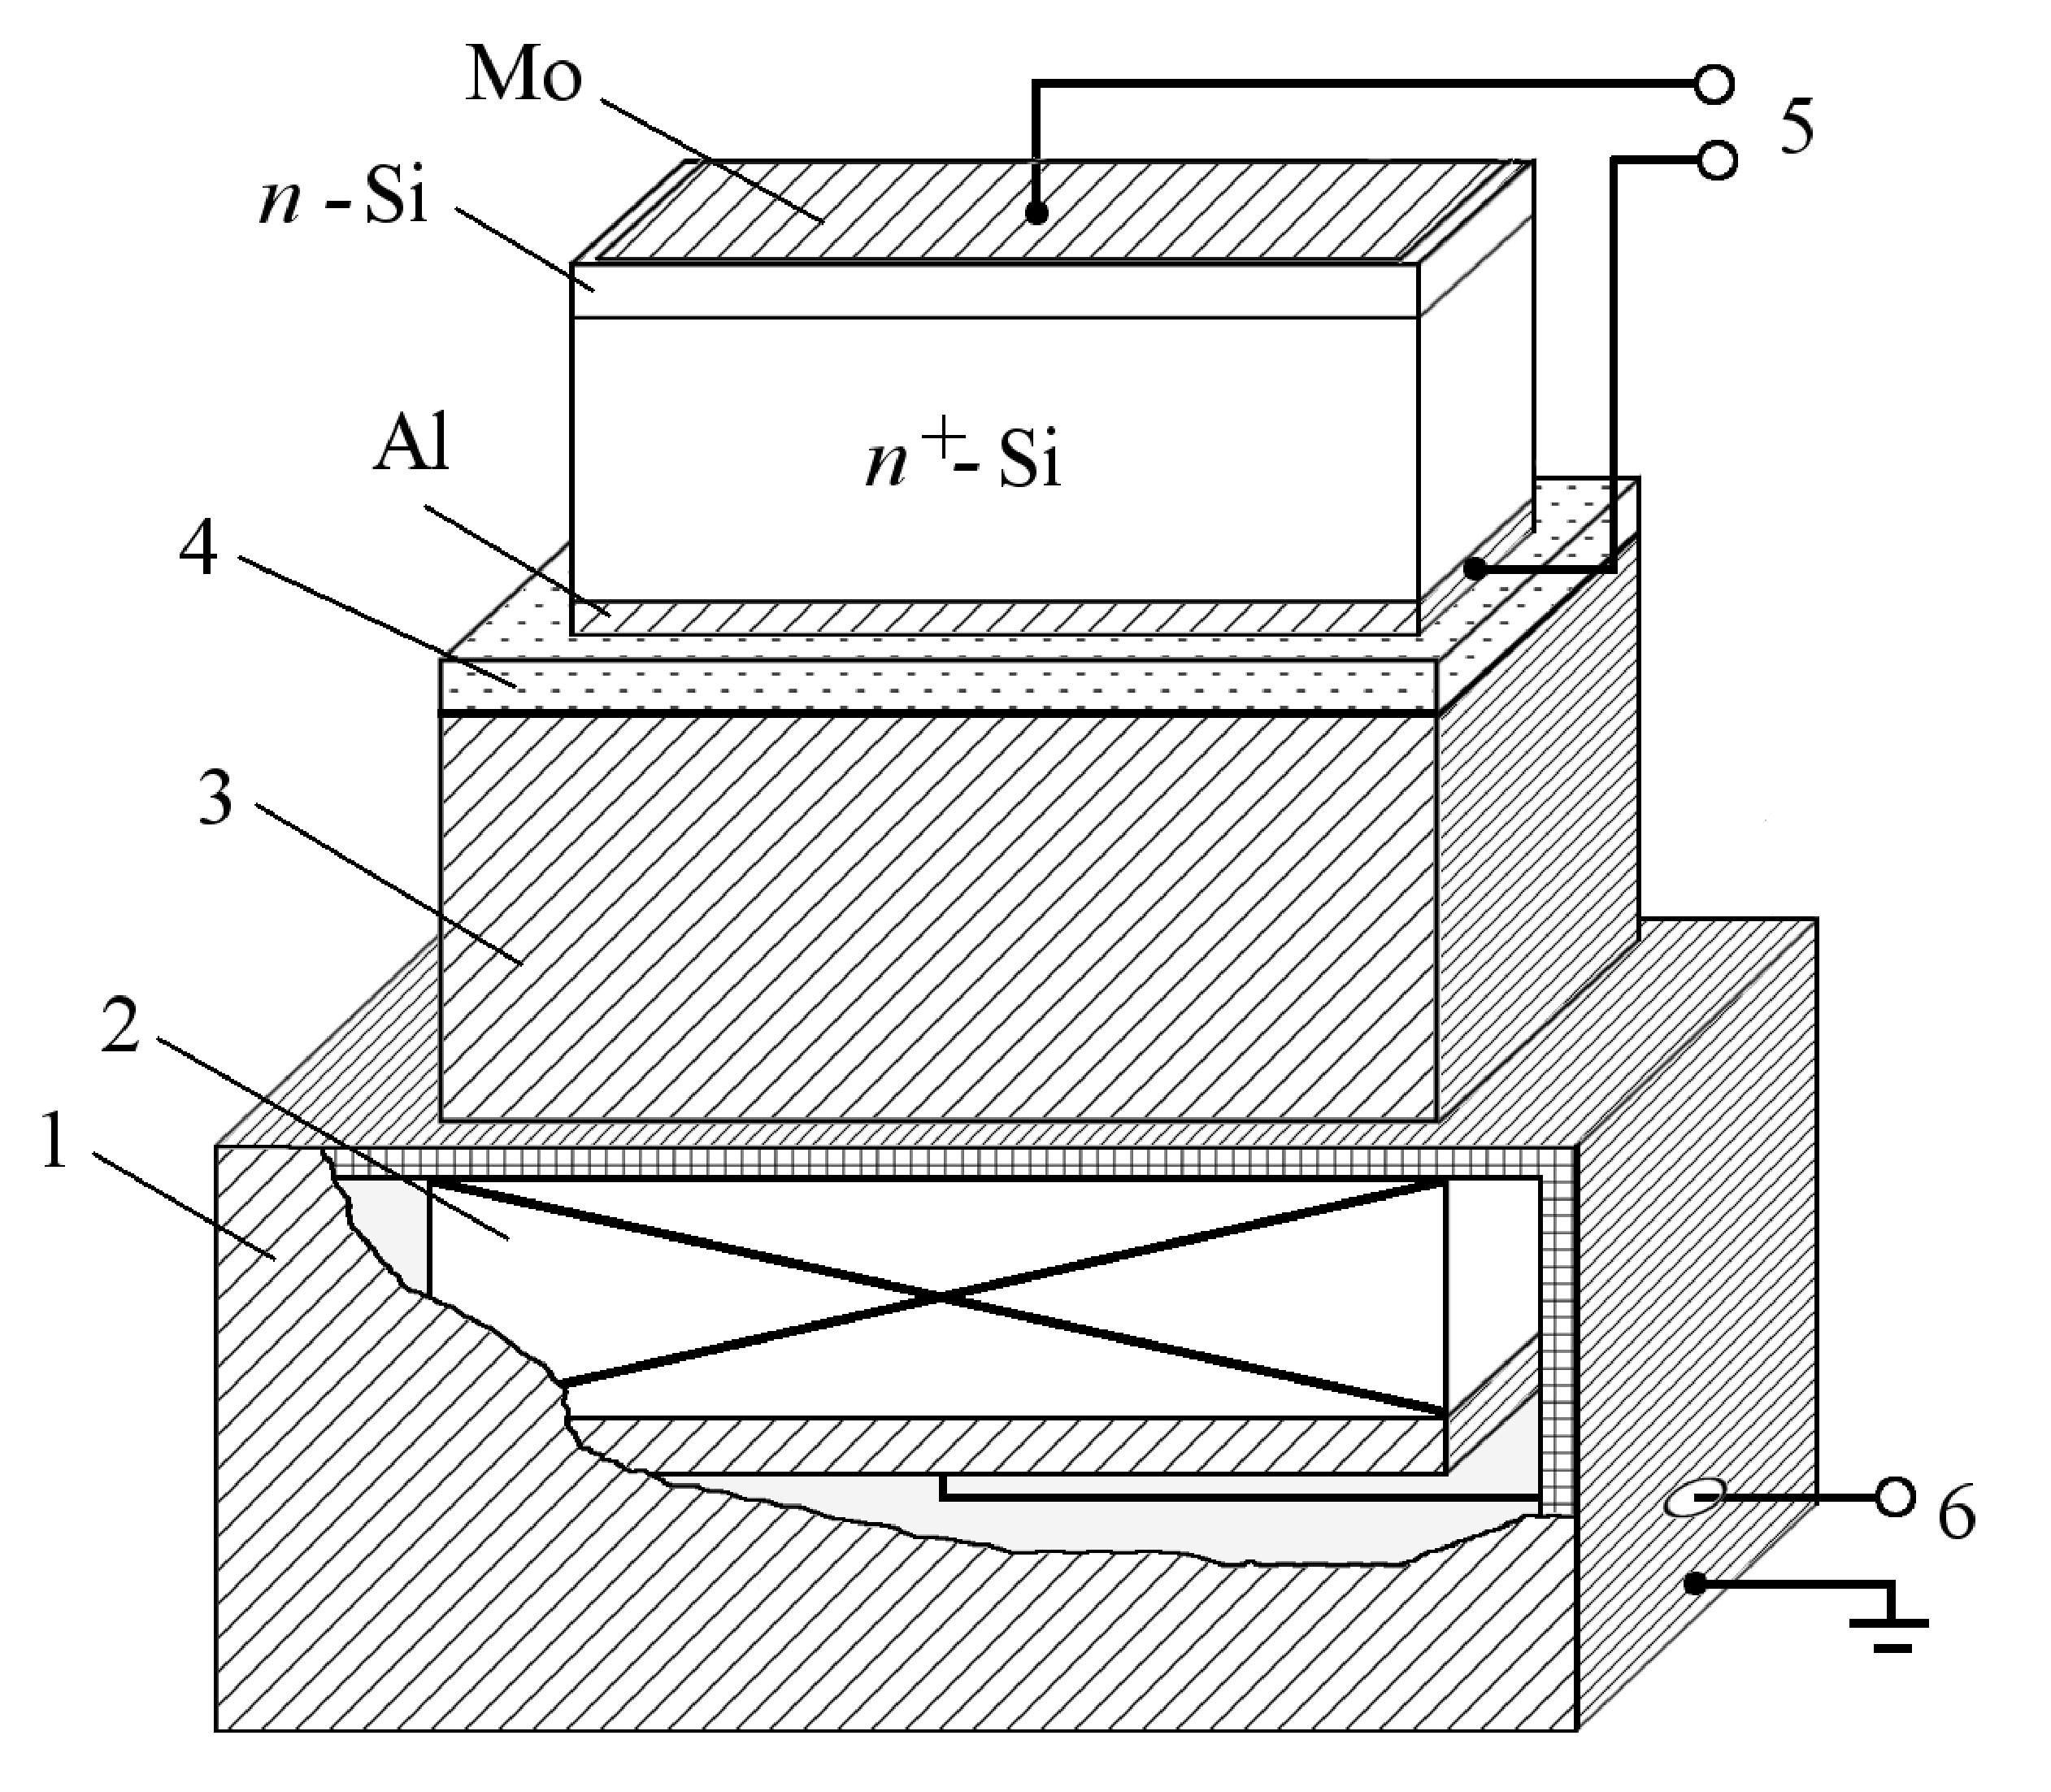
\includegraphics[width=0.5\textwidth]{USL_SDB}%
\caption{\label{figUSL:SDB}
Використані схеми УЗН.
1 --  екран (алюмінієва фольга, товщина 0,012 мм);
2 --- п'єзоелектричний перетворювач (LiNbO$_3$);
3 --- буфер (циліндр Al з високим ступенем паралельності граней, довжина 2~см);
4 --- діелектричний прошарок (слюда, товщина 0,03 мм);
5 --- контакти для вимірювання ВАХ;
6 --- контакти для збудження УЗ.
}
\end{figure}


Зауважимо, що у випадку низькотемпературного (при $T<230$~К) УЗН процес збудження АХ був утруднений через те, що
рідкі акустичні склейки на кшталт вакуумного масла кристалізувалися і переставали виконувати свою функцію.
В той же час, контакт створений при кімнатній температурі за допомогою жорсткої склейки (піцеїн або БФ6),
руйнувався при охолодженні внаслідок різниці коефіцієнтів теплового розширення.
В роботі проведення низькотемпературних УЗН при використанні повздовжніх хвиль здійснювалось за допомогою свіжого (до 5~год після нанесення) контакту з клею БФ6,
який ще не повністю кристалізувався.
Наявність акустичного контакту контролювалася за виглядом залежності повного опору перетворювача від частоти (АЧХ, амплітудно--частотної характеристики).
Зокрема, за наявності акустичного контакту на АЧХ з'являвся ряд максимумів, пов'язаних з відбиванням хвиль від граней буфера.

\begin{figure}
\center
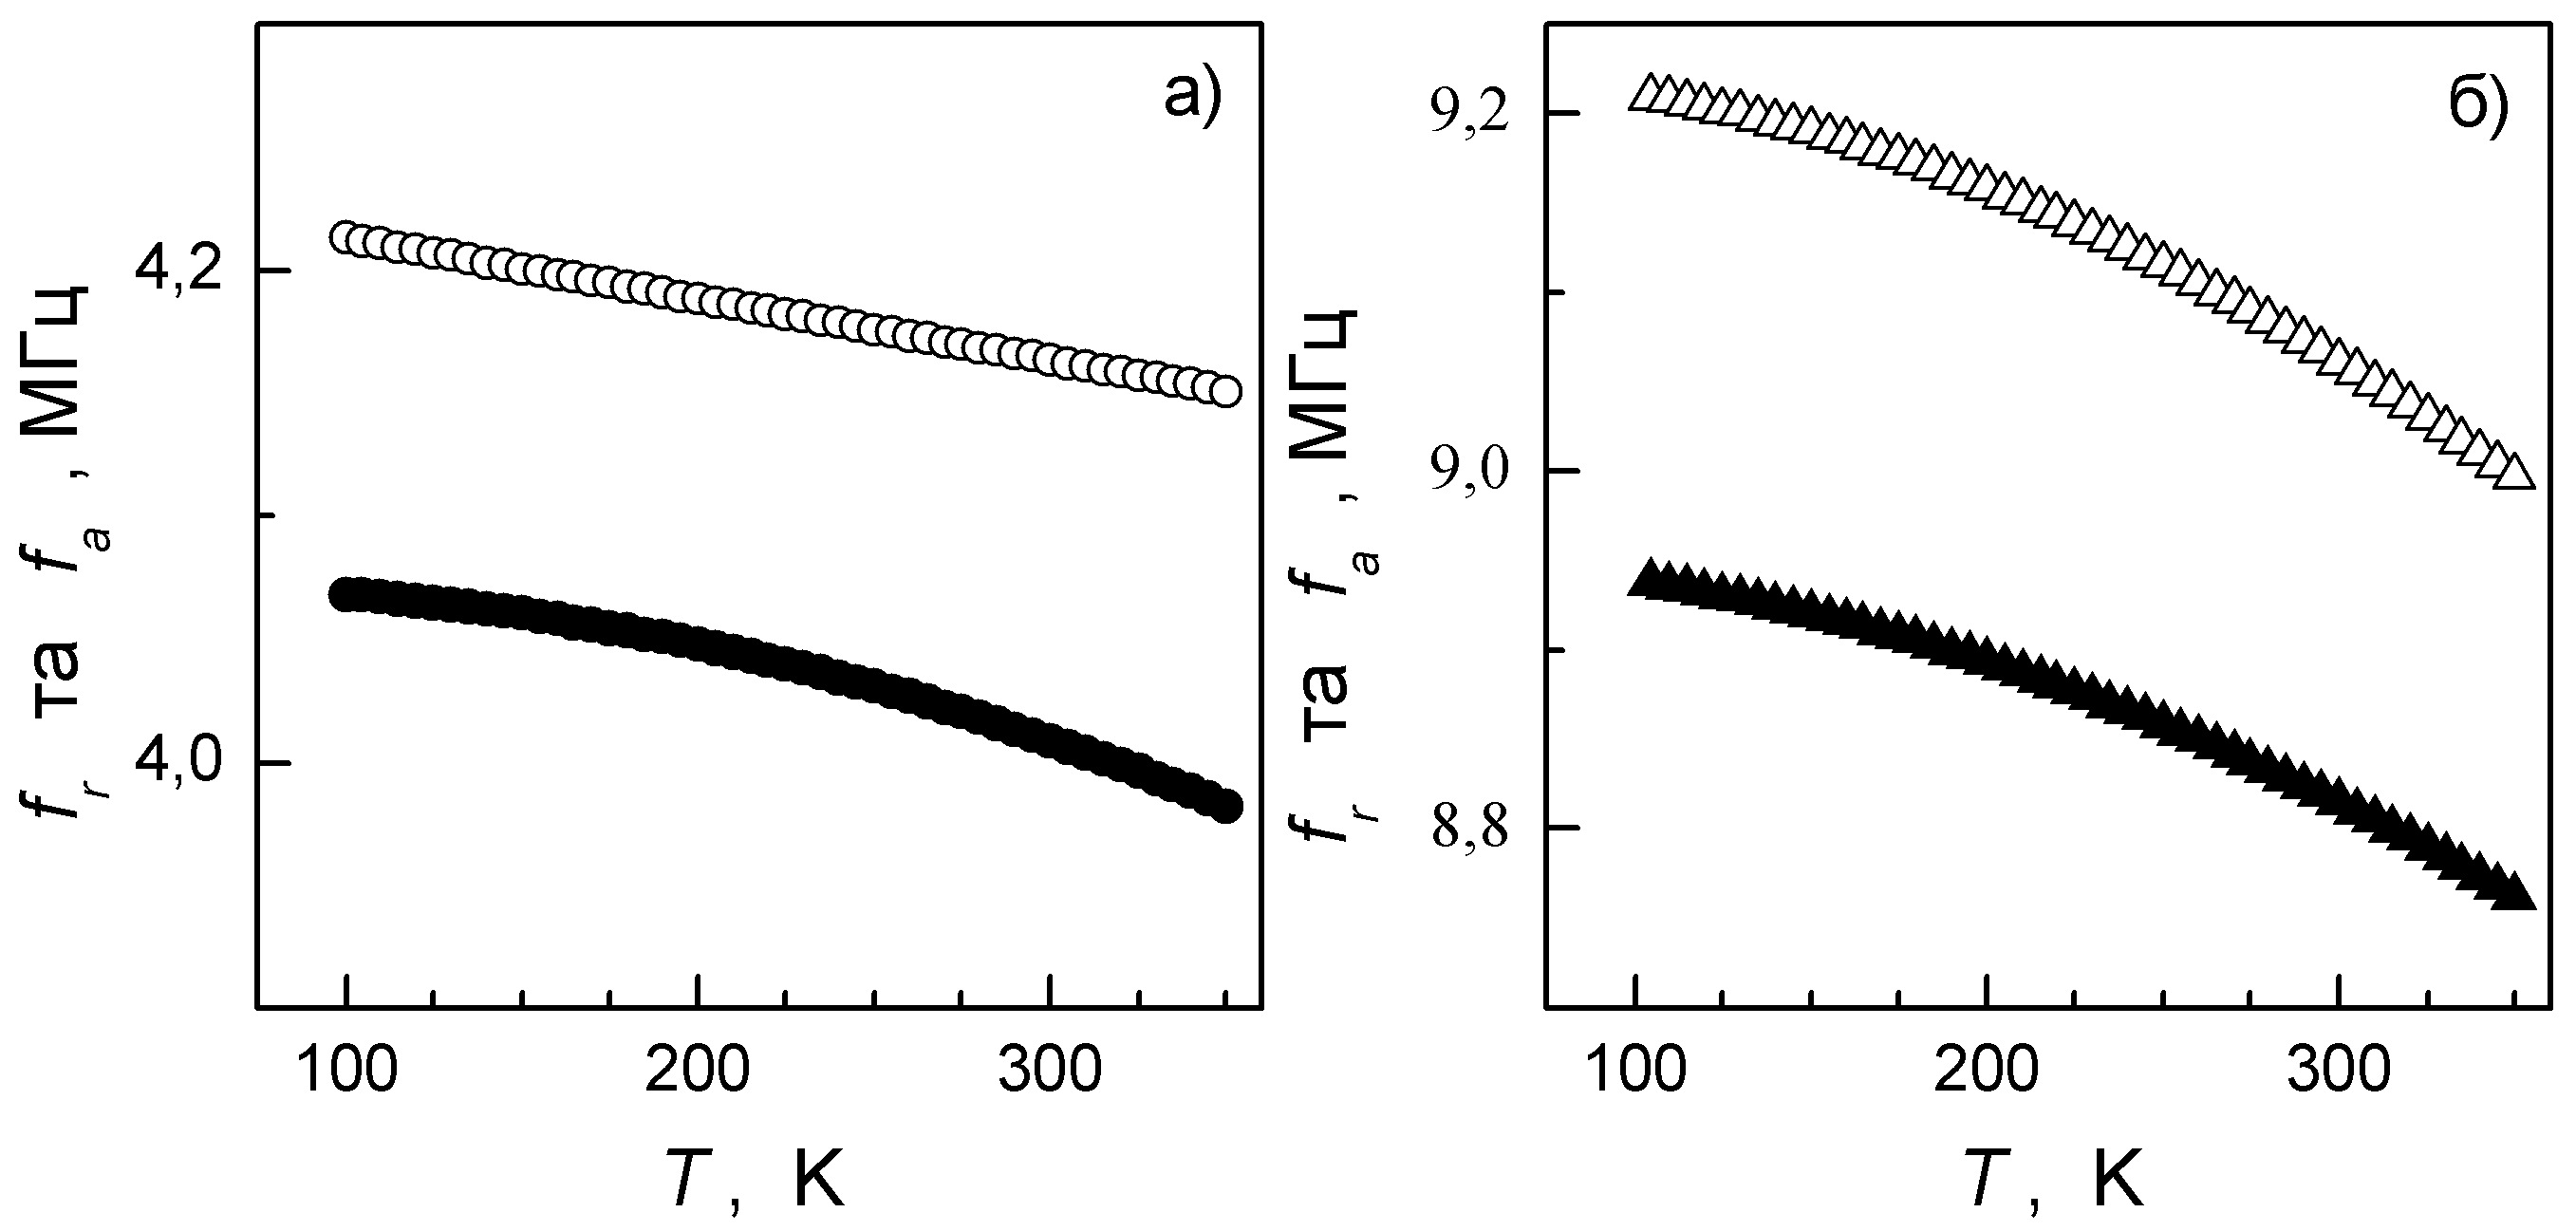
\includegraphics[width=0.7\textwidth]{figFrT}%
\caption{\label{figFrT}
Температурна залежність частот резонансу (заповнені точки) та антирезонансу (порожні точки) (перша гармоніка)
п'єзоелектричних перетворювачів LiNbO$_3$ з робочими частотами $f_\mathtt{US}$ 4,1~МГц (а) та 9,6 (б)~МГц при кімнатній температурі.
}
\end{figure}


Водночас при визначенні параметрів УЗН за допомогою формул (\labelcref{eqAmpUS,eqWus,eqM0,eqDefUS}) та даних Таблиці~\ref{tabLNO} викликає ряд труднощів.
По--перше, параметри матеріалу є температурозалежними.
Наприклад, з літератури відомо, що зміна пружних сталих при збільшенні температури на 100 К для LiNbO3 становить приблизно (-2\%) \cite{LNO_C:Temp},
а для кремнію --- (-2.5\%) \cite{Si_C:Temp};
типові температурні залежності резонансної та антирезонансної частот показані на Рис.~\ref{figFrT}.
При дослідженні АІ ефектів в структурах SSDB вимірювання проводилися в достатньо широкому температурному інтервалі і тому подібними залежностями нехтувати не можна.
По--друге, наявність буфера була причиною втрат акустичної енергії внаслідок поглинання УЗ в алюмінієвому циліндрі, часткового відбивання пружних хвиль
при переході з одного середовища в інше, тощо.
Ці ефекти також не враховані у виразах (\ref{eqWus}) і  (\ref{eqM0}).



Враховуючи зазначене вище, оцінка інтенсивності введеного у зразок УЗ здійснювалася за допомогою виразу
 \begin{equation}
 \label{eqWus2}
 W_\mathtt{US}=\frac{V_\mathtt{RF}^2}{2\,A_\mathtt{LNO}\,Z_\mathtt{LNO}}\,K_\mathtt{LNO}^2\,l_\mathtt{US},
 \end{equation}
де
$Z_\mathtt{LNO}$ --- імпеданс акусто--навантаженого перетворювача,
$l_\mathtt{US}$ --- коефіцієнт, який враховує загальні втрати пружної енергії.
При цьому вважалося, що величини
$K_\mathtt{LNO}$, $Z_\mathtt{LNO}$ та $l_\mathtt{US}$ залежать від температури.

Визначення $K_\mathtt{LNO}$ та $l_\mathtt{US}$ відбувалося з використанням стандартної схеми,
зображеної на Рис.~\ref{Luna2},а.
В системі збуджувалися імпульси УЗ за допомогою одного з ідентичних п'єзоперетворювачів і реєструвалися
високочастотні сигнали на другому.
Амплітуди сигналів $V_\mathtt{RF}^{(1)}$ та $V_\mathtt{RF}^{(2)}$, пов'язаних з однократним та троєкратний (після відбиття від правої та лівої границь) проходженням акустичного імпульсу через систему
(див. Рис.~\ref{Luna2},б) можуть бути записані у вигляді
 \begin{equation}
 \label{eqVrf1}
 (V_\mathtt{RF}^{(1)})^2=V_\mathtt{RF}^2\,K_\mathtt{LNO}^4\,l_\mathtt{US},
 \end{equation}
 \begin{equation}
 \label{eqVrf2}
 (V_\mathtt{RF}^{(2)})^2=V_\mathtt{RF}^2\,K_\mathtt{LNO}^4\,l_\mathtt{US}^3.
 \end{equation}

\begin{figure}
\center
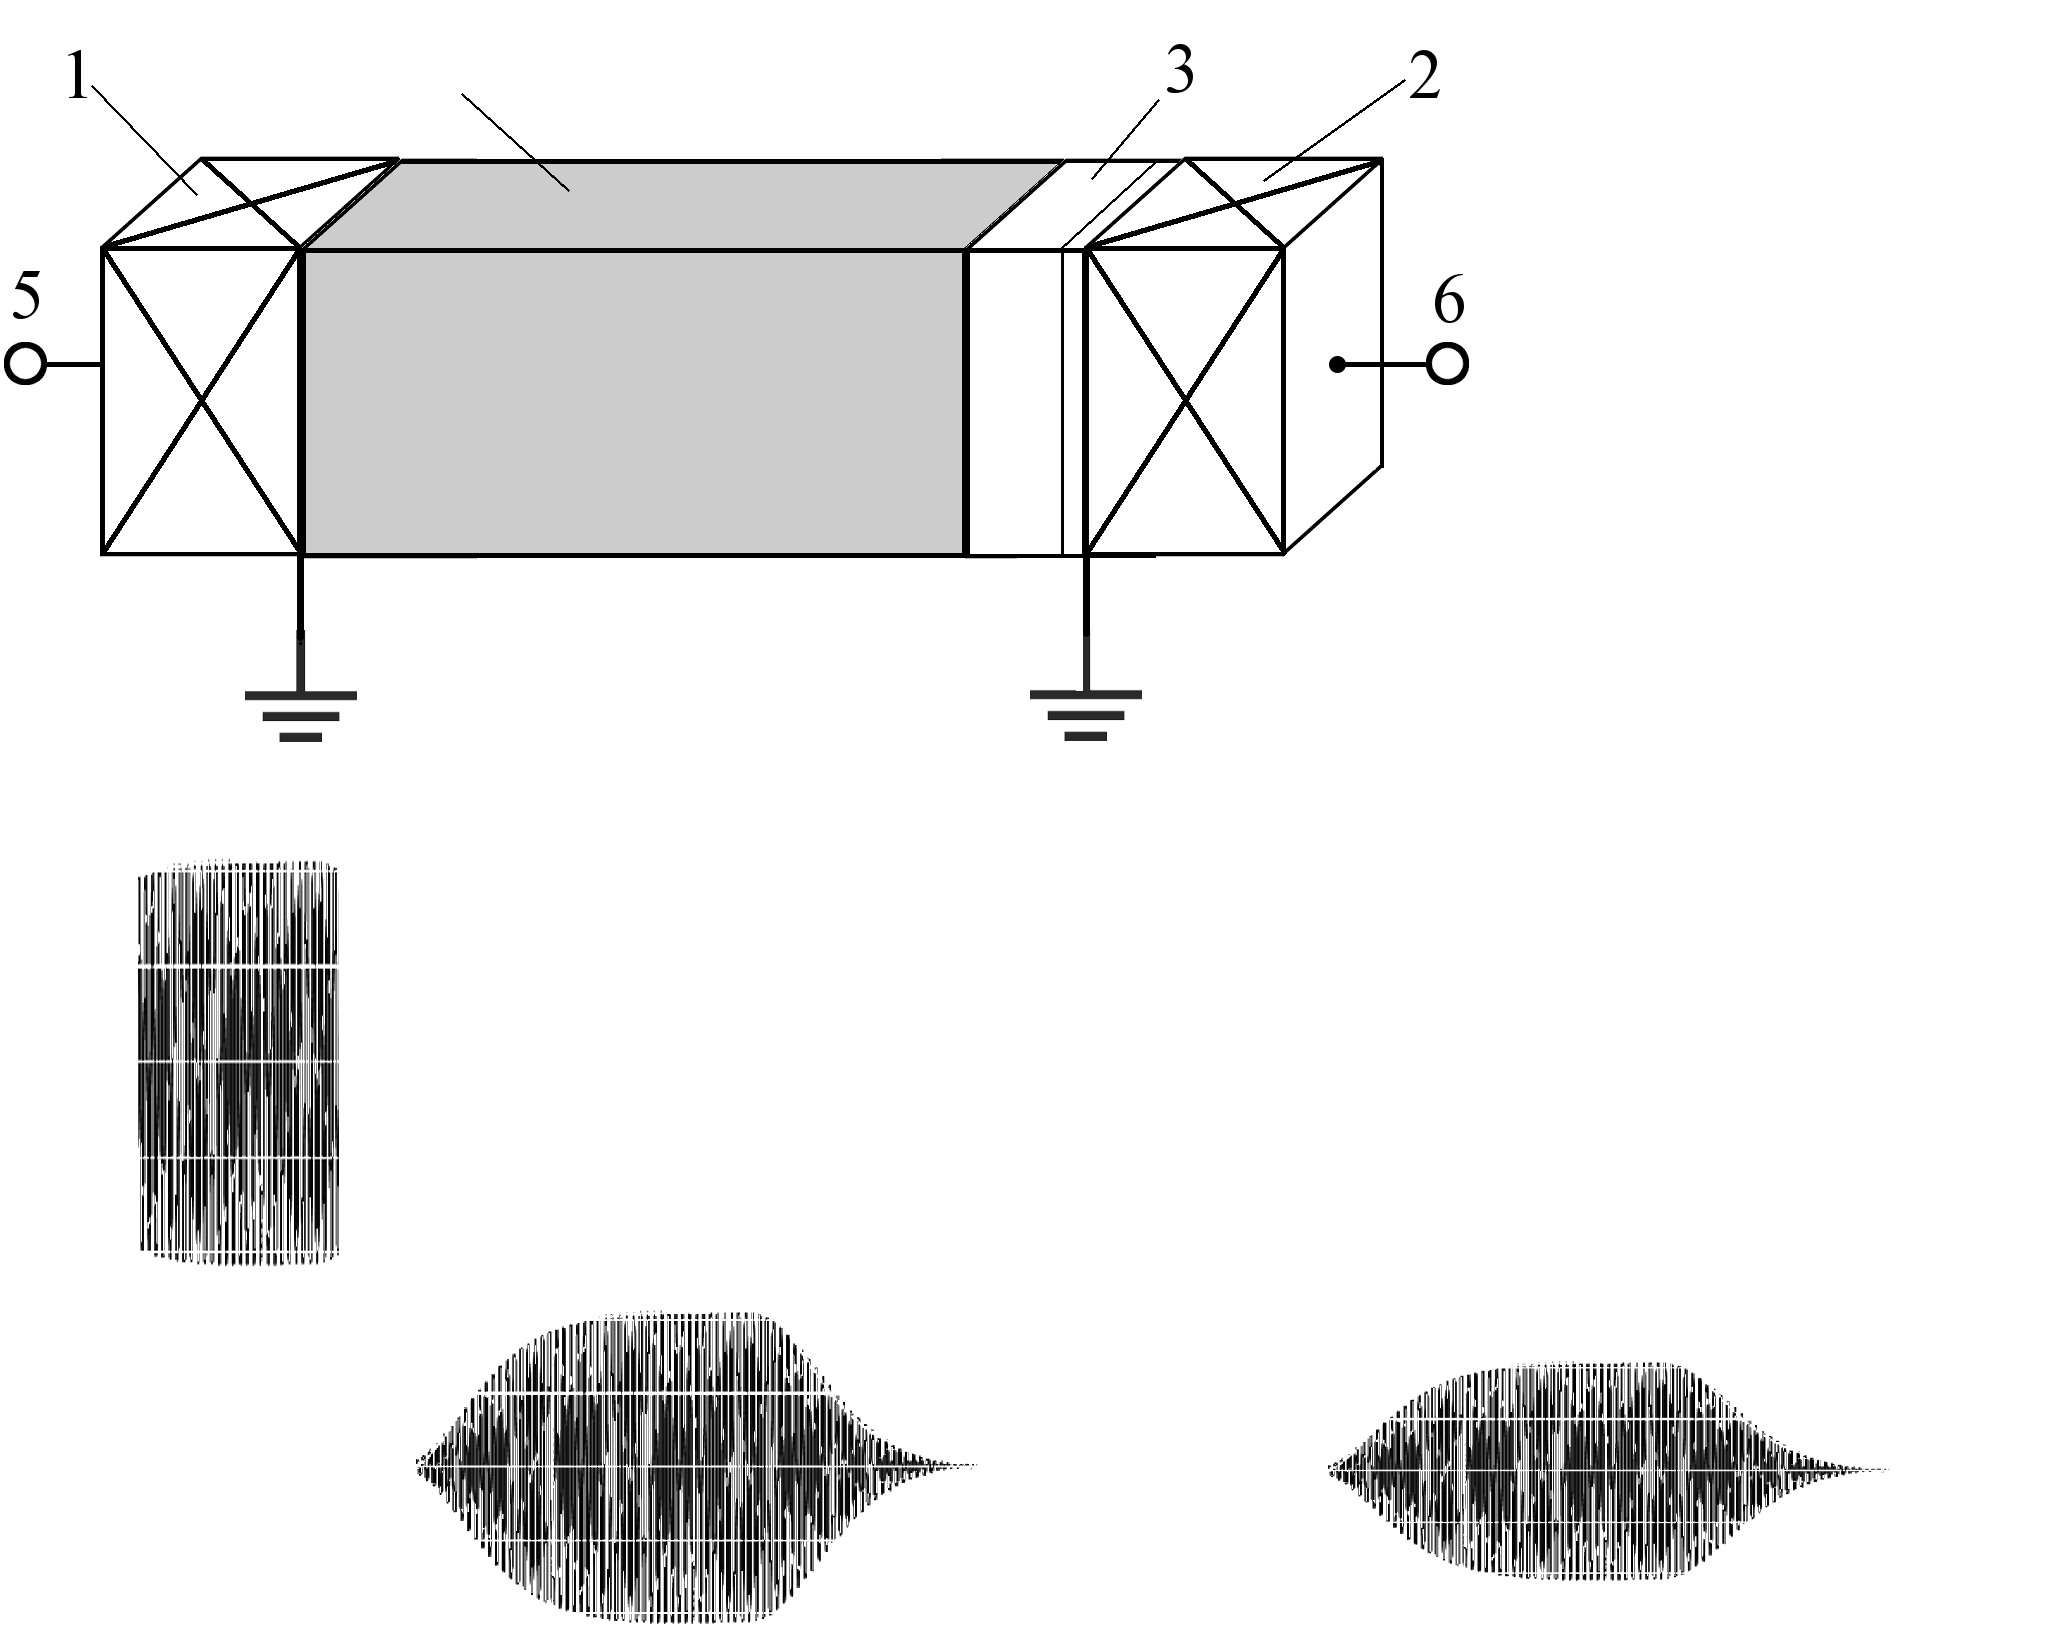
\includegraphics[width=0.9\textwidth]{Luna2}%
\caption{\label{Luna2}
а: Схема для оцінки інтенсивності введеного УЗ.
1, 2 --- ідентичні п'єзоелектричні перетворювачі,
3 --- SSDB,
4 --- буфер (Al),
5, 6 --- електроди збуджуючого та приймаючого перетворювачів, відповідно.
б: Схематична осцилограма сигналів на електродах п'єзоперетворювачів.
в: Схема для визначення імпедансу п'єзоперетворювача.
7 --- датчик струму,
8 --- еталонний опір.
}
\end{figure}

Останні два співвідношення дозволяють визначити акустичні параметри системи на основі вимірювання амплітуд
високочастотних сигналів на електродах збуджуючого та приймаючого п'єзоперетворювачів.
Приклад отриманих температурних залежностей для однієї частоти наведено на Рис.~\ref{figKp2T},а та Рис.~\ref{figKp2T},б.

\begin{figure}
\center
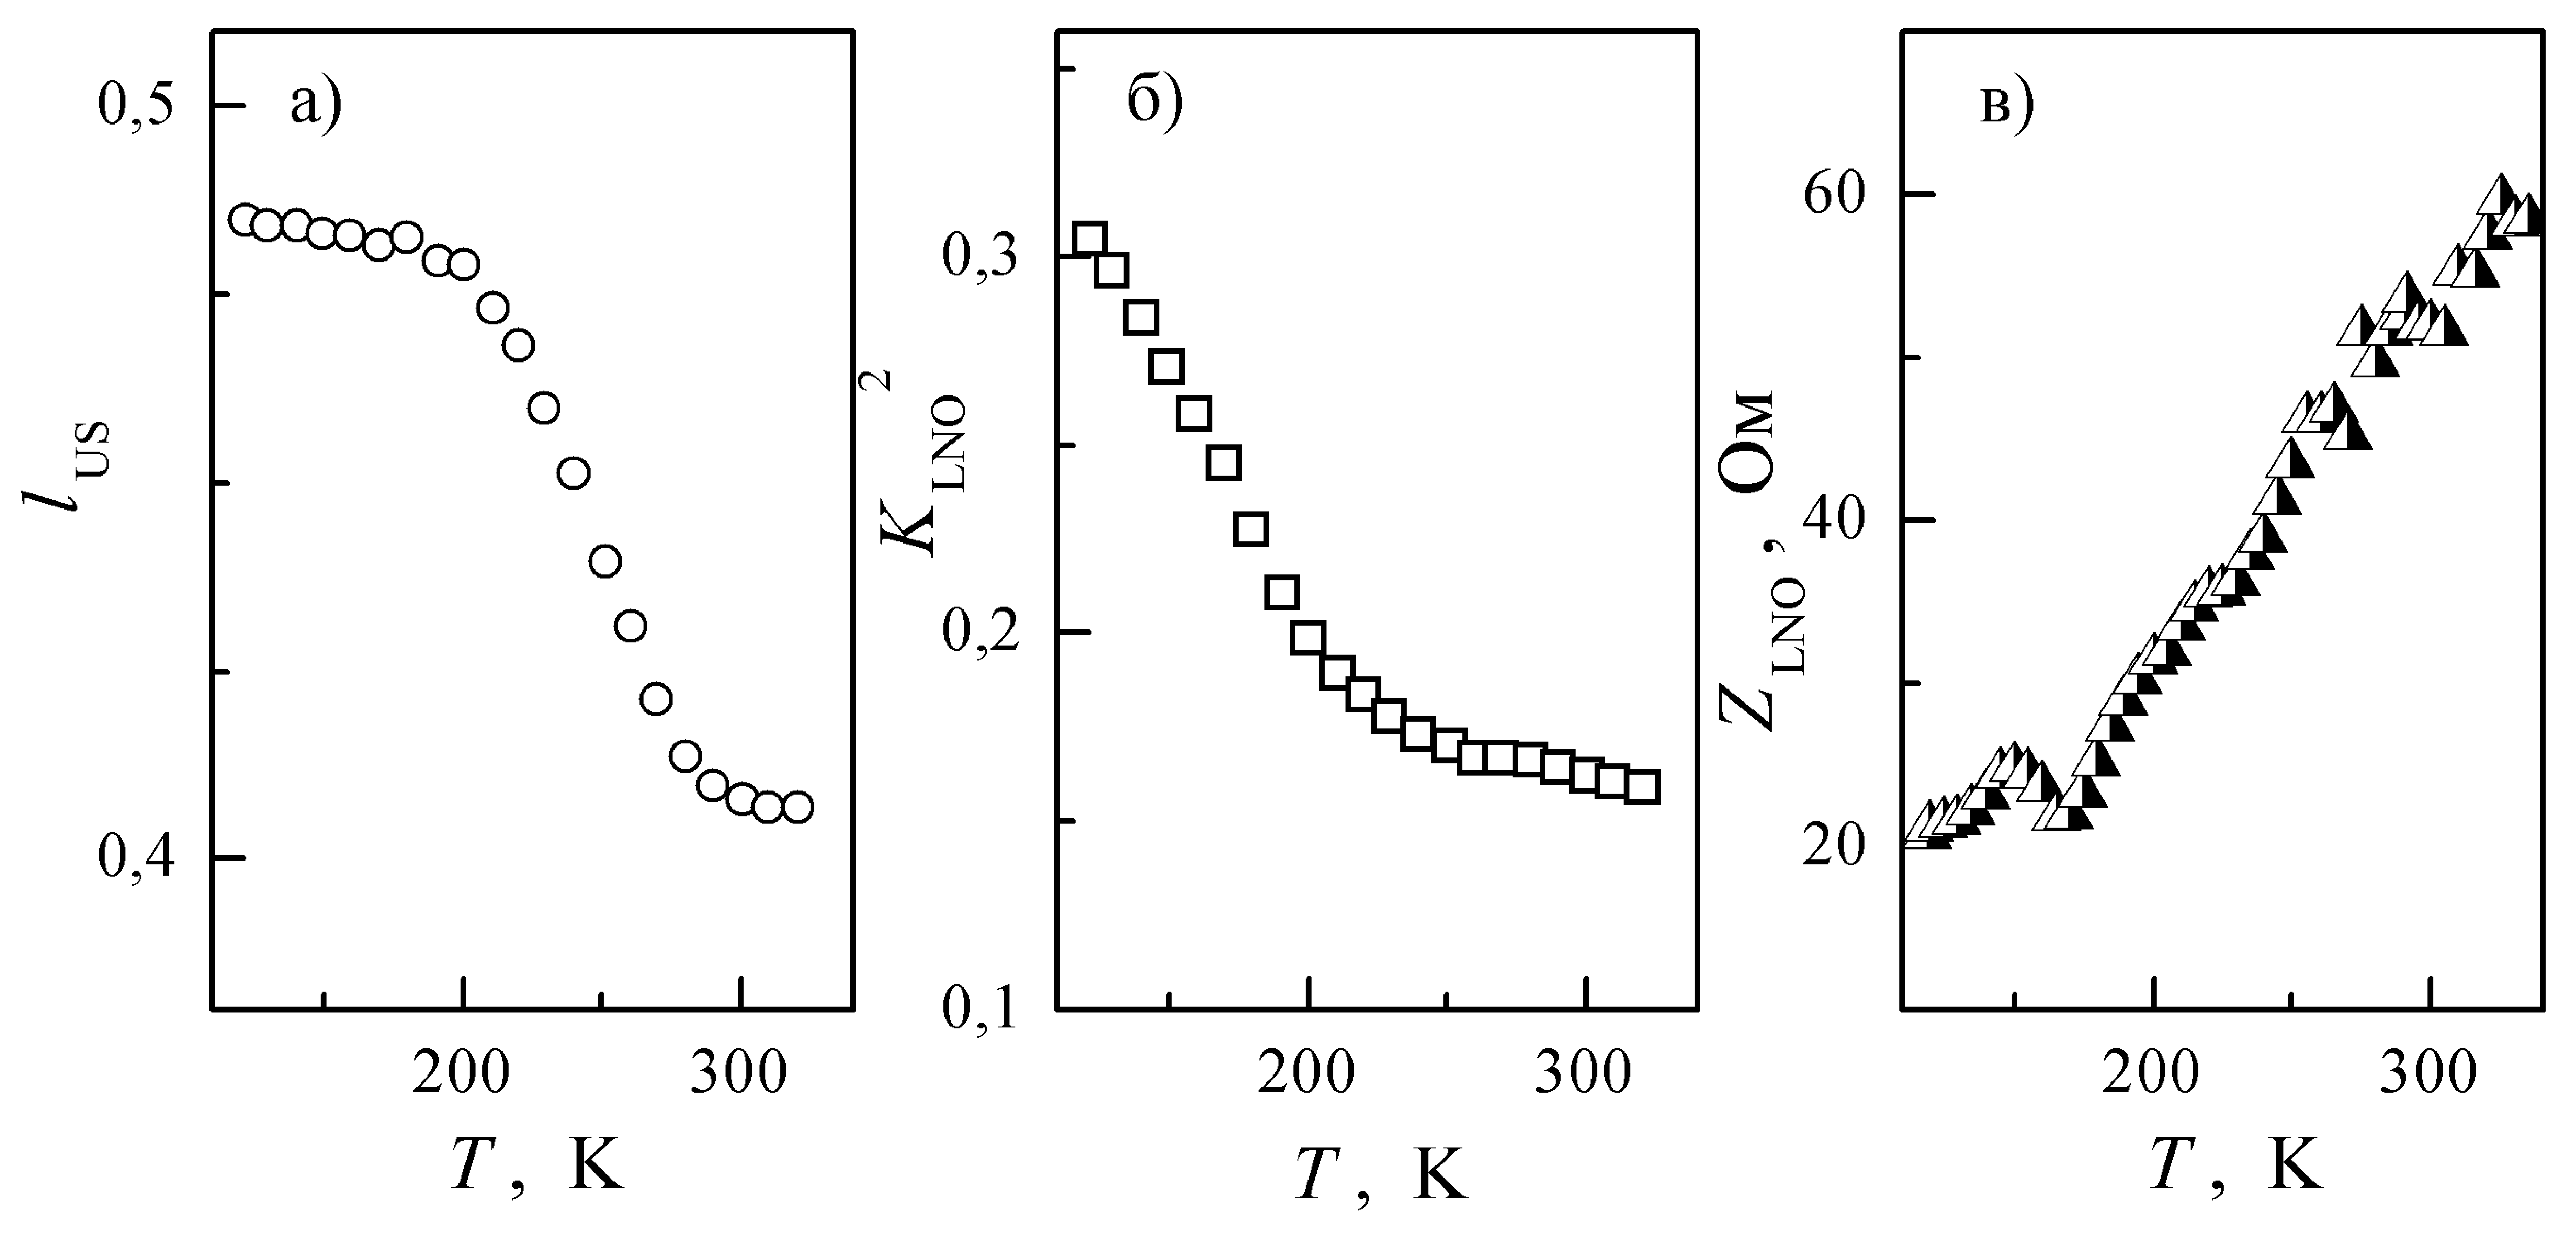
\includegraphics[width=0.9\textwidth]{figKp2T}%
\caption{\label{figKp2T}
Температурні залежності коефіцієнта акустичних втрат (а),
квадрата коефіцієнта електромеханічного зв'язку (б) та
імпедансу (в) п'єзоперетворювача з робочою частотою $f_\mathtt{US}=8,4$~МГц.
}
\end{figure}

Для оцінки $Z_\mathtt{LNO}$ використовувався метод,
схема якого представлена на Рис.~\ref{Luna2},в.
Датчиком струму слугувало феритове кільце із дротяною обмоткою.
Кількість витків обмотки підбиралось для кожної частоти таким чином, щоб для випадку, коли під'єднано еталонний опір $R_\mathtt{st}$,
зсув фаз між збуджуючим сигналом амплітудою $V_\mathtt{RF,st}$ та сигналом з датчика амплітудою $V_\mathtt{L,st}$
дорівнював нулеві.
Величина імпедансу розраховувалася за допомогою виразу
 \begin{equation}
 \label{eqZlno}
 Z_\mathtt{LNO}=\frac{V_\mathtt{RF}}{V_\mathtt{L}}\,\frac{V_\mathtt{L,st}}{V_\mathtt{RF,st}}\,R_\mathtt{st}.
 \end{equation}

В роботі використовувався еталонний опір величиною 56,7~Ом.
Температурна залежність імпедансу одного з перетворювачів наведена на Рис.~\ref{figKp2T},в.

Використання виразу (\ref{eqWus2}) та даних Рис.~\ref{figKp2T} показує, що при подачі на електроди п'єзоелектричного перетворювача
високочастотної напруги з постійною амплітудою в діапазоні температур $130\div330$ призводить до поширення у зразку АХ з
інтенсивністю, яка змінюється більше ніж в п'ять разів --- Рис.~\ref{figWusT},а.
З іншого боку, поблизу кімнатних температур наближення, яке використовувалося у розділі \ref{Ch_SSC}, про те, що сталому значенню
$V_\mathtt{RF}$ відповідає постійна величина $ W_\mathtt{US}$, справедливе з точністю до 10 відсотків.
На Рис.~\ref{figWusT},б також показано як має змінюватись амплітуда напруги на п'єзоперетворювачі, щоб при різних температурах
інтенсивність УЗН залишалась постійною.


\begin{figure}
\center
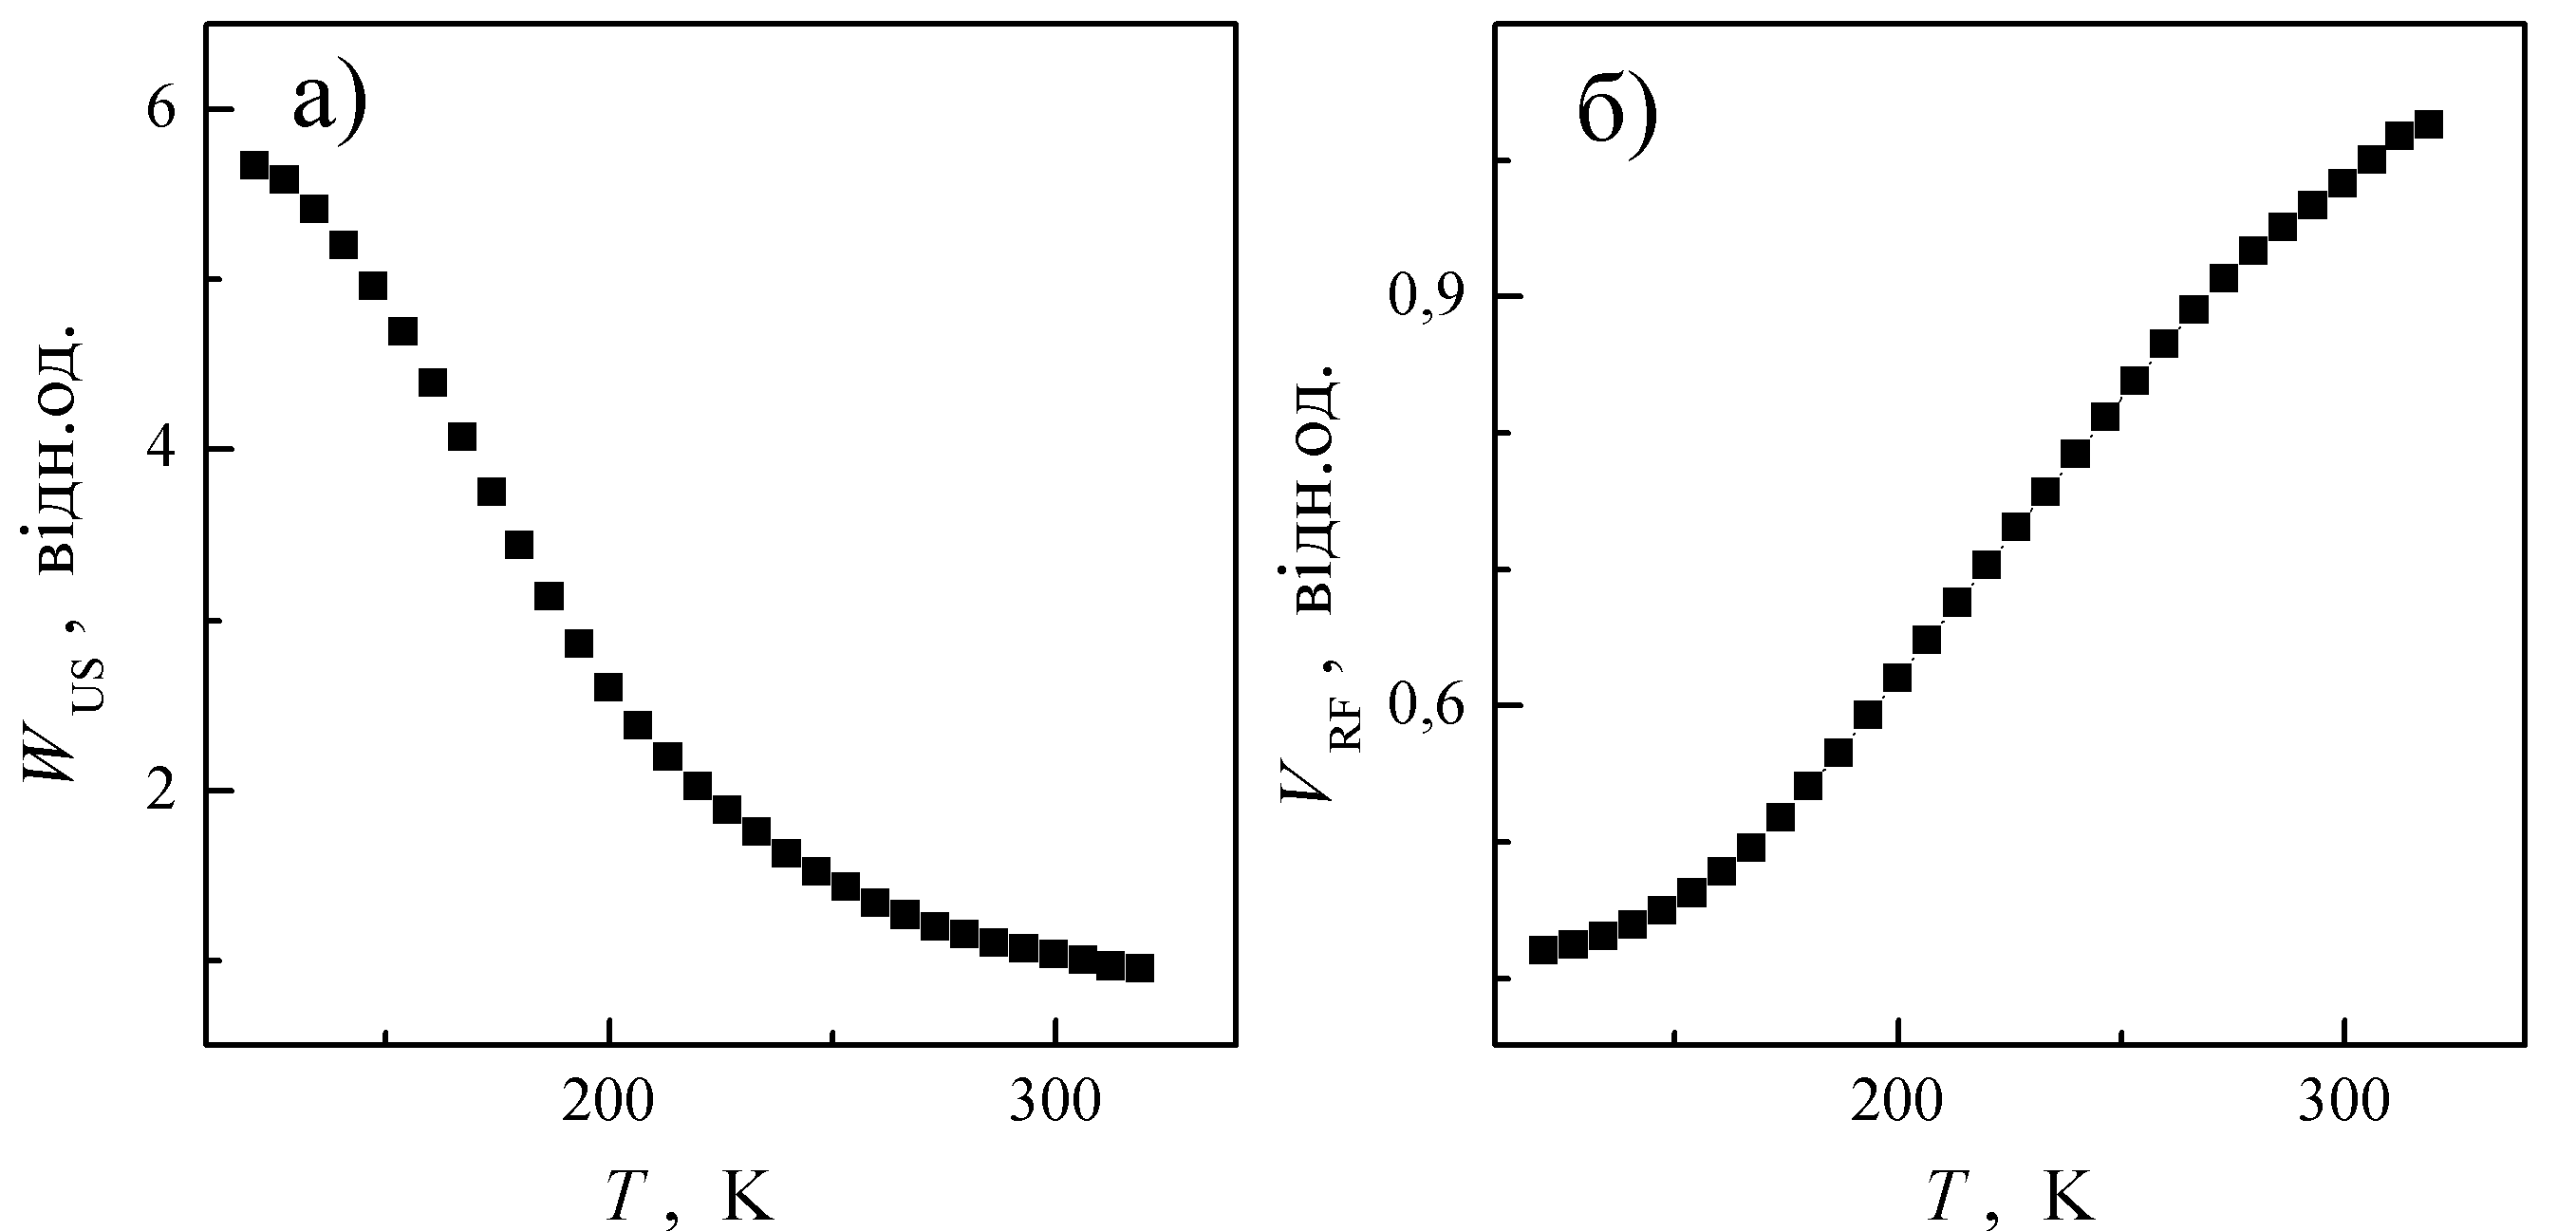
\includegraphics[width=0.9\textwidth]{figWusT}%
\caption{\label{figWusT}
Температурні залежності
інтенсивності введеного УЗ при постійному значенні амплітуди напруги на п'єзоперетворювачі (а)
та необхідної амплітуди на п'єзоперетворювачі для постійності інтенсивності введеного УЗ (б)
для п'єзоперетворювача з робочою частотою $f_\mathtt{US}=8,4$~МГц.
}
\end{figure}

У роботі збудження повздовжніх АХ в структурах SSDB відбувалося на частотах 4,1, 8,4 та 27,8 МГц.
Виміри проводилися як при сталому значенні $V_\mathtt{RF}$ при різних температурах, так і при постійній інтенсивності введеного УЗ.
Для позначення сімейства УЗН з $f_\mathtt{US}=4,1$~МГц надалі використовується скорочення U4SDB.
Аналогічні за змістом скорочення U8SDB та U28SDB застосовуються і до інших сімейств.
Для кожної з частот бути проведені калібрувальні виміри, структура яких описана вище, і побудовані градуювальні характеристики,
аналогічні представленим на Рис.~\ref{figWusT}.





\section{Динамічні ефекти впливу ультразвуку на \emph{I--V--T} характеристики кремнієвих структур з бар'єром Шотки\label{SSDB:Forw}}

\begin{figure}
\center
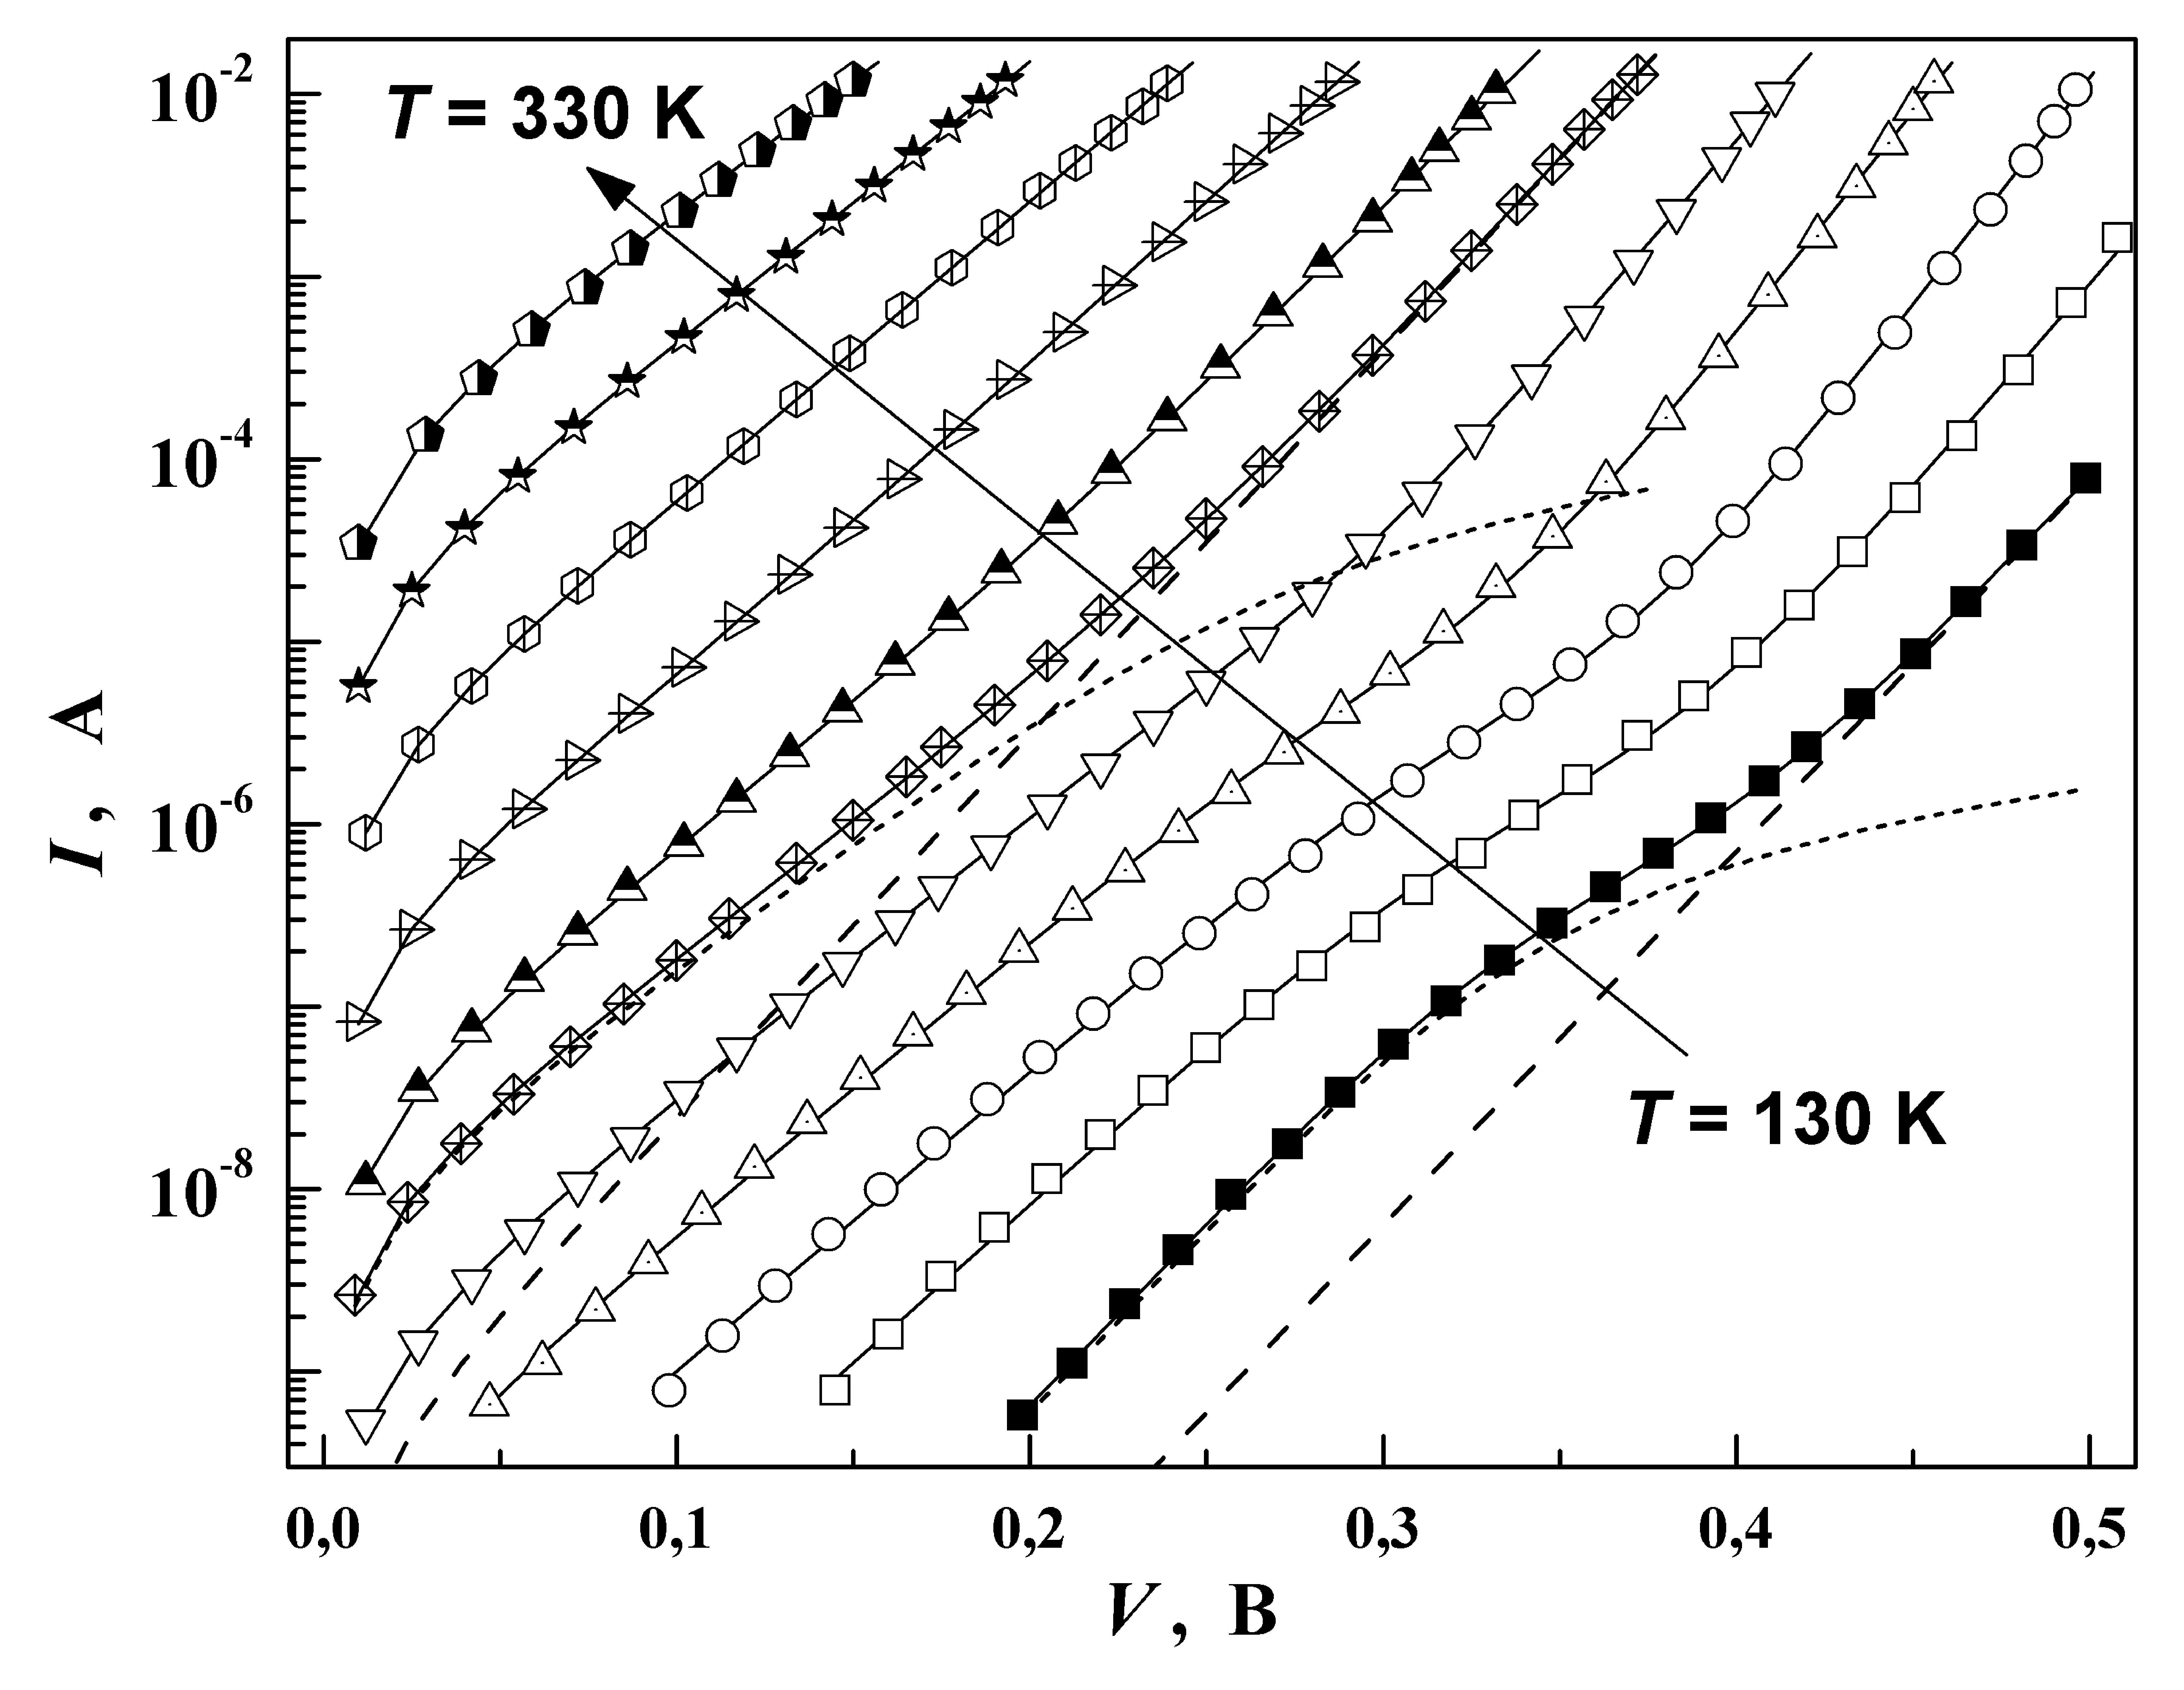
\includegraphics[width=0.8\textwidth]{figIV_SDB}
\caption{\label{figIV_SDB}
Прямі  ділянки ВАХ структур Mo/$n$--Si з контактом Шотки в температурному діапазоні $130\div330$~К.
Наведено криві, виміряні з кроком 20~К.
Точки --- експеримент,
суцільні лінії --- апроксимація за формулою~(\ref{eqSDB_IV}).
Штрихові та пунктирні лінії --- ВТКС та НТКС, відповідно.
}%
\end{figure}


Набір прямих ВАХ структур  SSDB, виміряних при різних температурах без УЗН, представлений на Рис.~\ref{figIV_SDB}.
Загалом, ВАХ схожі, на характеристики структур SSDA:
при зниженні температури та малих зміщеннях суттєвим стає внесок додаткової компоненти прямого струму, причому
на вигляд відповідної ділянки ВАХ значний внесок має послідовний опір.
В той же час при високих температурах ВАХ в напівлогарифмічному масштабі близька до лінійної.
Враховуючи ці особливості, для апроксимації ВАХ використовувався наступний вираз:
\begin{equation}
\label{eqSDB_IV}
  I=I_H+I_L=I_{s,H}\left[\exp\left(\frac{qV}{n_\mathrm{id,H}kT}\right)-1\right]+
 I_{s,L}\left\{\exp\left[\frac{q(V-IR_S)}{n_\mathrm{id,L}kT}\right]-1\right\},
\end{equation}
де
$I_H$ та $I_L$ --- ВТКС та НТКС, відповідно;
$I_{s,H}$ та $I_{s,L}$ --- струми насичення компонент,
$n_{H}$ та $n_{L}$ --- ідеальні фактори.
Апроксимація здійснювалась за допомогою методу штучної бджолиної сім'ї,
як шукані параметри розглядалися $I_{s,H}$, $I_{s,L}$, $n_{H}$, $n_{L}$ та $R_s$.
Зауважимо, що MABC використовувався для будь-якої нелінійної апроксимації, яка згадується у частині~\ref{SSDB:Forw}.
Результати апроксимації прямих ВАХ також показані на Рис.~\ref{figIV_SDB}.
Видно, що відхилення апроксимуючих кривих від експериментально отриманих точок мінімальне
(коефіцієнт кореляції більше 0,99).

\begin{figure}
\center
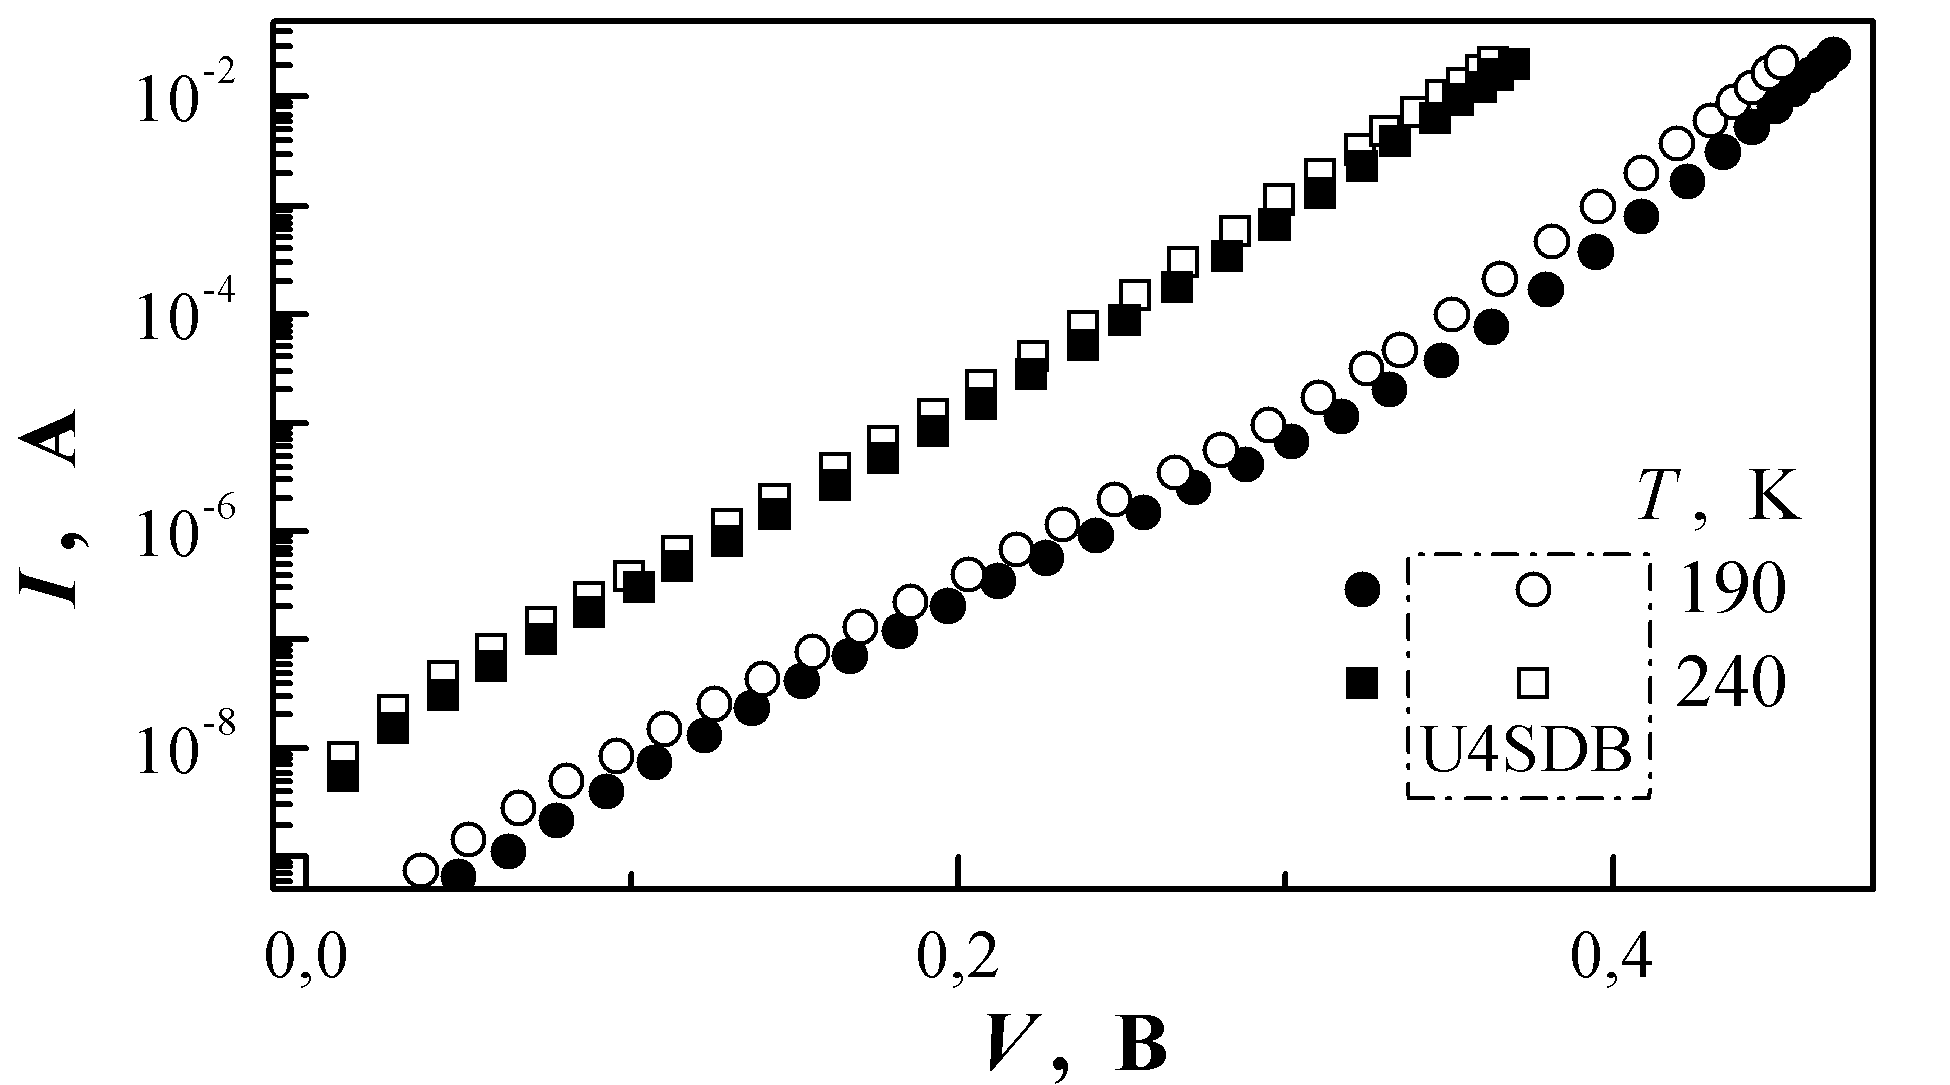
\includegraphics[width=0.8\textwidth]{figIVUS_SDB}
\caption{\label{figIVUS_SDB}
Приклади ВАХ структур SSDB, виміряних при однаковій температурі в умовах U8SDB (порожні точки) та без нього (заповнені точки).
$T$, К: 190 (кола), 240 (квадрати).
}%
\end{figure}

За умов УЗН, температурна та польова залежності прямого струму схожі,
проте спостерігається збільшення величини $I$ --- див. Рис.~\ref{figIVUS_SDB}.
Нижче окремо розглянуто вплив УЗН на кожну з компонент струму.


\subsection{Параметри високо--температурної компоненти струму}

Обчислення висоти бар'єру Шотки здійснювалось в наближенні теорії ТЕ за допомогою формули~(\ref{eqFb:TE}).
Температурна залежність ВБШ для високотемпературної компоненти струму ВТКС представлена на Рис.~\ref{figFbH_SDB}.
На рисунку показані результати, отримані для акустично ненавантаженого зразка,
а також приклад залежності, розрахованої для випадку УЗН з частотою $4,1$~МГц.
Видно, що при поширенні УЗ в структурі, висота бар'єру змінюється,
причому як величина, так і знак змін залежать від температури.
Залежності АІ змін $\Phi_{b}$ наведено на Рис.~\ref{figDelFbH}.
Зазначимо, згідно з прийнятими позначеннями (див. формулу~(\ref{eqAbsDelta})),
від'ємне значення $\Delta \Phi_{b,H}$ відповідає збільшенню висоти бар'єру за умов дії УЗ і тому
додатній напрямок вертикальної осі на Рис.~\ref{figDelFbH} для зручності спрямовано вниз.



\begin{figure}
\center
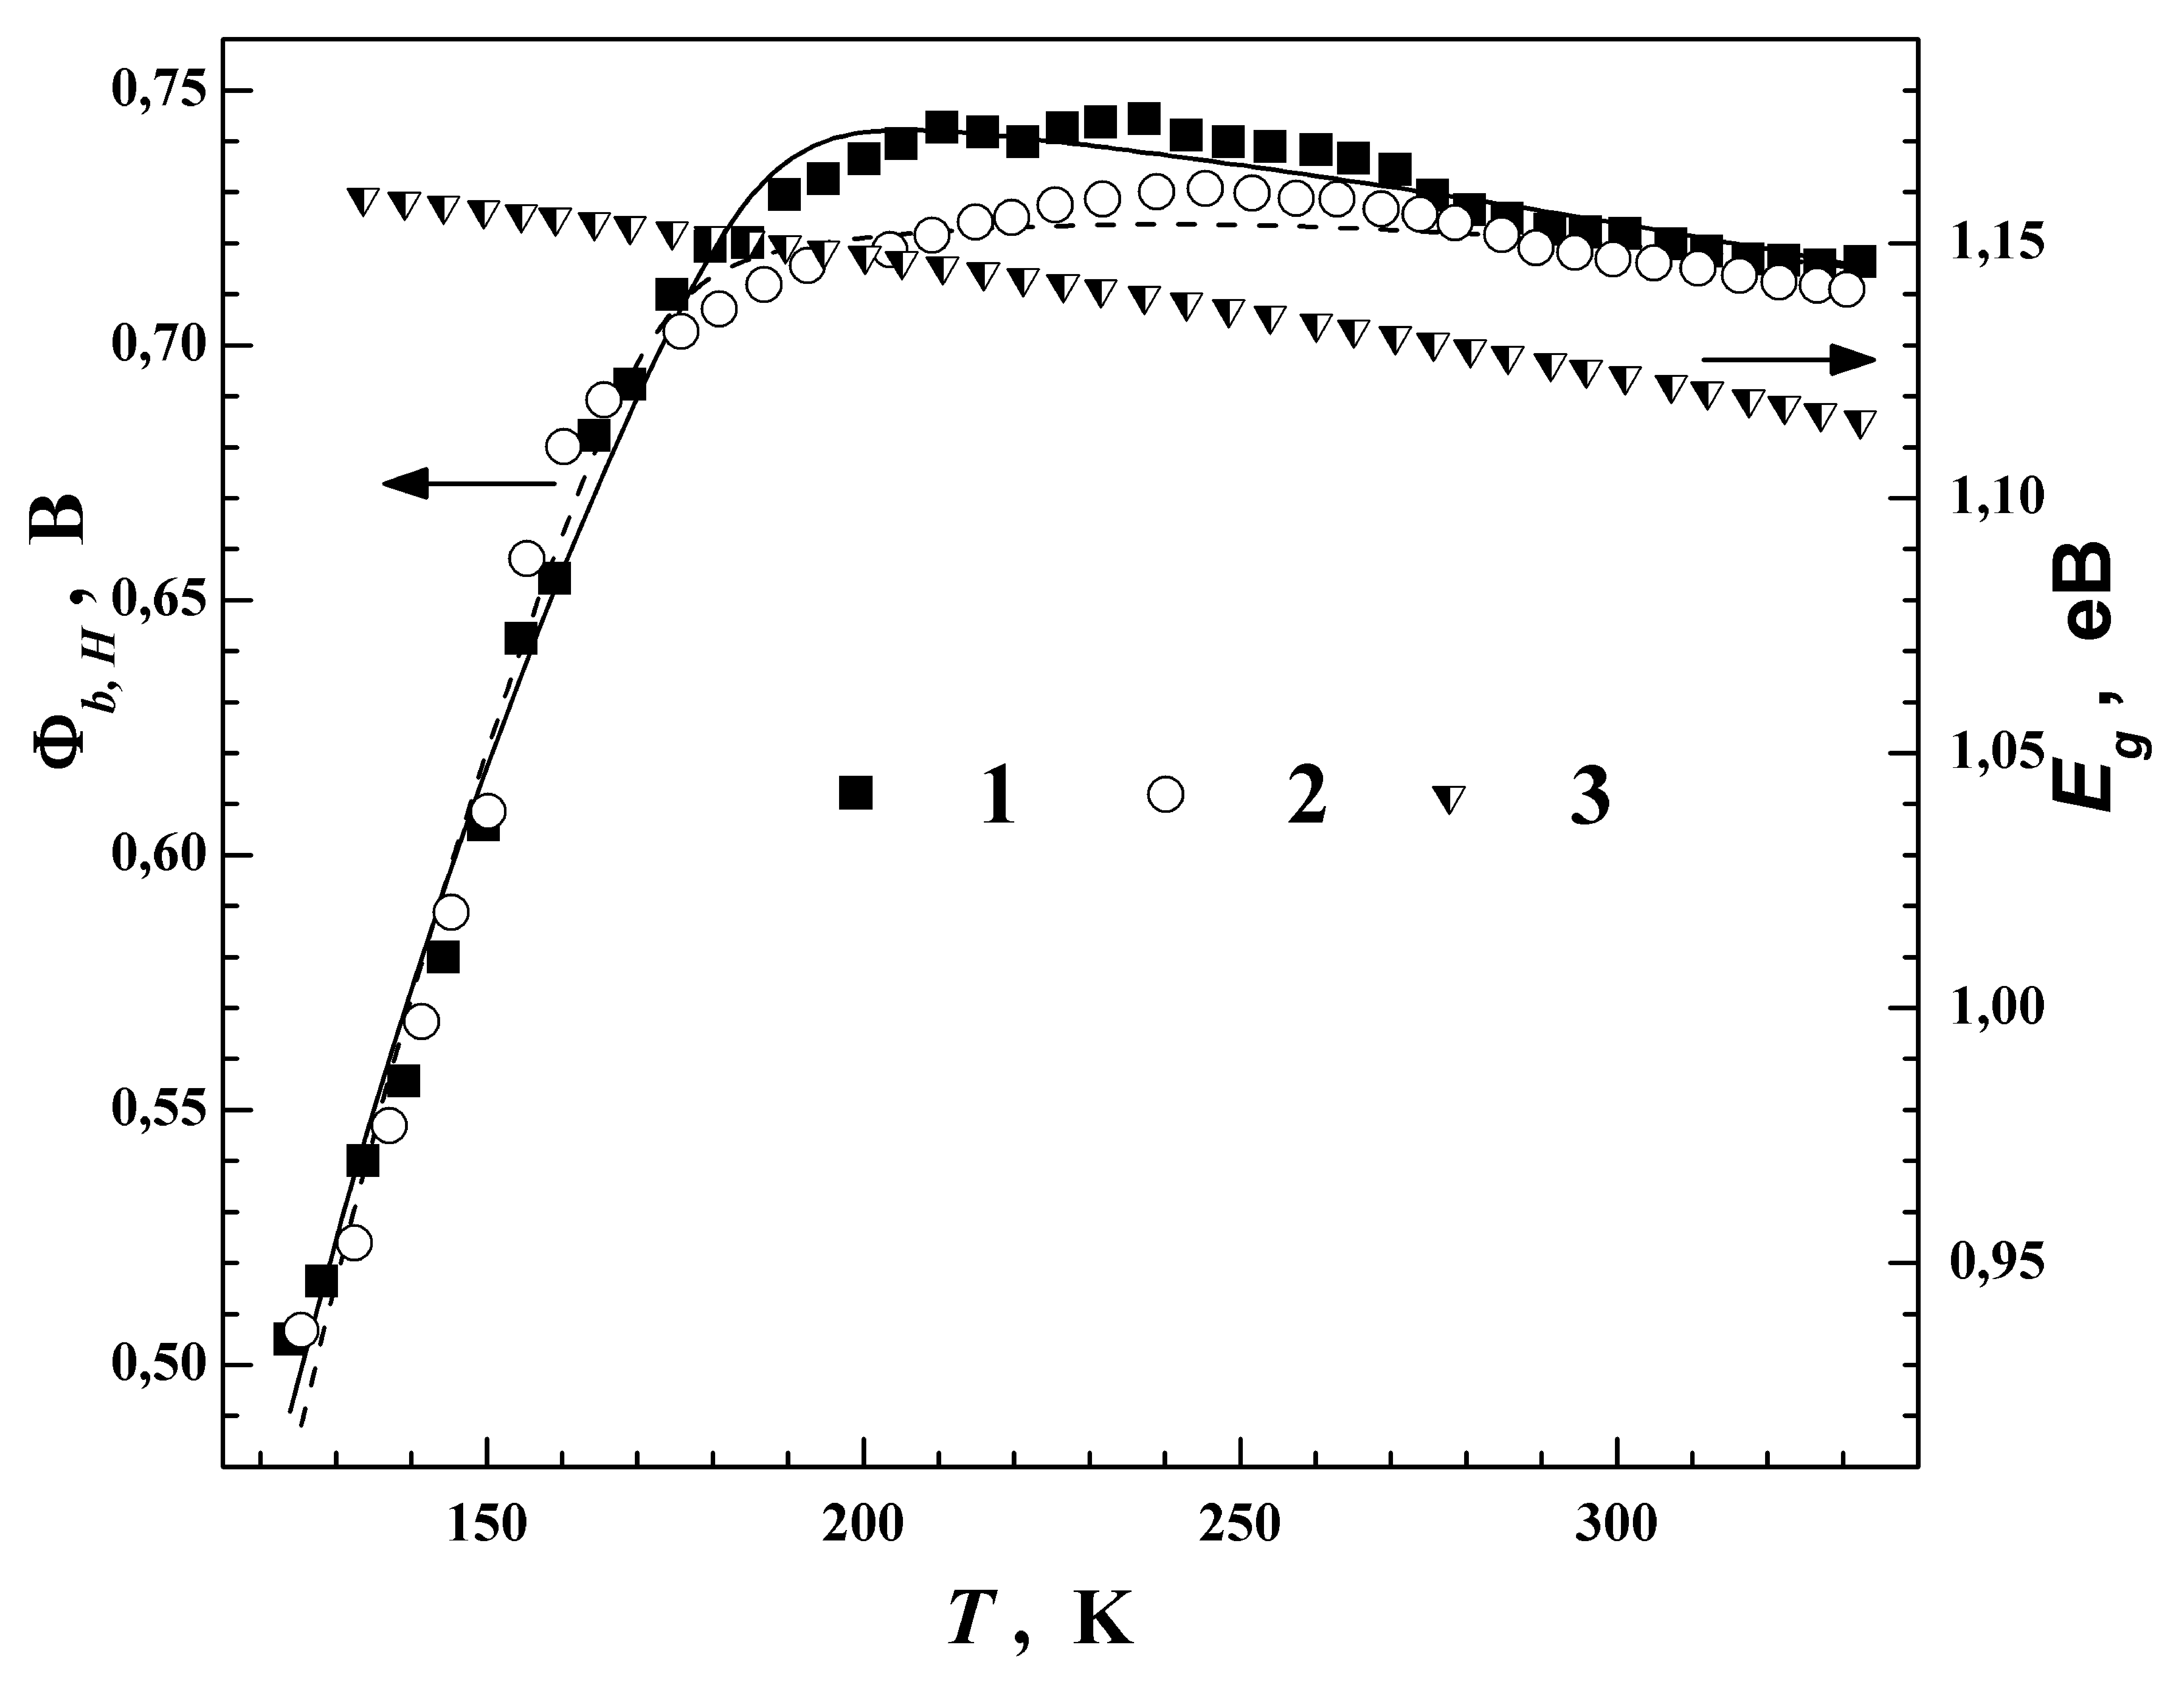
\includegraphics[width=0.8\textwidth]{figFbH_SDB}
\caption{\label{figFbH_SDB}
Температурні залежності ширина забороненої зони кремнію (3, права вісь)
та ВБШ при нульовому зміщенні структур SSDB в умовах U8SDB (2) та без нього (1).
Точки --- експеримент,
лінії --- апроксимація за формулою~(\ref{eqDG}).
$W_\mathtt{US}$,  Вт/см$^2$: 0 (1, суцільна лінія), 0,17 (2, штрихована лінія).
}%
\end{figure}


\begin{figure}
\center
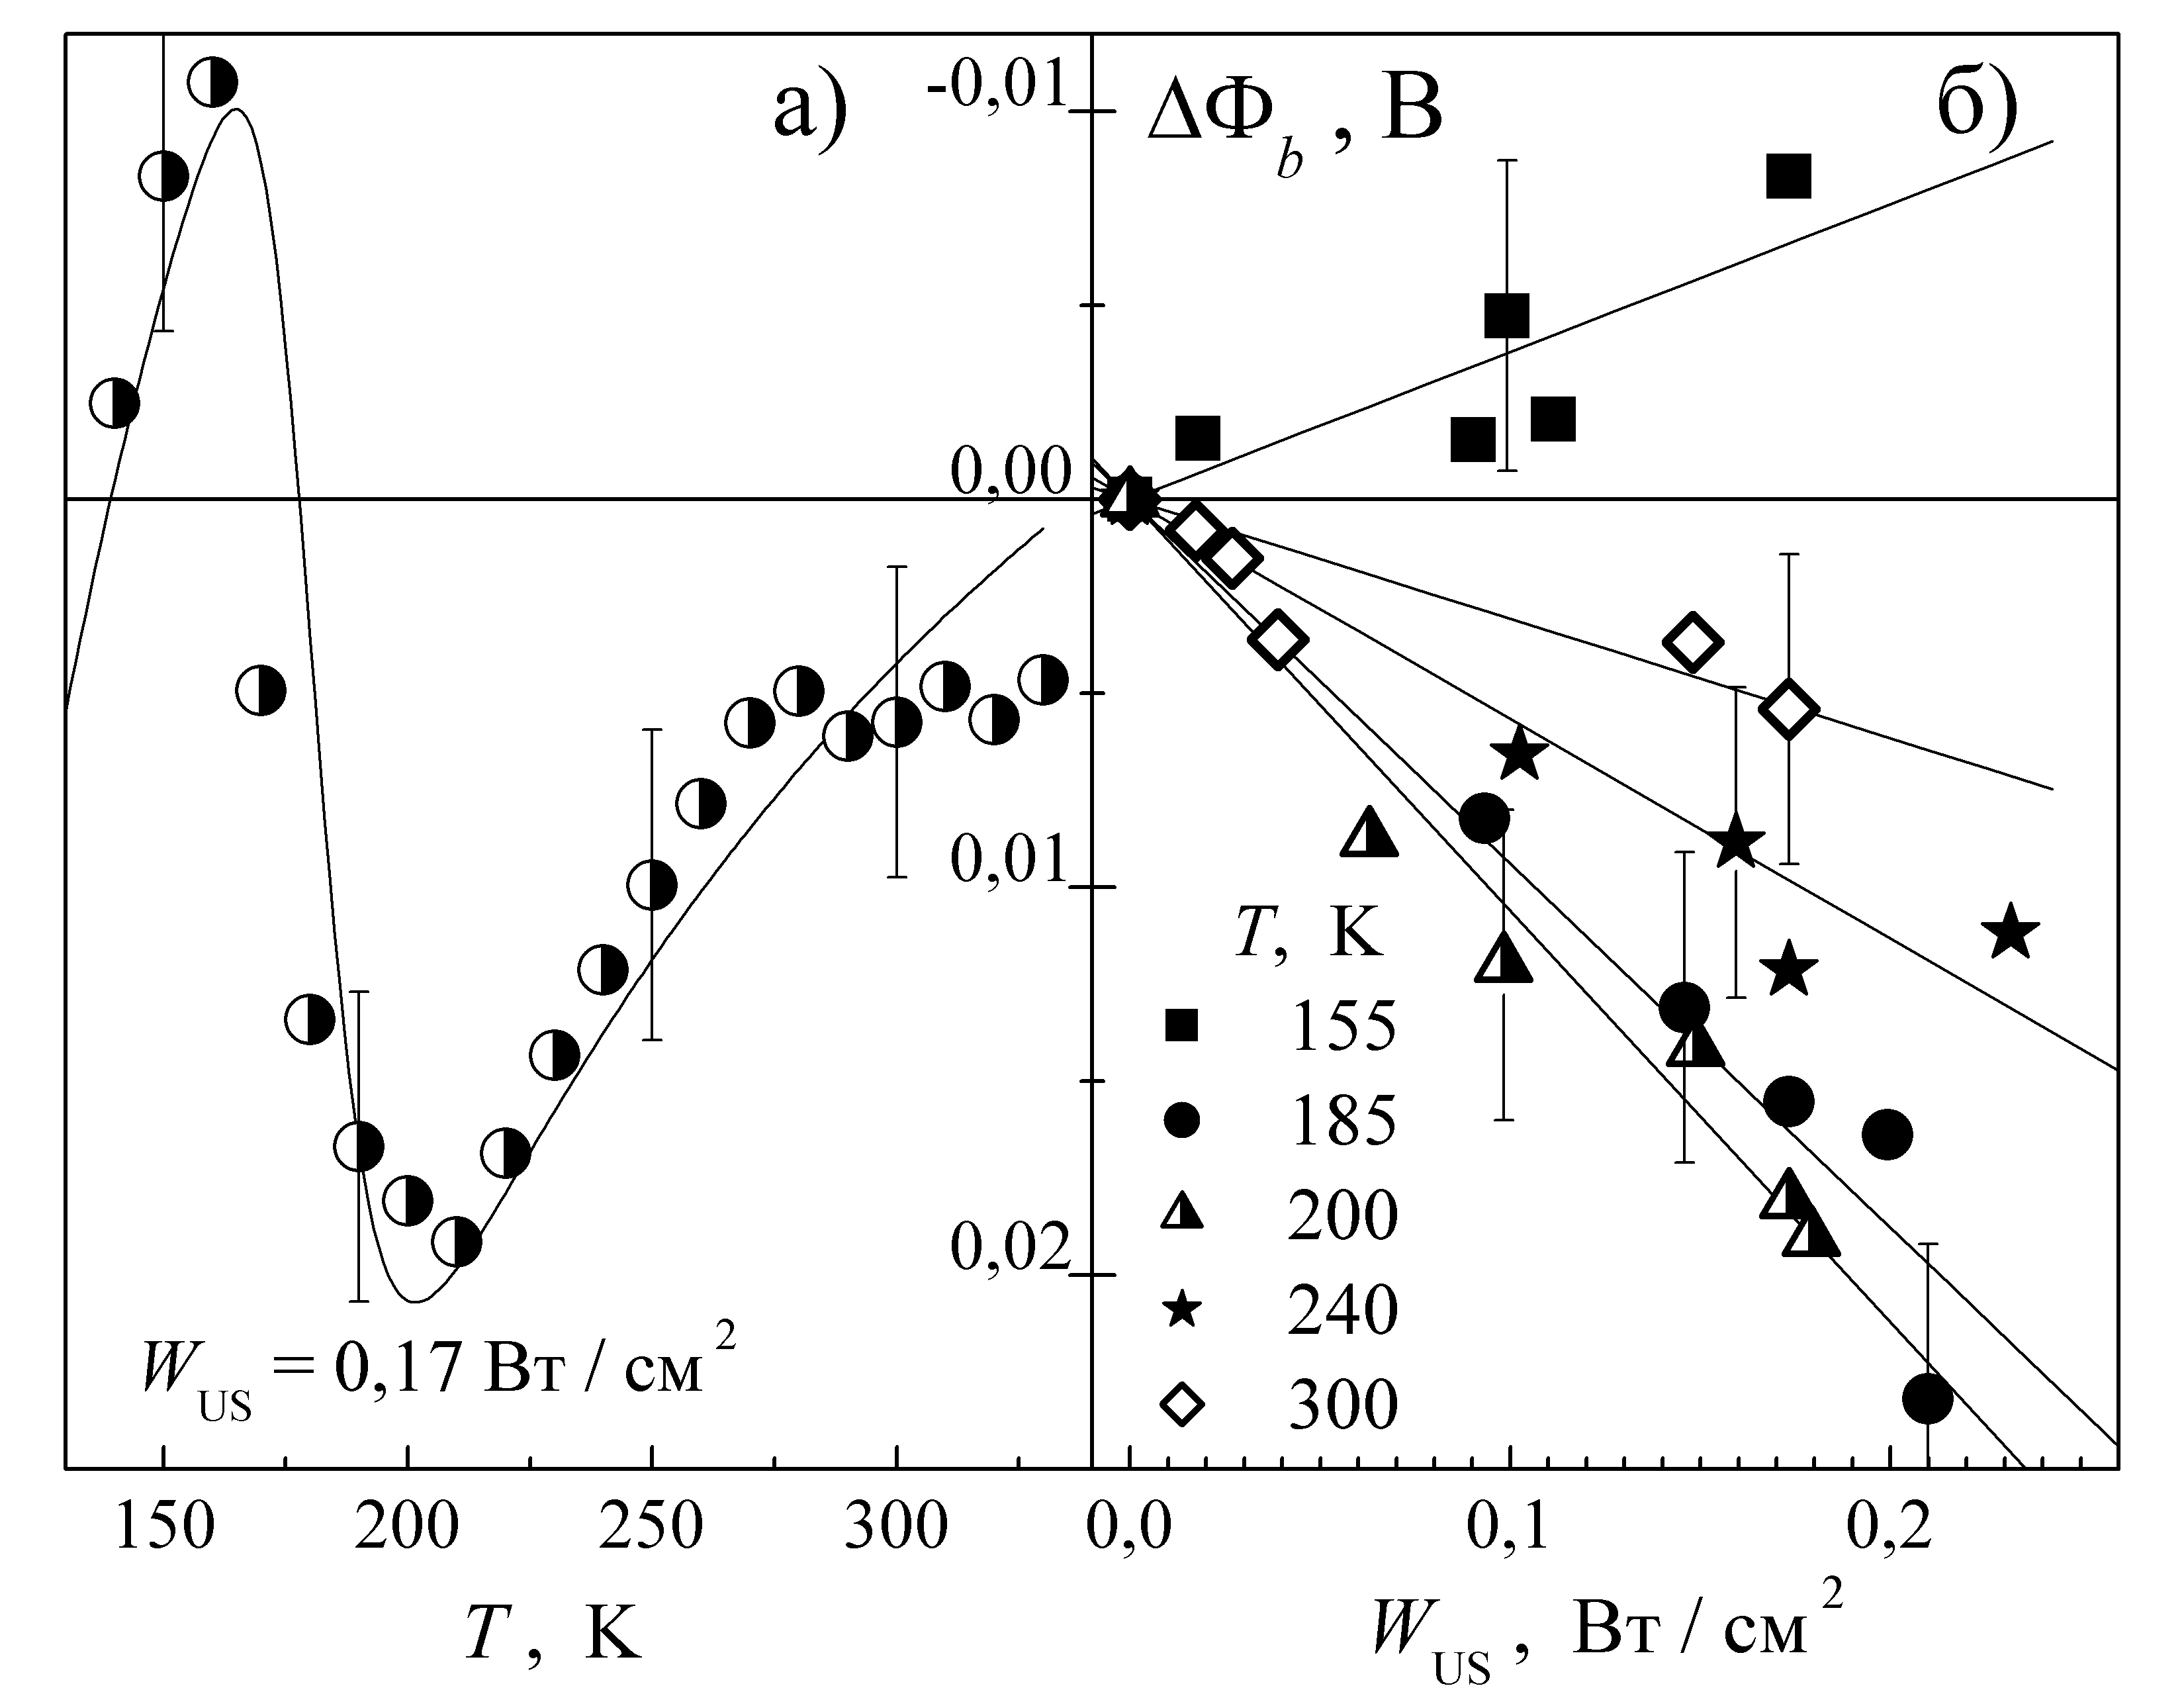
\includegraphics[width=0.8\textwidth]{figDelFbH}
\caption{\label{figDelFbH}
Залежності АІ змін висоти бар'єру ВТКС від температури (а) та інтенсивності введеного УЗ (б).
Точки ---експеримент,
лінія на рисунку (а) --- різниця між апроксимуючими кривими на Рис.~\ref{figFbH_SDB},
на рисунку (б) --- лінійна апроксимація.
U8SDB.
$T$, K: 155 (1), 185 (2), 200 (3), 240 (4), 300 (5).
}%
\end{figure}

Наведені результати показують, що
\begin{enumerate}[label=\asbuk*),leftmargin=0em,itemindent=1.5em]
\item АІ зміна висоти бар'єру є немотонною функцією температури, причому при $T<170$~K УЗН викликає зростання $\Phi_b$,
а при більших значеннях $T$ --- зменшення;
\item максимальне зменшення ВБШ спостерігається при $\sim210$~K і досягає 22~mV;
з підвищенням температури ефективність УЗ впливу УЗ зменшується;
\item величина зміни ВБШ збільшується при зростанні інтенсивності УЗ; відповідні залежності при кожній з температур
близькі до лінійних.
\end{enumerate}
Очевидно, що для розуміння можливих причин впливу УЗ необхідно проаналізувати механізм перенесення заряду
у досліджених структурах.

Як вже неодноразово згадувалося раніше, для однорідного контакту Шотки висота бар'єру при зміні температури має змінюватися подібно
до ширини забороненої зони \cite{Rhoderick1988,Aboelfotoh,Zhua}.
І тому традиційно, поряд з температурною залежністю ВБШ на Рис.~\ref{figFbH_SDB} також наведено графік $E_g(T)$,
розрахований з використанням виразу (\ref{eqEg}).
Виявлено, що загалом ці залежності схожі при $T>200$~K.
Крім того, на Рис.~\ref{figRich_SDB} представлено залежності Річардсона, розраховані згідно з
виразом (\ref{eqRich}) для ВТКС в діапазоні температур $200\div330$~K.
Як і очікується для однорідного контакту, ці залежності близькі до лінійних,
проте отримані значення сталої Річардсона $1060$~A$\cdot$см$^{-2}\cdot$K$^{-2}$ та $65$~A$\cdot$см$^{-2}\cdot$K$^{-2}$
для структур без акустичного навантаження та в умовах УЗН, відповідно, суттєво відрізняються
від табличного ($112$~A$\cdot$см$^{-2}\cdot$K$^{-2}$ для $n$--Si).


\begin{figure}
\center
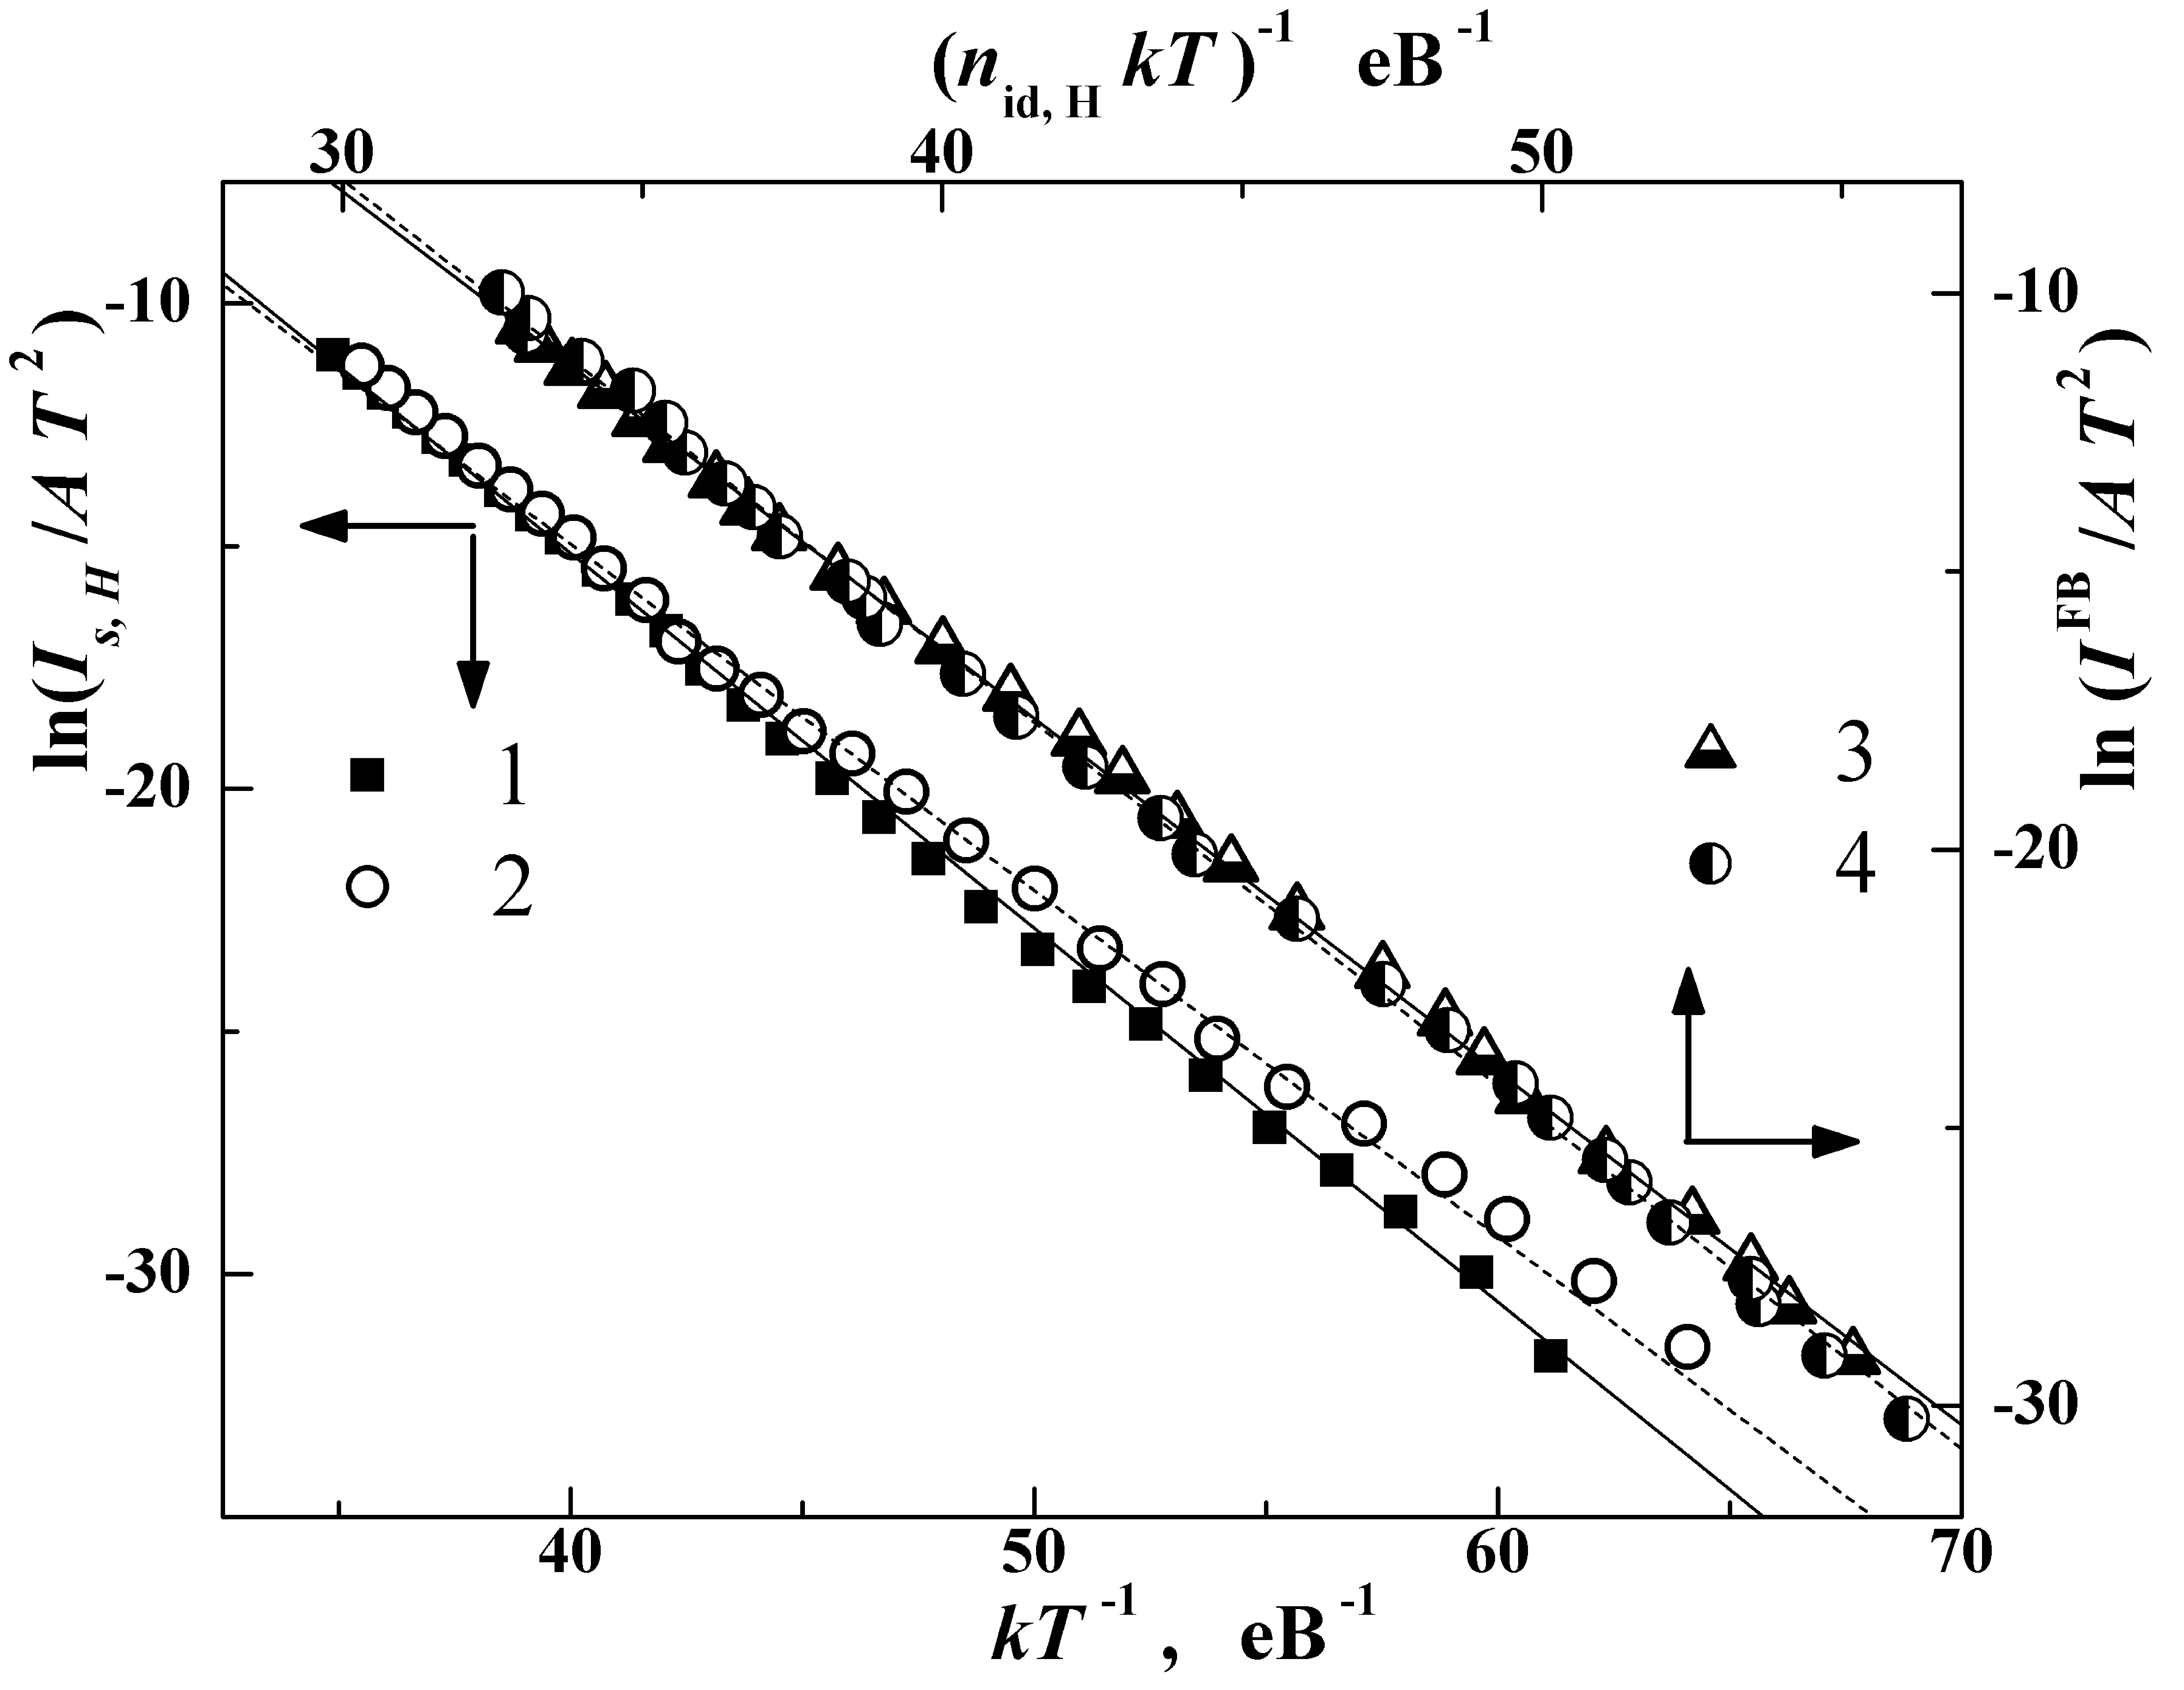
\includegraphics[width=0.7\textwidth]{figRich_SDB}
\caption{\label{figRich_SDB}
Звичайні (відповідно до формули(\ref{eqRich}), криві 1 та 2)
та модифіковані (відповідно до формули(\ref{eqRichFB}), 3 та 4)
залежності Річардсона для структур SSDB за умов U8SDB (2, 4) та без нього (1, 3) побудовані в інтервалі
температур $200\div330$~K.
Точки --- експеримент, лінії --- лінійна апроксимація (суцільні --- без УЗН).
$W_\mathtt{US}$,  Вт/см$^2$: 0 (1, 3), 0,17 (2, 4).
}%
\end{figure}

Подібну поведінку залежності Річардсона зазвичай пов'язують з польовою та температурною залежностями ВБШ та фактору неідеальності,
які виникають внаслідок неоднорідності контакту МН \cite{Sarpatwari,Aldemir}.
З іншого боку, за умов плоских зон вплив латеральних неоднорідностей несуттєвий \cite{Aldemir,Unewisse,Korkut}.
Використовуючи визначені традиційним способом з експериментальних ВАХ значення $n_\mathrm{id}$, $\Phi_b$ та $I_s$,
можна розрахувати ВБШ $\Phi_{b}^\mathrm{FB}$ (формула~(\ref{eqFbfb})) та струм насичення $I^\mathrm{FB}$ в наближені плоских зон \cite{Aldemir,Unewisse,Korkut}:
\begin{equation}\label{eqIfb}
I^\mathrm{FB}=I_s\exp\left[\frac{qV_n(n_\mathrm{id}-1)}{n_\mathrm{id}kT}\right]\,.
\end{equation}
Більше того, температурна залежність $\Phi_{b}^\mathrm{FB}$ може бути записана наступним чином
\begin{equation}
\label{eqFFT}
\Phi_{b}^\mathrm{FB}(T)=\Phi_{b}^\mathrm{FB}(0)+\alpha_\mathrm{\,FB} T \,,
\end{equation}
де
$\Phi_{b}^\mathrm{FB}(0)$ --- ВБШ за умови плоских зон, екстрапольована до $T = 0$~K,
$\alpha_\mathrm{\,FB}$ --- температурний коефіцієнт.
Температурна залежність $\Phi_{b}^\mathrm{FB}$ для ВТКС показана на Рис.~\ref{figFf_SDB}.
Апроксимація даних на Рис.~\ref{figFf_SDB} відповідно до формули~(\ref{eqFFT}) дозволила
визначити величини  $\Phi_{b}^\mathrm{FB}(0)$ та $\alpha_\mathrm{\,FB}$,
наведені в Таблиці~\ref{tabSDBPar}.


\begin{figure}
\center
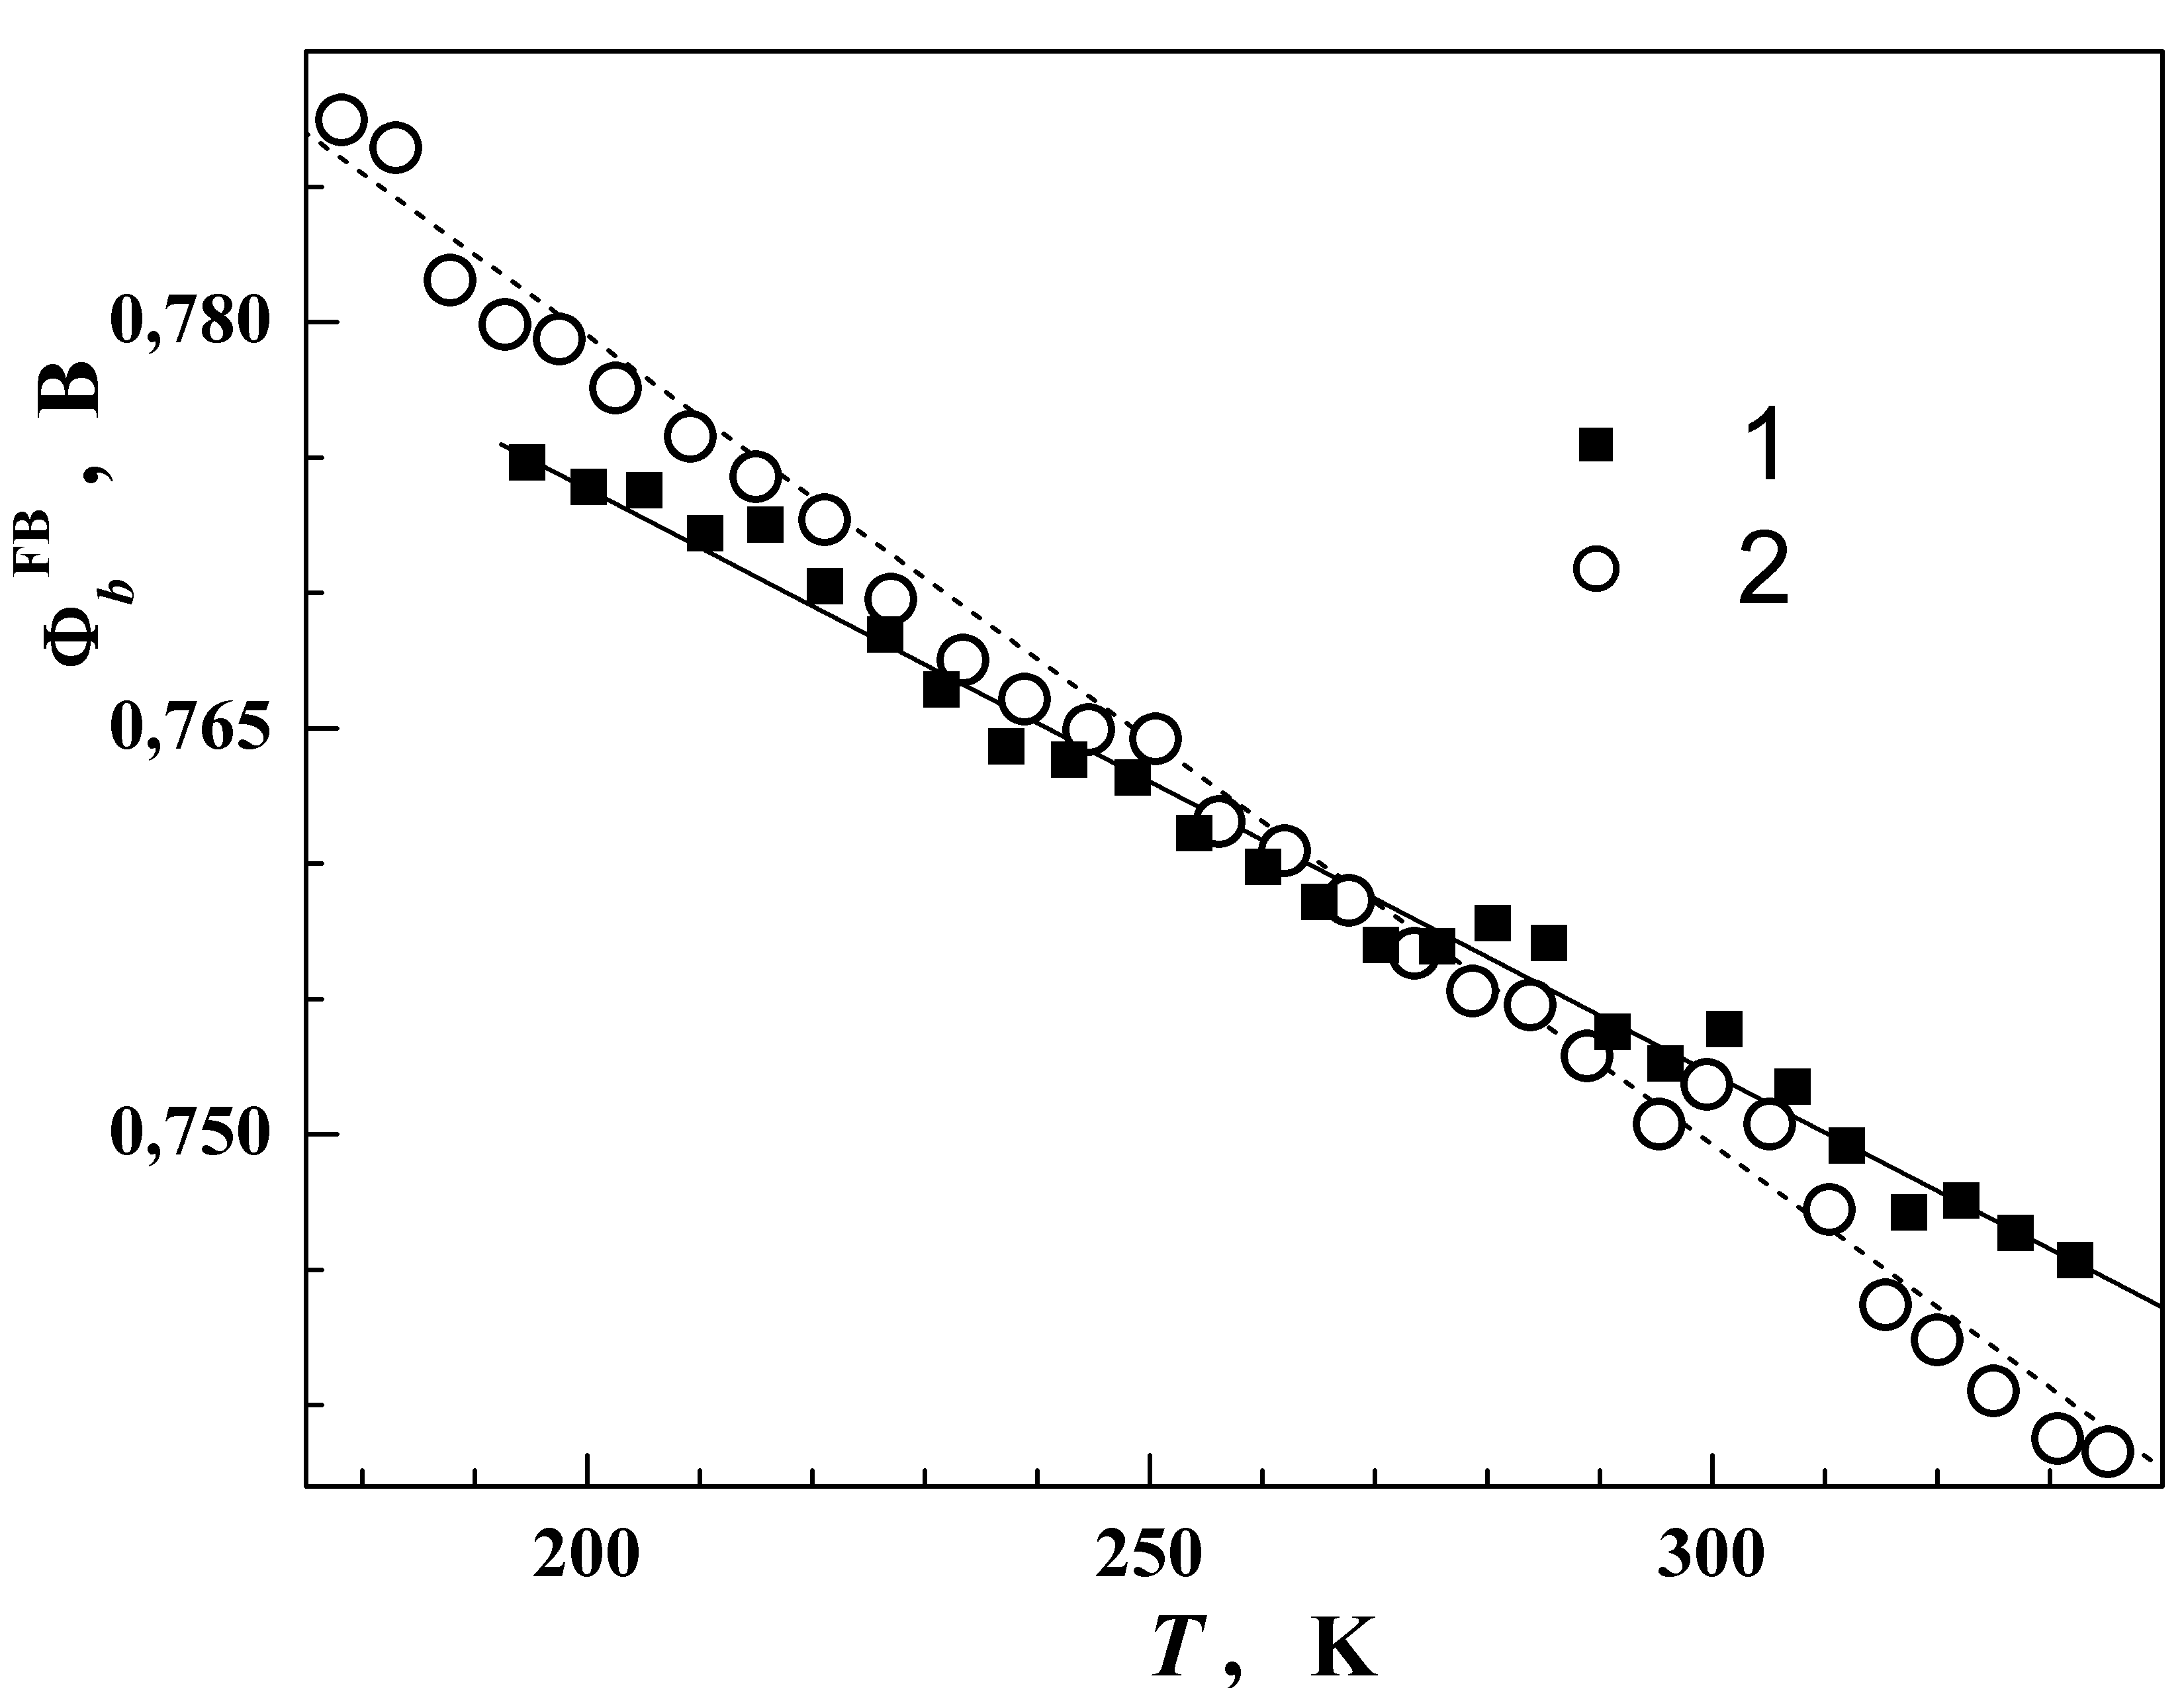
\includegraphics[width=0.7\textwidth]{figFf_SDB}
\caption{\label{figFf_SDB}
Температурна залежність висоти бар'єру Шотки в наближенні плоских зон
структур SSDB за умов U8SDB (2) та без нього (1) побудовані в інтервалі
температур $200\div330$~K.
Точки --- експеримент, лінії --- лінійна апроксимація (суцільна --- без УЗН).
$W_\mathtt{US}$,  Вт/см$^2$: 0 (1), 0,17 (2).
}%
\end{figure}


\begin{table}
\caption{Параметри, визначені для структур Mo$/n-n^+$--Si з прямих гілок ВАХ}
\label{tabSDBPar}
\centering
\begin{tabular}{|l|c|c|}
\hline
$W_\mathtt{US}$,  Вт/см$^2$ &0&0,17\\\hline
\hline
$\alpha_\mathrm{\,FB}$, мВ/K &$-0,22\pm0,02$&$-0,30\pm0,02$\\\hline
$\Phi_{b}^\mathrm{FB}(0)$, мВ \textsuperscript{ a)} &$817\pm4$ & $839\pm5$\\\hline
$\Phi_{b}^\mathrm{FB}(0)$, мВ \textsuperscript{ б)} &$821\pm4$ & $845\pm5$\\\hline
$A^*$, A$\cdot$см$^{-2}\cdot$K$^{-2}$ &$116\pm5$ & $111\pm5$\\\hline
$\varrho_1$ &$0,9995$ & $0,998$\\\hline
$\varrho_2$ &$0,5\cdot10^{-3}$ & $2\cdot10^{-3}$\\\hline
$\sigma_{\Phi0,1}$, мВ&$18\pm2$ & $48\pm4$\\\hline
$\sigma_{\Phi0,2}$, мВ&$118\pm5$ & $127\pm5$\\\hline
$\Phi_{b,1}^0(0)$, мВ&$775\pm8$ & $809\pm8$\\\hline
$\Phi_{b,2}^0(0)$, мВ&$1070\pm50$ & $1170\pm50$\\\hline
$T_{0,H}$, K&$14\pm1$&$18\pm1$\\\hline
$T_{0,L}$, K&$130\pm5$&$143\pm5$\\\hline
$\gamma_p$, $10^{-5}$ м$^{2/3}\cdot$В$^{1/3}$&$2,7\pm0,1$&$2,5\pm0,1$\\\hline
$C_p$, $10^{5}$ м$^{-2}$&$2,2\pm0,4$&$21\pm3$\\ \hline
\multicolumn{3}{l}{\textsuperscript{ a)} \emph{за формулою~(\ref{eqFFT}), Рис.~\ref{figFf_SDB} }}  \\
\multicolumn{3}{l}{\textsuperscript{ б)} \emph{за формулою~(\ref{eqRichFB}), Рис.~\ref{figRich_SDB} }} \\
\end{tabular}
\end{table}

Згідно з даними класичного підручника \cite{Rhoderick1988},
ВБШ в наближенні плоских зон може бути записаний наступним чином
\begin{equation}
\label{eqFbfRoder}
    q\Phi_{b}^\mathrm{FB}=\Theta(\phi_m-\chi_s)+(1-\Theta)(E_g-\varphi_0)
\end{equation}
де $\Theta=[1+(qD_{ss}\delta)/(\varepsilon_0\varepsilon_i)]^{-1}$,
$\phi_m$ --- робота виходу з металу,
$\chi_s$ --- електронна спорідненість напівпровідника (4.05~еВ для Si),
$\delta_i$ та $\varepsilon_i$ --- товщина та діелектрична проникність оксидного шару між металом та напівпровідником.
Вираз~(\ref{eqFbfRoder}) не враховує зниження бар'єру внаслідок дії сил зображень.
Для молібдену робота виходу залежить від кристалографічної площини та умов виготовлення контакту
і знаходиться в межах від 4,53 до 4,95~еВ для структури Mo/Si \cite{MoWF2002}.
Таким чином, величина $\Phi_{b}^\mathrm{FB}$ має прямувати до границі Шотки--Мота
$q\Phi_{b}^\mathrm{FB,SM}=\phi_m-\chi_s=(0,48\div0,90)$~еВ при $D_{ss}\rightarrow0$
та до границі Бардіна $q\Phi_{b}^\mathrm{FB,B}=E_g-\phi_0$ при $D_s\rightarrow\infty$.
Отримана для досліджених структур величина знаходиться в межах цього теоретично можливого інтервалу.

В наближенні плоских зон зазвичай розглядається модифікована залежність Річардсона:
\begin{equation}
\label{eqRichFB}
\ln\left(\frac{I^\mathrm{FB}}{A\,T^2}\right)=\ln A^*_{mod}-\frac{q\Phi_{b}^\mathrm{FB}(0)}{n_\mathrm{id}kT}\,,
\end{equation}
де модифікована стала Річардсона $A^*_{mod}$  пов'язана зі звичайною $A^*$  співвідношенням
\begin{equation}
\label{eqAmod}
A^*=A^*_{mod}\exp\left(\frac{q\alpha_\mathrm{\,FB}}{k}\right).
\end{equation}
На Рис.~\ref{figRich_SDB} (криві 3 та 4) показані модифіковані залежності для ВТКС.
Значення $\Phi_{b}^\mathrm{FB}(0)$ та $A^*_{mod}$ були визначені з цього графіку шляхом апроксимації відповідно до формули~(\ref{eqRichFB})
для навантаженого та ненавантаженого зразка.
Після цього, з використанням виразу~(\ref{eqAmod}), були обчислені величини $A^*$ для цих випадків.
Отримані результати представлені в Таблиці~\ref{tabSDBPar}.
Наголосимо, що
а)~значення $A^*$ дуже близькі до відомих для даного матеріалу і не залежать від УЗН;
б)~ВБШ в наближенні плоских зон збільшується при дії УЗ;
на нашу думку це збільшення пов'язане з АІ зменшенням $\varphi_0$ (модифікацією заряду інтерфейсних станів).

Відмінність між даними, отриманими з модифікованої та звичайної залежностей Річардсона,
а також характер зміни $\Phi_{b,H}$ у всьому температурному діапазоні $130\div330$~K (Рис.~\ref{figFbH_SDB})
свідчать на користь необхідності застосування моделі неоднорідного бар'єру Шотки.
Як вже згадувалось у попередньому розділі,
неоднорідну поверхню розділу між металом та напівпровідником можна описати в наближенні загалом однорідної області,
яка містить хаотичним чином розміщені ділянки (патчі) зі зменшеною ВБШ \cite{Tung:PhysRev,Tung:MSE}.
Окремий патч характеризується величиною $\gamma_p$ (див. вираз ~(\ref{eqGammaP})),
його зміни на масиві ділянок неоднорідності описуються розподілом Гауса.
При цьому висота бар'єру, визначена з ВАХ (в нашому випадку --- $\Phi_{b,H}$) пов'язана з ВБШ в однорідній області співвідношенням (\ref{eqFb0T}).

Проте експериментально виявлені залежності ВБШ від оберненої температури нерідко не мають вигляд прямої лінії \cite{KumarJAP2012,Tascioglu2010,Jiang:DG,Yildirima:DG,Jiang:DGJap},
як це очікується з виразу (\ref{eqFb0T}).
У зв'язку з цим було запропоновано описувати неоднорідність контакту Шотки за допомогою концепції подвійного розподілу Гауса \cite{Jiang:DG,Yildirima:DG,Jiang:DGJap}.
А саме, в цьому наближенні ВБШ може бути записана наступним чином:
\begin{equation}
\label{eqDG}
  \Phi_b=-\frac{kT}{q}\ln\left[\varrho_1\exp\left(-\frac{q\Phi_{b,1}^0}{kT}+
  \frac{q^2\sigma^2_{\Phi0,1}}{2k^2T^2}\right)
   +
  \varrho_2\exp\left(-\frac{q\Phi_{b,2}^{0}}{kT}+
  \frac{q^2\sigma^2_{\Phi0,2}}{2k^2T^2}\right)\right],
\end{equation}
де
$\varrho_1$, $\varrho_2=1-\varrho_1$, $\sigma_{\Phi0,1}$, $\sigma_{\Phi0,2}$, $\Phi_{b,1}^0$ та $\Phi_{b,2}^0$ ---
вагові коефіцієнти, стандартні відхилення та середні значення двох розподілів Гауса, відповідно.

Для структур SSDB залежність $\Phi_{b,H}$ від $1/T$ також не є прямою для всього температурного інтервалу $130\div330$~K.
Була проведена апроксимація експериментальних даних відповідно до вираз~(\ref{eqDG}).
При цьому вважалося, що температурна залежність $\Phi_{b,i}^0$ описується формулою~(\ref{eqFbT}), а величини
$\varrho_1$, $\sigma_{\Phi0,1}$, $\sigma_{\Phi0,2}$ та середні значення ВБШ при нульовій температурі $\Phi_{b,1}^0(0)$ та $\Phi_{b,2}^0(0)$
розглядалися як невідомі параметри.
Результати апроксимації представлені лініями на Рис.~\ref{figFbH_SDB} та даними в Таблиці~\ref{tabSDBPar}.
Різниця між апроксимуючими залежність $\Phi_{b,H}(T)$ кривими для структур за умов УЗН та без нього
показана лінією на Рис.~\ref{figDelFbH},a.
Видно, що спостерігається досить непогане узгодження між експериментальними даними та апроксимуючими кривими.

Відповідно до роботи \cite{Jiang:DGJap},
розподіл Гауса з меншим внеском (меншою величиною $\varrho$) пов'язаний з патчами, причиною появи яких є
неповна та неоднорідна дифузія атомів металу.
Отже, в нашому випадку з цими дефектами можуть бути пов'язані $\Phi_{b,2}^0$ та $\sigma_{\Phi0,2}$.
Величина $\Phi_{b,2}^0$ свідчить про те, що таким патчам властиві високе значення густини інтерфейсних станів та низьке значення рівня нейтральності --- див. формулу~(\ref{eqFbfRoder}).
Водночас $\Phi_{b,1}^0$ пов'язана саме з однорідною частиною контакту,
а $\sigma_{\Phi0,1}$ описує патчі іншої природи, які, згідно з \cite{Gammon2013}, можуть бути пов'язані з шорсткістю поверхні,
нерівномірним профілем розподілу легуючої домішки, кристалічними дефекти тощо.
В роботі \cite{Rhoderick1988} показано, що ВБШ має бути нижчою ніж величина, яка отримується в наближенні плоских зон,
причому різниця пропорційна максимальному значенню напруженості електричного поля.
Для визначених величин виконується співвідношення $\Phi_{b}^\mathrm{FB}>\Phi_{b,1}^0$, що  збігається з передбаченим співвідношенням.

Як видно з Таблиці~\ref{tabSDBPar}, як середнє значення ВБШ, так і стандартне відхилення ВБШ збільшується під дією УЗ.
Оборотне збільшення ВБШ, на нашу думку, пов'язане з перезарядкою чи конфігураційною перебудовою інтерфейсних дефектів в полі напруг
АХ, що і є причиною зсуву рівня нейтральності.
Подібні АІ ефекти спостерігалися і раніше, зокрема описані у попередніх розділах.
Уширення розподілу $\gamma_p$ (збільшення $\sigma_{\Phi0}$) з неоднаковим впливом УЗН на патчі з різними параметрами.

На Рис.~\ref{figfigNh_SDB} показано температурну залежність фактору неідеальності ВТКС.
Як видно з рисунку, в температурному інтервалі $180\div250$~K спостерігається АІ збільшення $n_\mathrm{id}$.
Ефективність впливу УЗН з підвищенням температури зменшується --- див. вставку на Рис.~\ref{figfigNh_SDB}.

\begin{figure}
\center
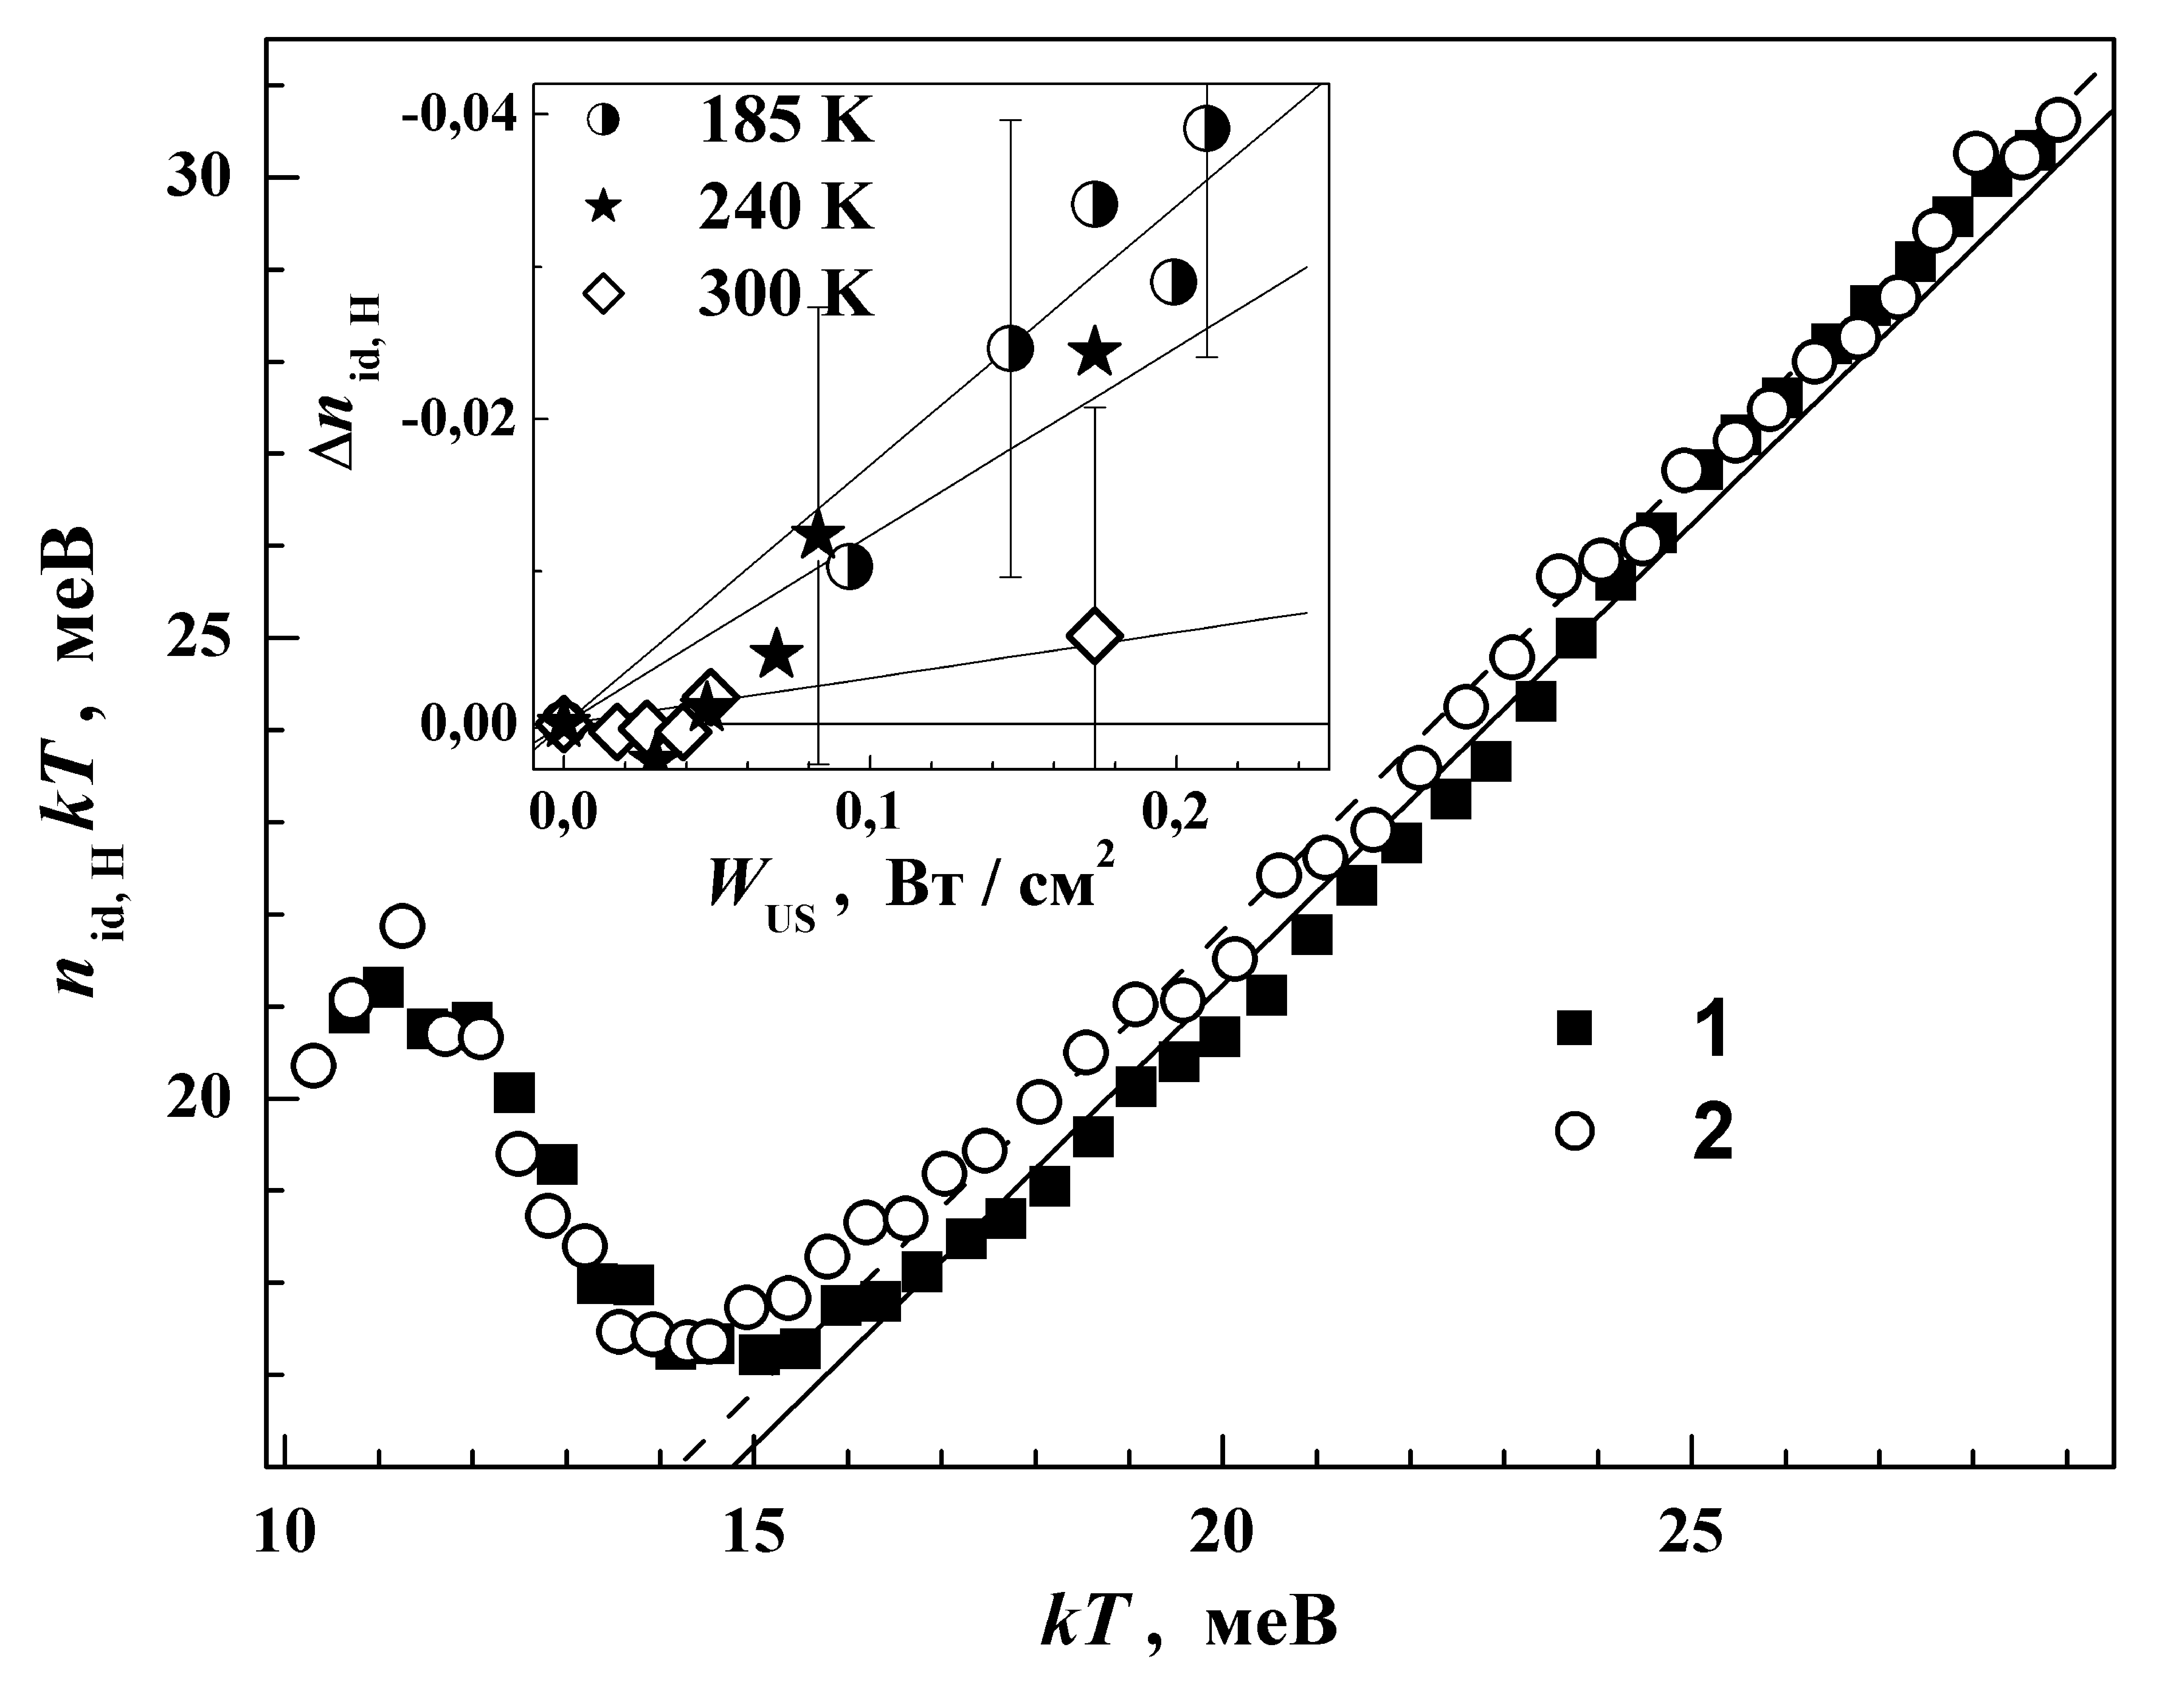
\includegraphics[width=0.7\textwidth]{figfigNh_SDB}
\caption{\label{figfigNh_SDB}
Залежність $n_\mathrm{id,H}kT$ від оберненої температури для структур SSDB за умов U8SDB (2) та без нього (1).
Точки --- експеримент, лінії --- апроксимація відповідно до формули~(\ref{eqN_T:TE}) в інтервалі
температур $200\div330$~K (суцільна --- без УЗН).
$W_\mathtt{US}$,  Вт/см$^2$: 0 (1), 0,17 (2).
На вставці залежності АІ змін фактору неідеальності від інтенсивності УЗ при різних температурах;
точки --- експеримент, лінії --- лінійна апроксимація.
}%
\end{figure}

Як вже згадувалося, температурна залежність фактору неідеальності нерідко описується за допомогою формули (\ref{eqN_T:TE}).
Саме вона і була використана для апроксимації експериментальних даних в діапазоні $200\div330$~K.
Результати апроксимації представлені на рисунку (лінії) та в Таблиці~\ref{tabSDBPar} (значення $T_{0,H}$).
У випадку неоднорідного контакту, $T_0$ пов'язано з розподілом параметрів патчів
за допомогою співвідношення (\ref{eqN_T0}) і тому виявлена тенденція
збільшення $T_{0,H}$ за умов УЗН якісно співпадає з АІ збільшенням $\sigma_{\Phi0}$.





\subsection{Характеристики низько--температурної компоненти струму}

Формула~(\ref{eqFb:TE}) була також використана для обчислення висоти бар'єру НТКС $\Phi_{b,L}$, температурна залежність
якої представлена на Рис.~\ref{figFbL_SDB},а.
На другій частині цього рисунка наведена амплітудна залежність змін ВБШ $\Delta \Phi_{b,L}$ під дією УЗ.
Видно, що $\Phi_{b,L}$ збільшується при малих інтенсивностях пружних коливань та низьких температурах,
тоді як при високих значеннях $T$ або при збільшенні $W_\mathtt{US}$ спостерігаються протилежні зміни ВБШ.
Подібна немонотонна залежність свідчить про наявність двох конкуруючих механізмів ультразвукового впливу на $\Phi_{b,L}$.


\begin{figure}
\center
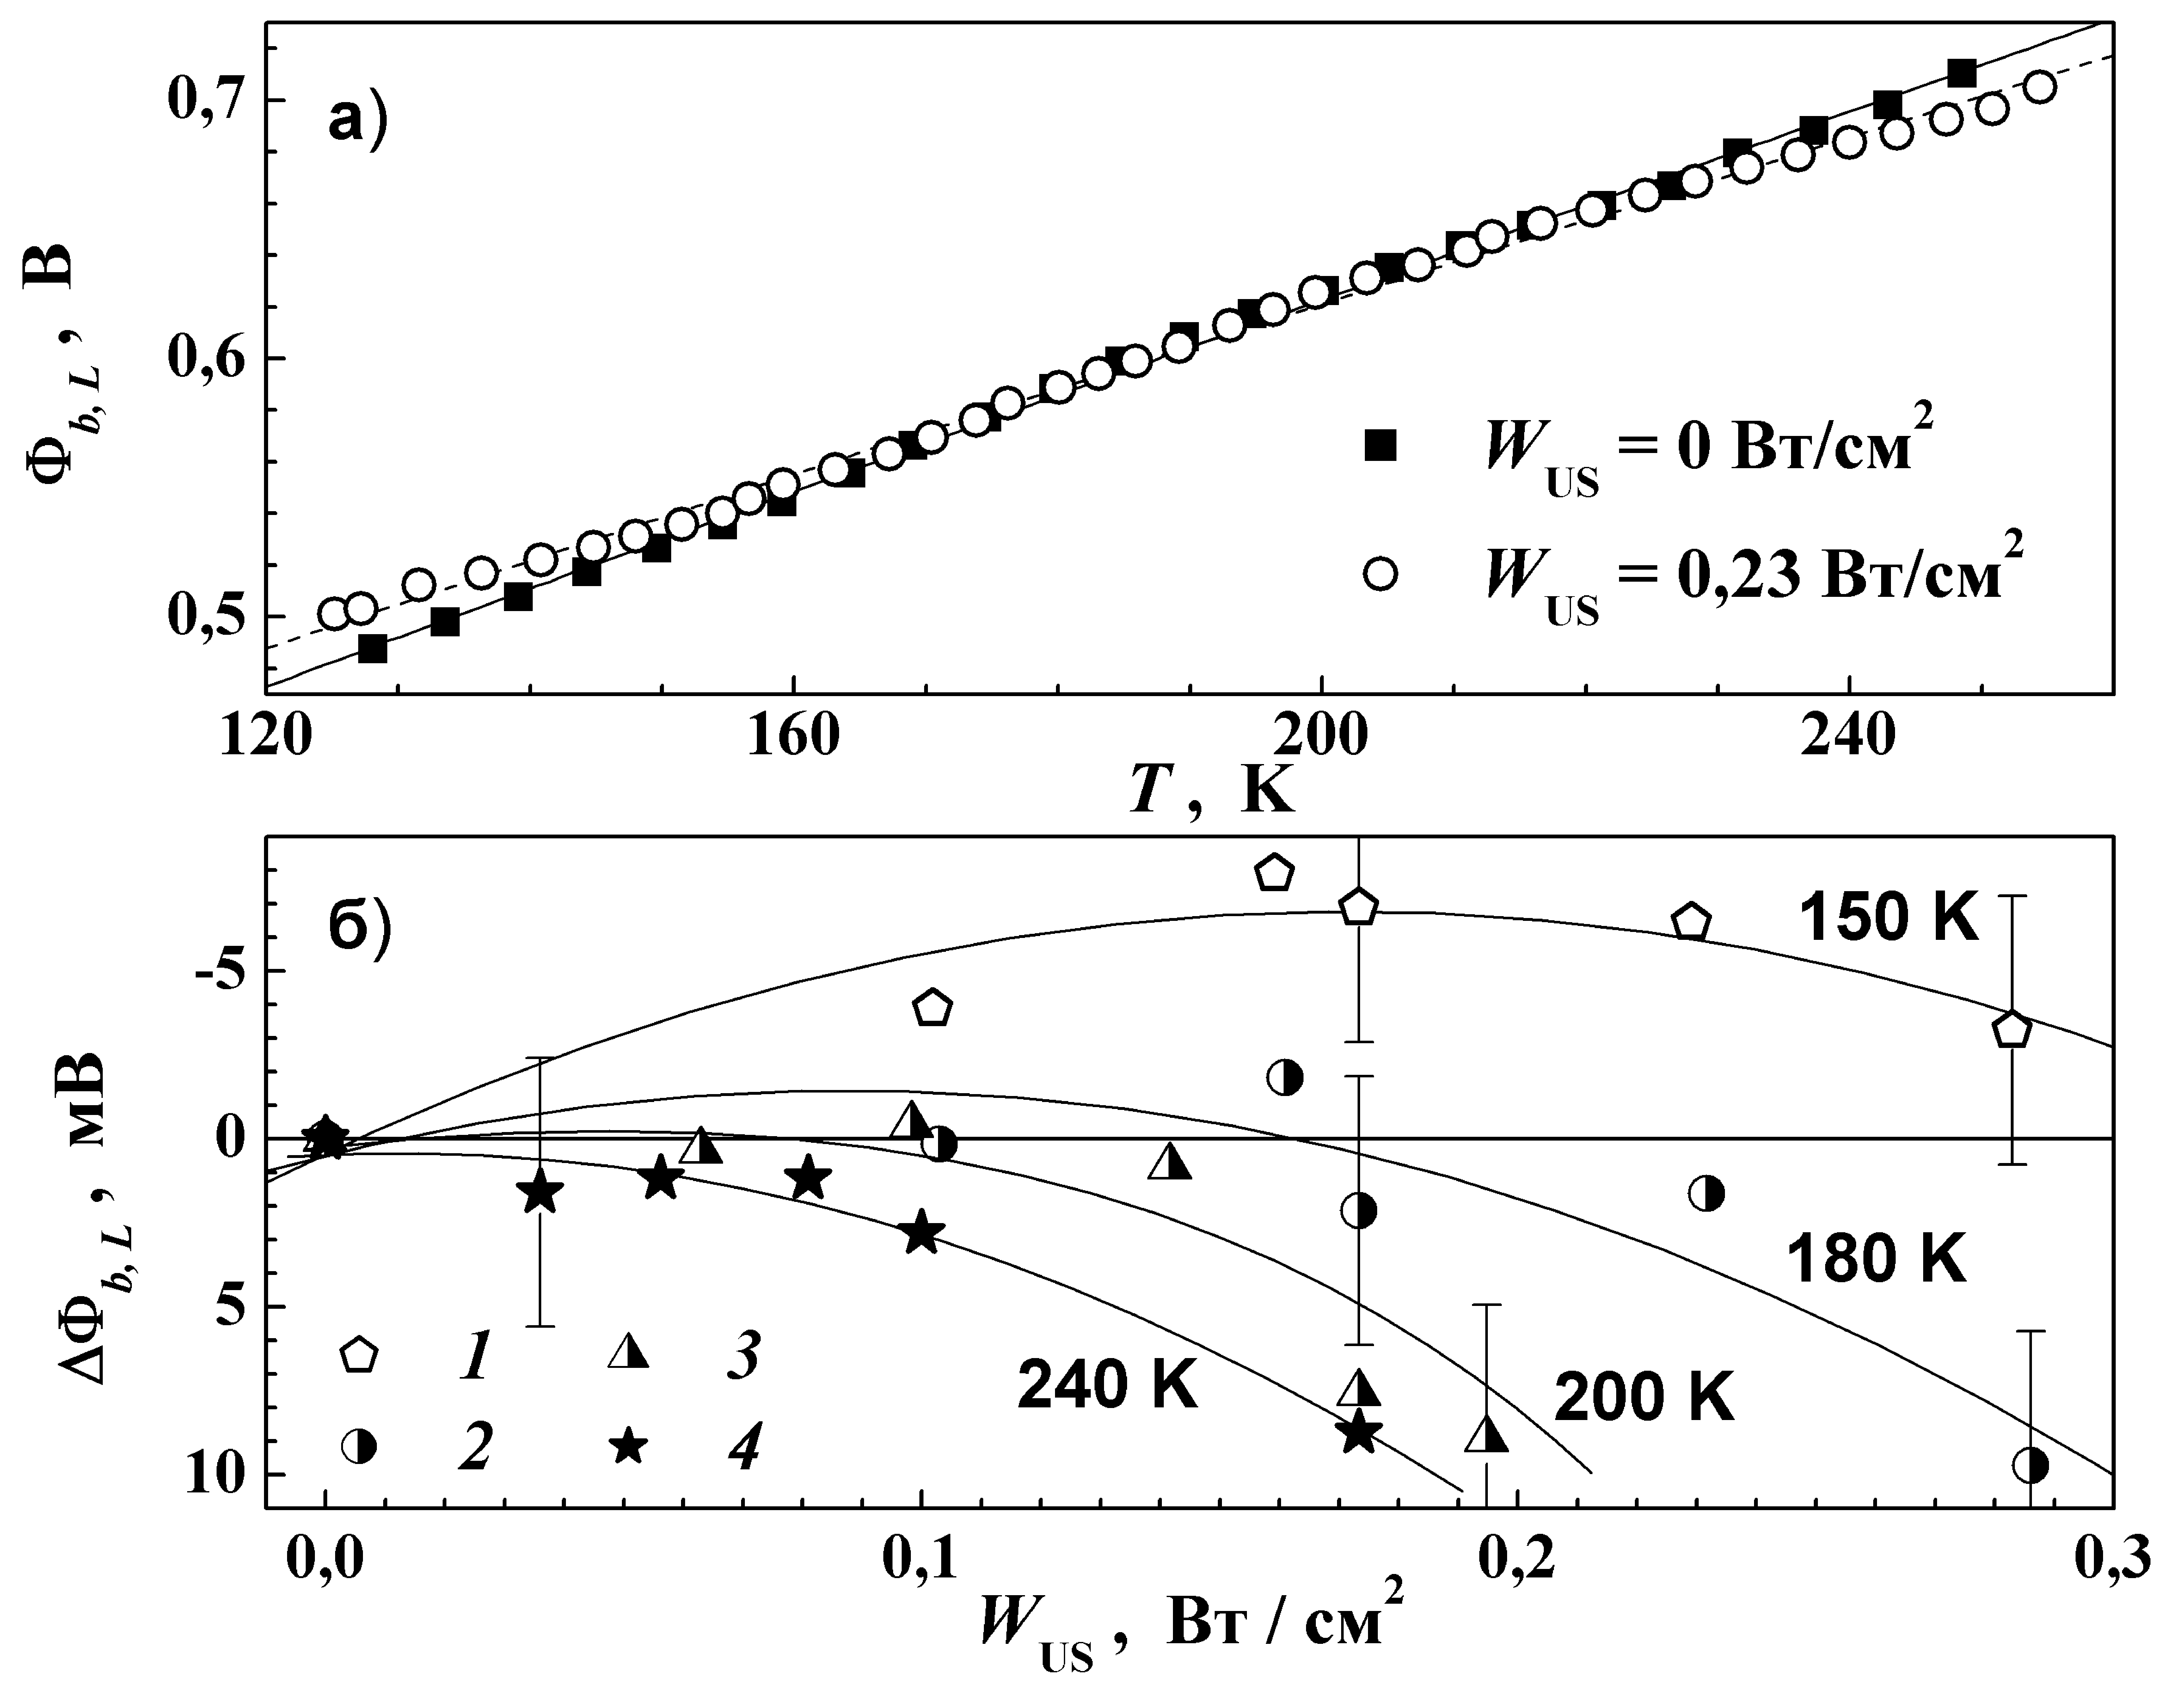
\includegraphics[width=0.9\textwidth]{figFbL_SDB}
\caption{\label{figFbL_SDB}
(a) Температурні залежності висоти бар'єру НТКС структур SSDB за умов U8SDB та без УЗН.
Лінії --- апроксимація за формулою~(\ref{eqFpApr}) (суцільна --- без УЗН).
(б) Залежності АІ змін висоти бар'єру від інтенсивності УЗ.
$T$, K: 150 (1), 180 (2), 200 (3), 240 (4).
}%
\end{figure}

Загалом, присутність подвійного вигину на ВАХ в напівлогарифмічному масштабі (див. Рис.~\ref{figIV_SDB}),
за наявності якого структура з контактом Шотки може розглядатися як два паралельно з'єднані діоди, пояснюється наявністю неоднорідностей на інтерфейсному контакті.
Відповідно до теорії Tung \cite{Tung:PhysRev,Tung:MSE},
при низьких температурах та малих зміщенях струм переважно протікає через декілька ділянок з найменшою висотою бар'єру і можуть бути виділені дві окремі компоненти струму.
В цьому випадку очікується, що при малих зміщеннях фактор неідеальності має бути досить високим.
Експериментально визначені значення $n_L$ змінюються від 2 (при 130~K) до 1.55 (при 230~K).
Для апроксимації відповідної залежності в температурному інтервалі $130\div230$~K була використана формула (\ref{eqN_T:TE});
отримані значення $T_{0,L}$ наведено в Таблиці~\ref{tabSDBPar}.
Крім того, очікується \cite{Tung:PhysRev,Tung:MSE}, що для НТКС мають бути суттєвими омічні ефекти.
Зокрема в літературі  \cite{Gammon2013} показано, що вплив послідовного опору збільшується зі зменшенням температури.
Всі зазначені особливості спостерігаються на ВАХ структур SSDB --- див. Рис.~\ref{figIV_SDB},
Це, на нашу думку, є доказом того, що НТКС пов'язана з проходженням носіїв в області патчів.


В теорії \cite{Tung:PhysRev} показано, що струм насичення НТКС може спрощено бути записаний у наступному вигляді:
\begin{equation}
\label{eqIp}
I_s=AA^*\,T^2\frac{4C_p\,\pi\,\gamma_p\,\eta_b^{2/3}kT}{9V_{bb}^{2/3}q}\cdot
\exp\left\{-\frac{q\left[\,\Phi_{b}^0-\gamma_p (V_{bb}/\eta_b)^{1/3}\right]}{kT}\right\},
\end{equation}
де
$C_p$ --- густина патчів,
$\eta_{b}=\varepsilon_s\varepsilon_0/qN_d$.
Як випливає з виразів (\ref{eqFb:TE}) та (\ref{eqIp})
\begin{equation}
\label{eqFpApr}
\Phi_{b,L}=\Phi_{b}^0-\frac{\gamma_p V_{bb}^{1/3}}{\eta_b^{1/3}} -\frac{kT}{q}\ln\left(\frac{4C_p\,\pi\,\gamma_p\,\eta_b^{2/3}kT}{9V_{bb}^{2/3}q}\right).
\end{equation}
Експериментально отримана температурна залежність $\Phi_{b,L}$ були апроксимована з використанням формули~(\ref{eqFpApr}).
При цьому $\gamma_p$ та $C_p$ розглядалися як шукані параметри,
вважалося, що температурна залежність $\Phi_{b}^0$ описується виразом (\ref{eqFbT}), а величина $\Phi_{b}^0$ при нульовій температурі
співпадає з $\Phi_{b,1}^0(0)$.
Результати апроксимації представлені на Рис.~\ref{figFbL_SDB} та в Таблиці~\ref{tabSDBPar}.

\begin{figure}
\center
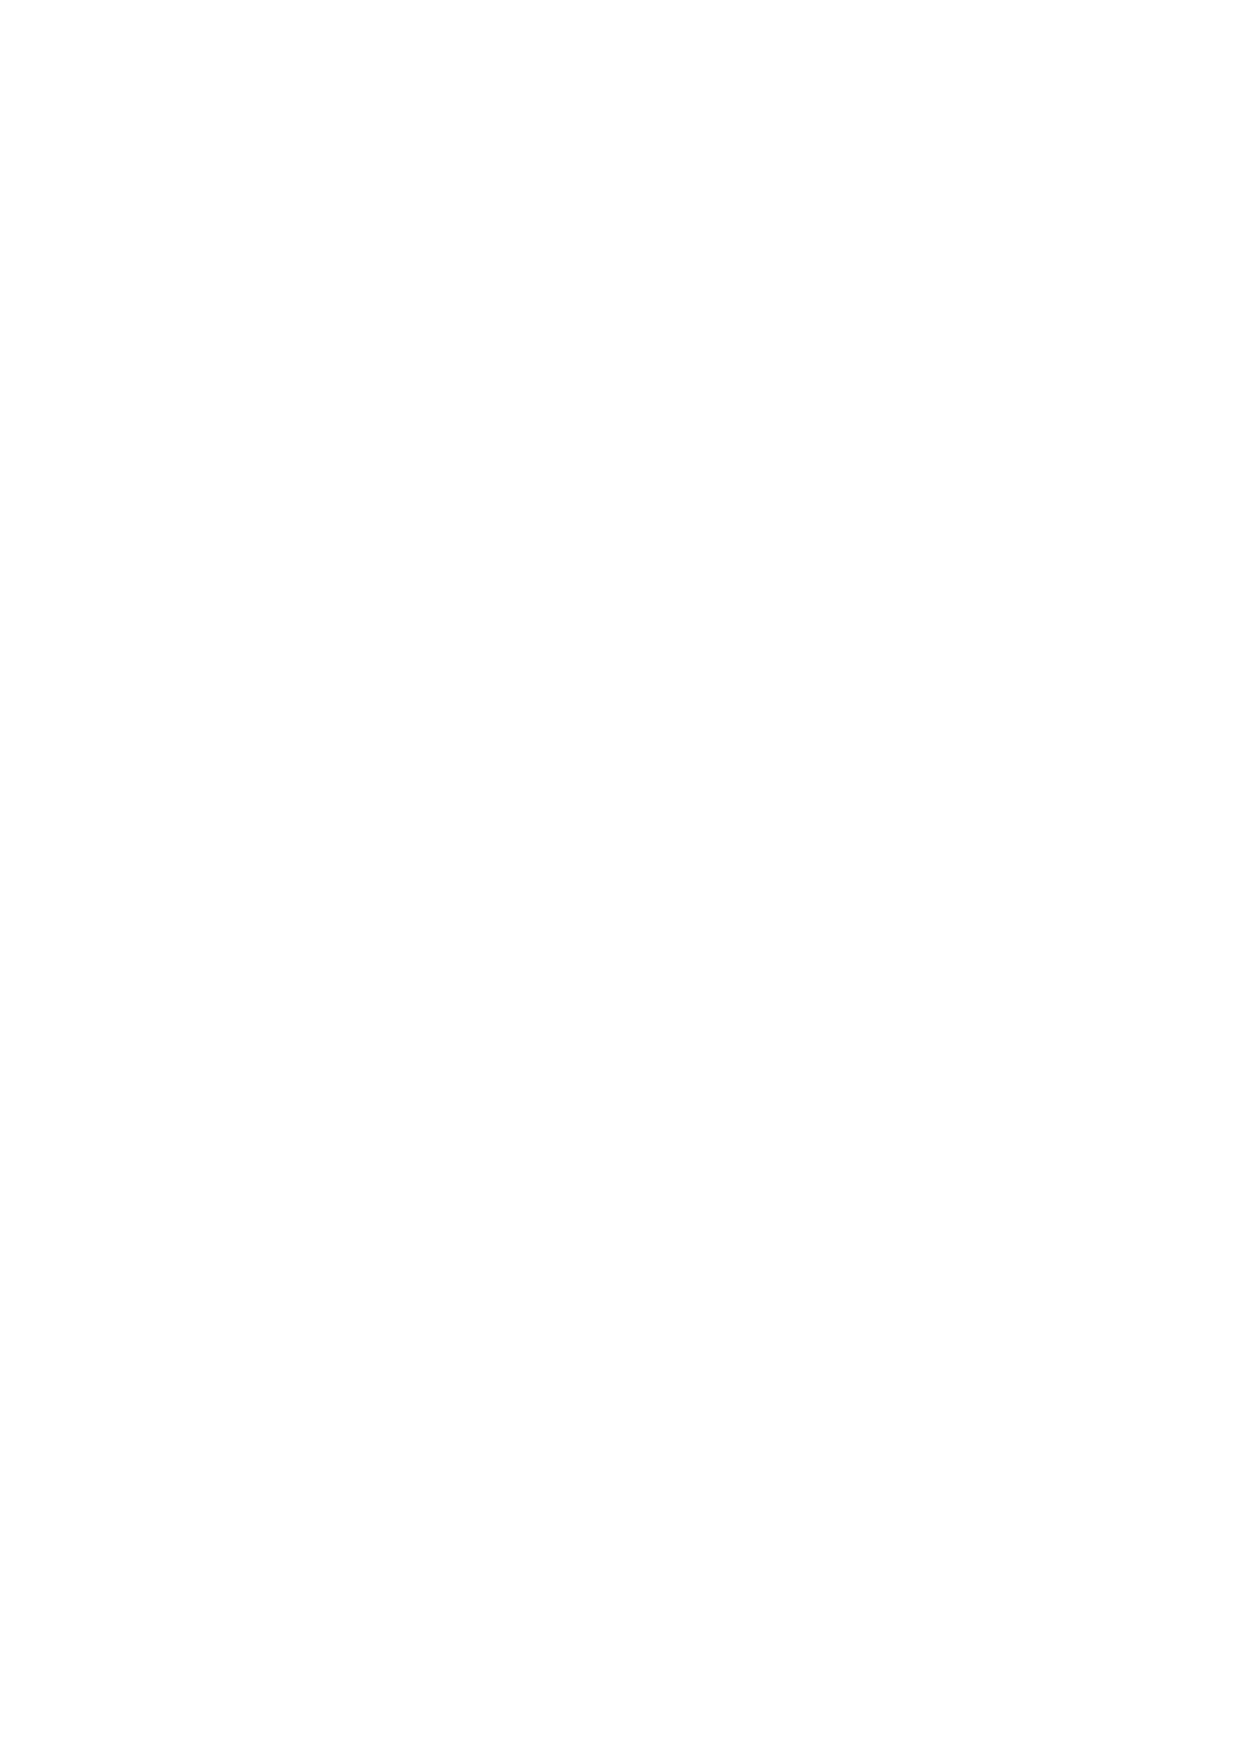
\includegraphics[width=0.75\textwidth]{figBand}
\caption{\label{figBand}
Схематичне зображення зони провідності,
що відображає різницю між випадком УЗН (верхня площина та верхня контурна поверхня) та
його відсутністю (нижня площина та нижня контурна поверхня).
Рисунок зроблено у припущенні, що наявні два патчі.
При розрахунку потенціальних поверхонь була використана формула~(1.5.3) з \cite{Tung:MSE}.
}%
\end{figure}

Проведені оцінки показують,
що в умовах УЗН величина $C_p$ суттєво (практично на порядок) зростає.
На нашу думку, причиною появи патчів в досліджених структурах є дислокації невідповідності і збільшення їх ефективної густини, як і ефективного значення розміру $R_p$,
пов'язане з коливним рухом патчів у акустичному полі.
У літературі \cite{GELCZUK2014} і раніше повідомлялося, що причиною появи неоднорідностей можуть бути саме дислокації.
З іншого боку, виявлено, що $\gamma_p$ під дією УЗ зменшується.
Це є свідченням того, що висота бар'єру в області патчів збільшується (зменшується значення $\Delta_p$).
Таким чином, відбувається згладжування потенціалу на границі розділу у полі деформацій, викликаних поширенням АХ.

Подібні оборотні АІ ефекти раніше спостерігалися в CdHgTe \cite{Vlasenko2000r}.
Авторами \cite{Vlasenko2000r} запропоновано, що точкові дефекти, локалізовані на (або біля) протяжних дефектів, внаслідок поглинання УЗ переходять в об'єм кристалічної матриці,
що стає причиною часткового вирівнювання екстремумів потенціального рельєфу.
В нашому  випадку причиною подібних ефектів може бути рух дислокаційних перегинів --- більш детально можливий механізм розглянуто у наступному параграфі.

Збільшення висоти бар'єру в області патчів може бути причиною АІ зростання $\Phi_{b,L}$ НТКС при низьких температурах.
Водночас, при збільшенні як температури, так і пружних напруг, пов'язаних з УЗ,
дислокаційні відрізки починають відриватися від точок закріплення
 і густина патчів зростає більш ефективно.
Як наслідок, ефект збільшення висоти бар'єру компенсується і $\Phi_{b,L}$ зменшується --- див. Рис.~\ref{figFbL_SDB},б.


Основні виявлені особливості впливу УЗН (збільшення висоти бар'єру за межами патчів, згладжування потенціальних неоднорідностей в області патчів) якісно показані на Рис.~\ref{figBand}.





\subsection{Особливості акусто--дефектної взаємодії у кремнієвих діодах Шотки}

Як вже згадувалося раніше, для пояснення АІ ефектів у неп'єзоелектричних кристалах
запропоновано чимало механізмів \cite{Pavlovich,Korotchenkov1995,MirzadeJAP2011,PELESHCHAK:UPJ2016,Krevchik,MirzadeJAP2005,Davletova2008,OstrovKor92},
які описують взаємодію пружних хвиль як з точковими, так і з протяжними дефектами.
Для досліджених структур процеси перенесення заряду пов'язані з термоелектронною емісією
через бар'єр, який характеризується наявністю латеральних неоднорідностей, пов'язаних з дефектами
кристалічної структури, зокрема з дислокаціями.
Отже, вплив УЗН на електричні параметри ДШ Mo$/n-n^+$--Si також доцільно розглядати саме з точки зору
взаємодії АХ з лінійними дефектами (патчами), якими, на нашу думку, є дислокації невідповідності, що
виникла внаслідок суттєвої різниці рівнів легування підкладки та епітаксійного шару.
Зупинимось більш детально на частотній та температурній залежностях зміни висоти бар'єру ВТКС,
наведеній на Рис.~\ref{figDelFbT_SDB}.
З рисунка видно, що
а)~незалежно від частоти УЗН, АІ зміна ВБШ є немонотонною функцією температури;
б)~температура, при якій спостерігається максимальний вплив УЗ, слабко зростає при збільшенні $f_\mathtt{US}$.

\begin{figure}
\center
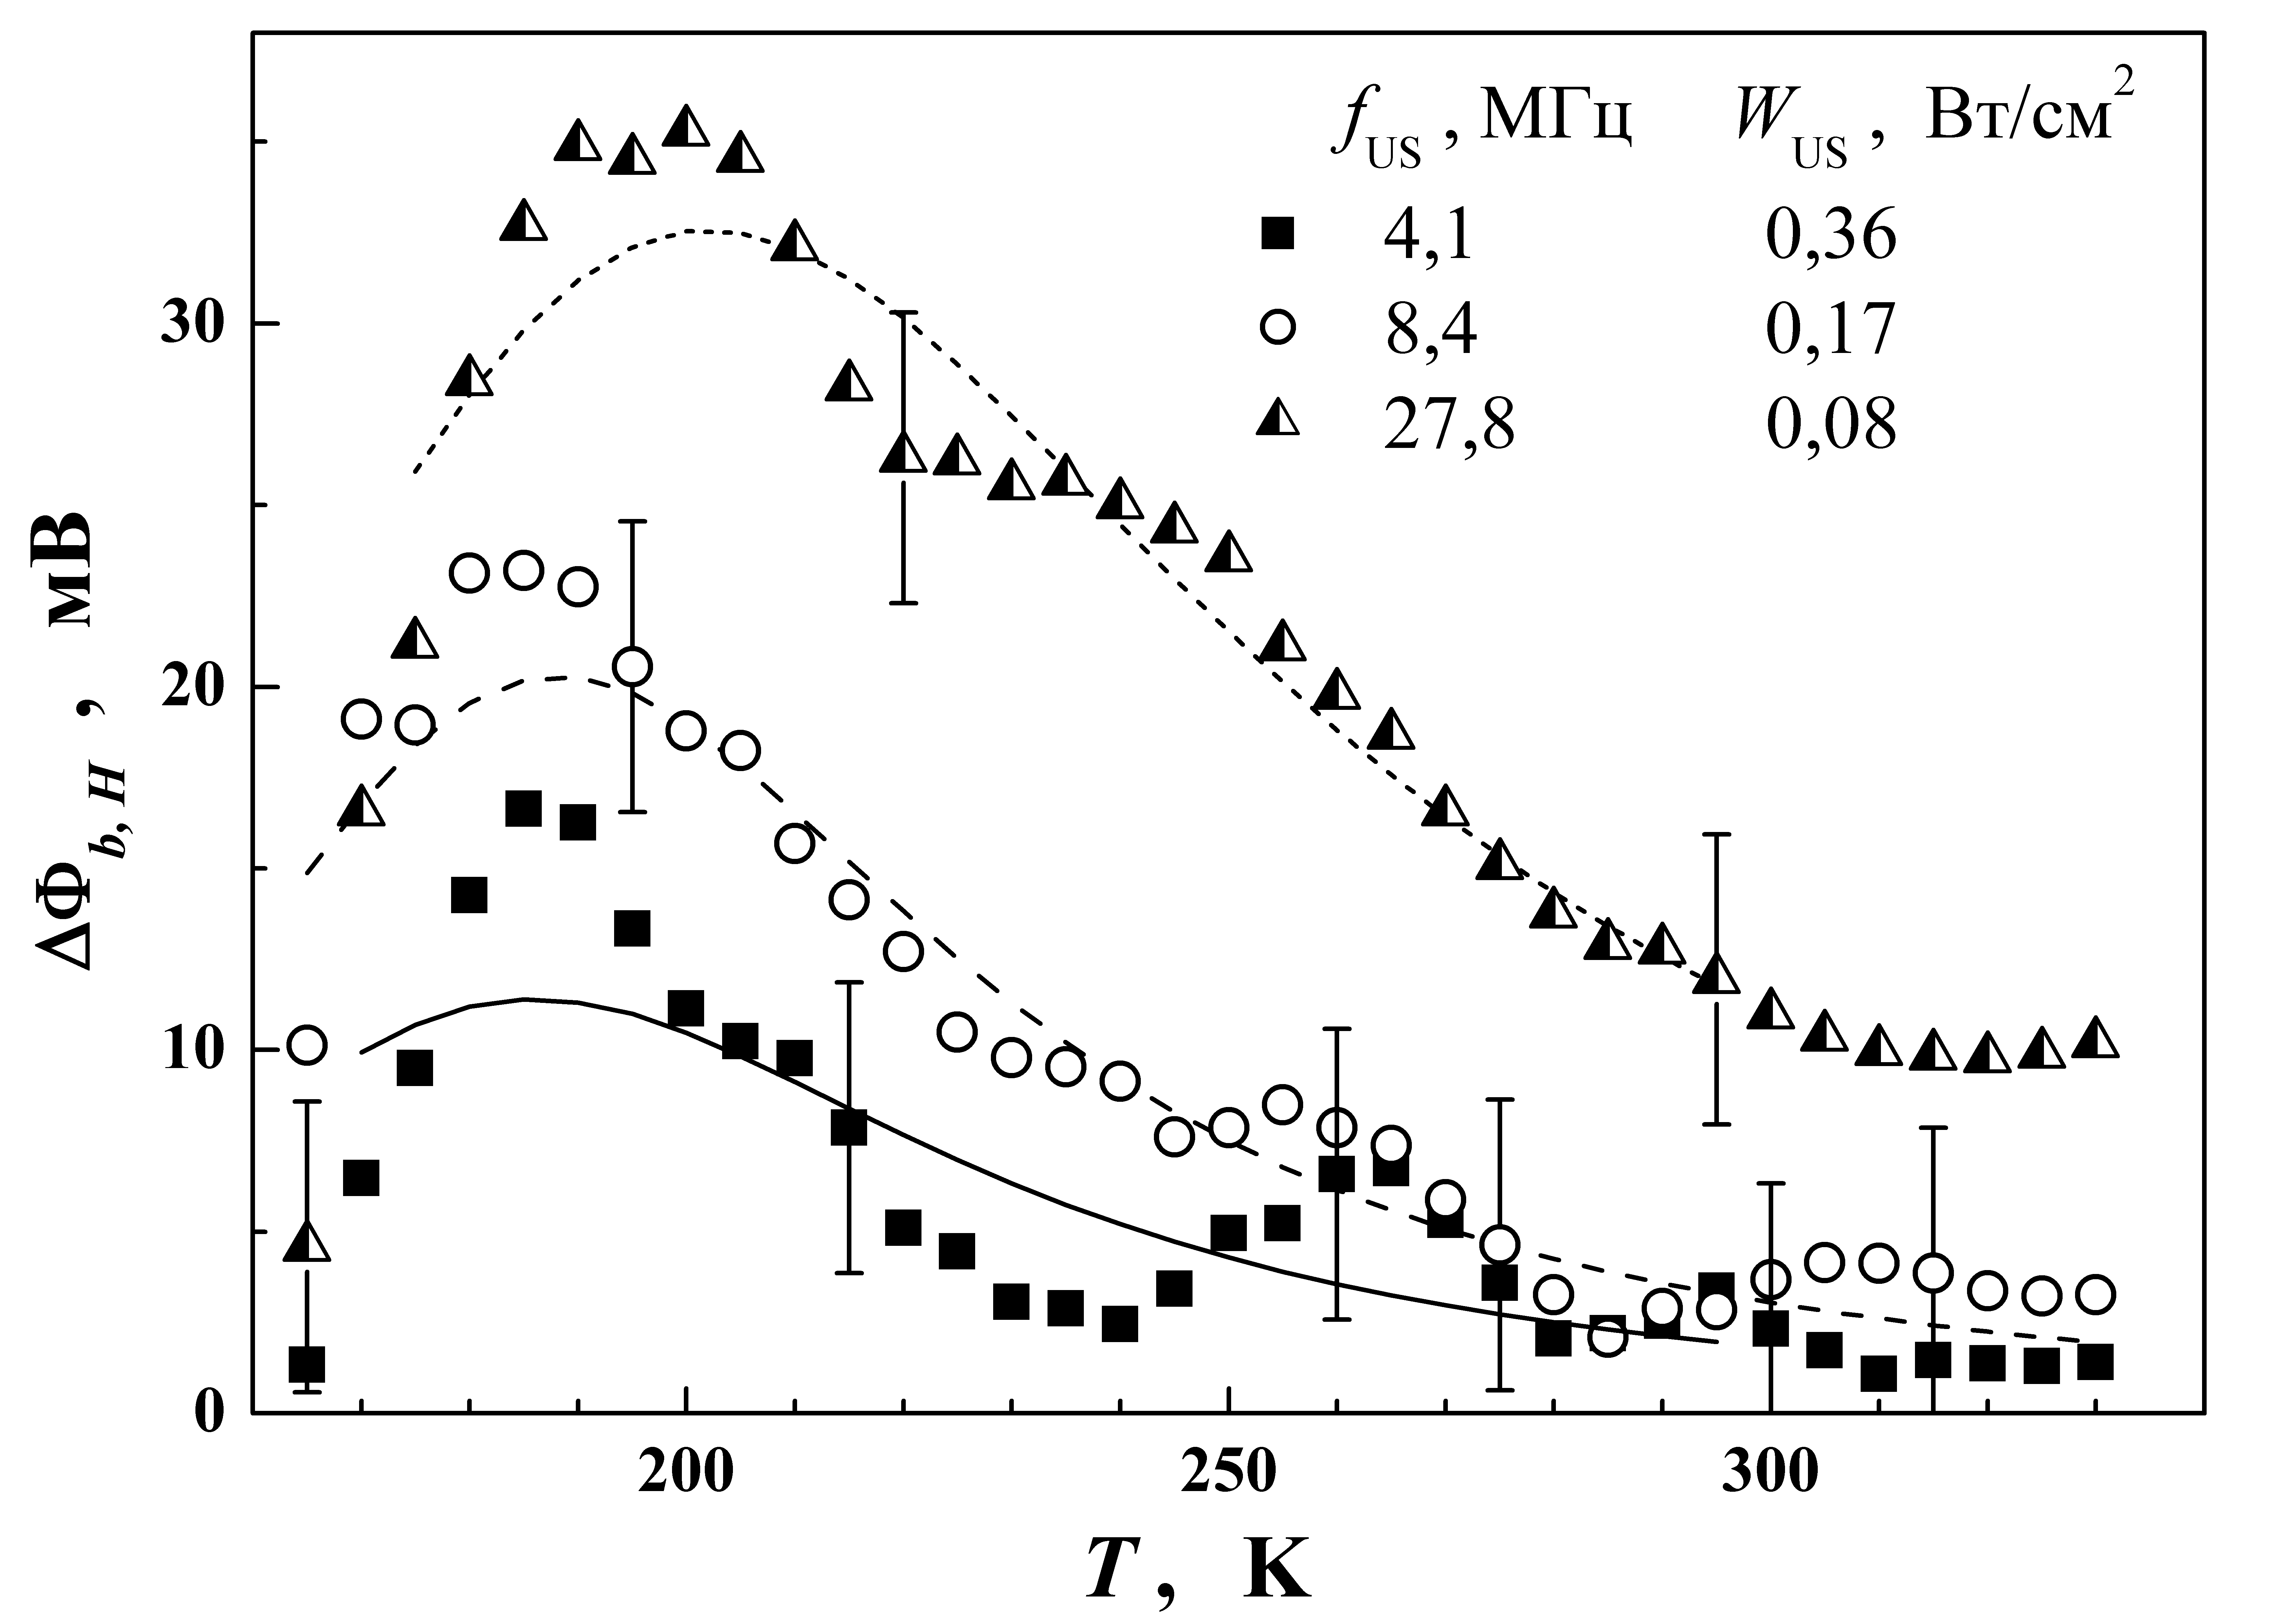
\includegraphics[width=0.7\textwidth]{figDelFbT_SDB}
\caption{\label{figDelFbT_SDB}
Температурні залежності змін ВБШ при УЗН з різними частотами.
Точки --- експеримент,
лінії --- апроксимація згідно з формулою~(\ref{eqBr}).
}%
\end{figure}

Амплітуда АІ змін ВБШ підвищується при введенні у зразок УЗ з більшою інтенсивністю, причому незалежно від частоти та температури
відповідні залежності близькі до лінійних.
Цей ефект ілюструється проілюстровано на Рис.~\ref{figDelFbWus_SDB}.
Отже, можна записати наступне співвідношення
\begin{equation}
\label{eqBt}
\Delta\Phi_{b,H}\,(f_\mathtt{US},\,T)=\beta_\mathtt{US}\,(f_\mathtt{US},\,T)\cdot W_\mathtt{US},
\end{equation}
де
$\beta_\mathtt{US}$ характеризую частку енергії АХ, витрачену на зміну ВБШ, або, іншими слова,
ефективність впливу УЗ на висоту бар'єру Шотки.
З Рис.~\ref{figDelFbT_SDB} та \ref{figDelFbWus_SDB} видно, що при збільшенні частоти УЗ $\beta_\mathtt{US}$ також зростає.
У лінійному наближенні коефіцієнт $\beta_\mathtt{US}$ має бути пропорційним коефіцієнту поглинання АХ $\alpha_\mathtt{US}$ дислокаціями.

\begin{figure}
\center
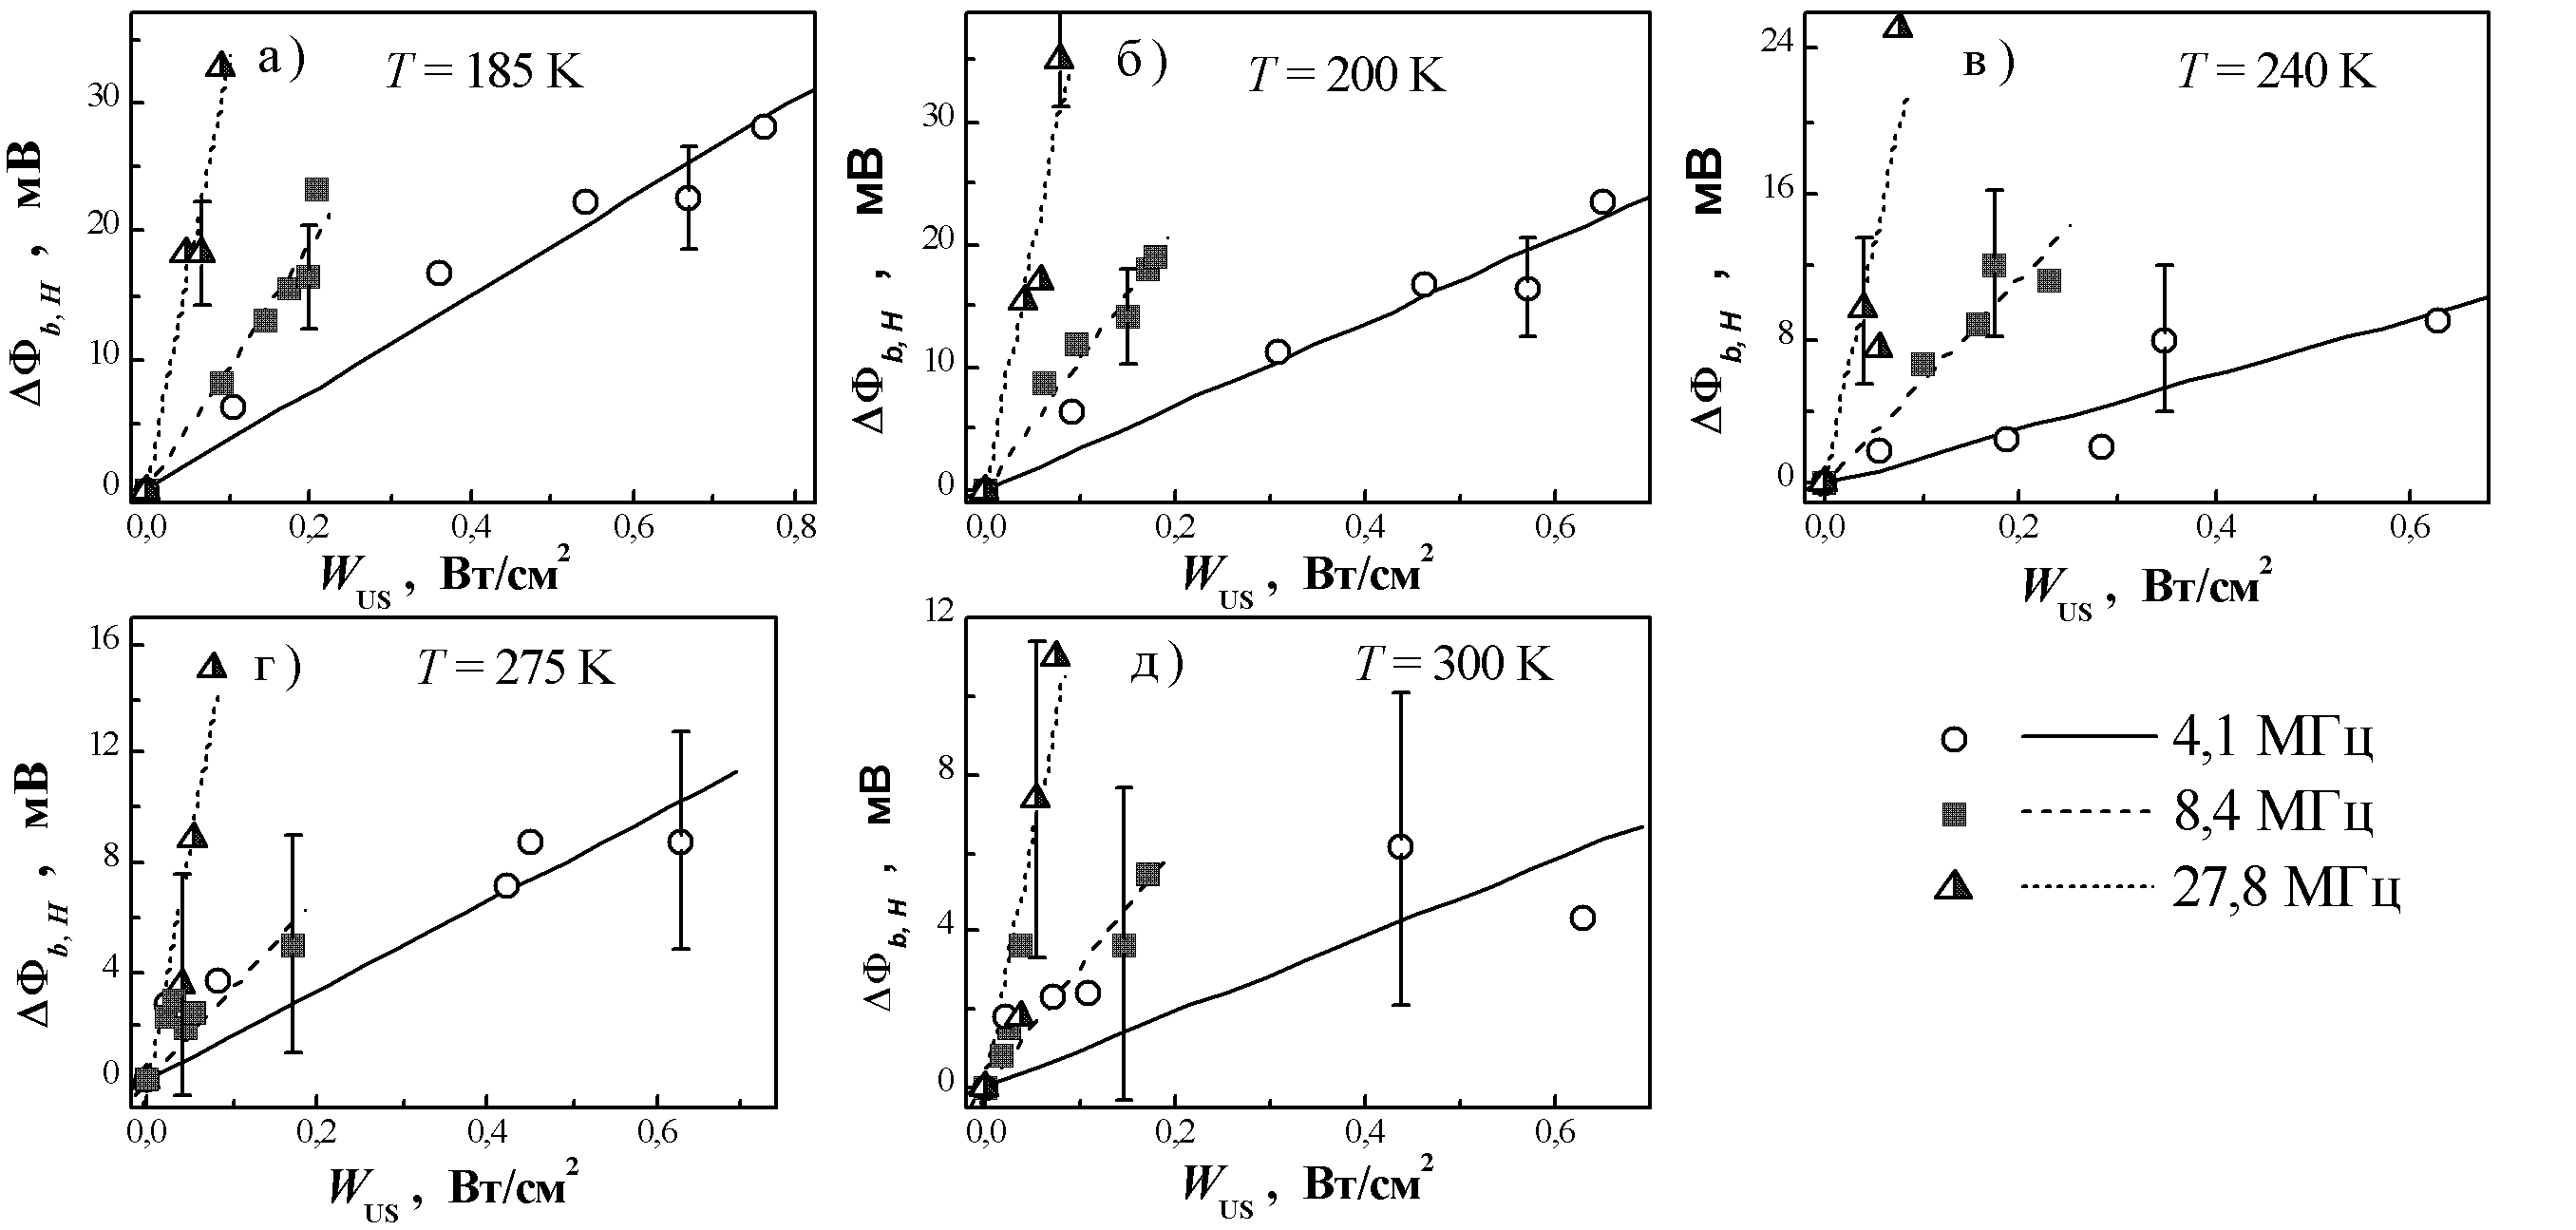
\includegraphics[width=1\textwidth]{figDelFbWus_SDB}
\caption{\label{figDelFbWus_SDB}
Залежності АІ змін ВБШ від інтенсивності введеного УЗ.
Точки --- експеримент,
лінії --- апроксимація згідно з формулою~(\ref{eqBt}).
}%
\end{figure}

Загалом, затухання об'ємних УЗ хвиль у кристалах може бути пов'язано з різними механізмами \cite{True},
зокрема з фонон--фононними процесами,
термопружними втратами, резонансним поглинанням на мало--кутових границях субблочних кристалів чи дислокаційним поглинанням.
Проте, проведені оцінки показують, що в умовах експерименту (для інтервалу температур $130\div330$~K та частот $4\div28$~МГц) затухання завдяки першим двом механізмам
є досить незначним, тоді як мало--кутові границі у монокристалічних досліджених структурах відсутні зовсім.
Щодо дислокаційного поглинання, то чи найвідомішим наближенням, яка описує подібні процеси є модель Гранато--Люкке.
Незважаючи на те, що це модель дислокаційного тертя була розвинута в ідеалізованому наближенні нульової температури кристала, вона успішно застосовується для аналізу
дислокаційного поглинання у різних реальних матеріалах, зокрема і у напівпровідникових кристалах \cite{OstrKorBook,Nik}.
При такому підході дислокація розглядається як струна, закріплена в певних точках, причому вільні відрізки між точками закріплення можуть вимушено коливатися під дією зовнішньої сили, зокрема, пов'язаної з поширенням ультразвуку.
 Коефіцієнт поглинання акустичної хвилі при малих частотах $\omega_\mathtt{US}=2\pi f_\mathtt{US}<<\omega_\mathtt{dis}$
(де $\omega_\mathtt{dis}$ --- власна частота коливань дислокаційного відрізку, яка залежить від його довжини та пружних модулів кристалу)
 має описуватися наступним співвідношенням \cite{Granato,True}:
\begin{equation}
\label{eqAlphsGL}
\alpha_\mathtt{US}=\frac{4G\rho_\mathtt{dis}\omega_\mathtt{US}^2}{\upsilon_\mathtt{Si}\pi^3\rho_\mathtt{Si}}\cdot
    \frac{d}{(\omega_\mathtt{dis}^2-\omega_\mathtt{US}^2)^2+d^2\omega_\mathtt{US}^2}\,,
\end{equation}
де $G$ --- модуль зсуву,
$d = B/(\pi\rho_\mathtt{Si} b^2)$ -- стала демферування;
$B$ --- коефіцієнт динамічної в'язкості;
$b$ --- модуль вектора Бюргерса.

Як показують розрахунки, $\alpha_\mathtt{US}$ має досягати максимального значення при
$d_\mathtt{max}=(\omega_\mathtt{dis}^2 - \omega_\mathtt{US}^2)/\omega_\mathtt{US}$.
При цьому:
\begin{equation}
\label{eqAlGLmax}
\alpha_\mathtt{US,max}=\frac{2G\rho_\mathtt{dis}\omega_\mathtt{US}}{\upsilon_\mathtt{Si}\pi^3\rho_\mathtt{Si}(\omega_\mathtt{dis}^2-\omega_\mathtt{US}^2)}
\approx\frac{2G\rho_\mathtt{dis}\omega_\mathtt{US}}{\upsilon_\mathtt{Si}\pi^3\rho_\mathtt{Si}\omega_\mathtt{dis}^2}\,,
\end{equation}
тобто $\alpha_\mathtt{US,max}$ має бути пропорційна частоті УЗ,
так як резонансна частота коливань дислокаційного відрізку не повинні залежати від частоти зовнішнього збурення.
Очікуване згідно з теорією Гранато--Люкке зростання $\alpha_\mathtt{US}$ та $\alpha_\mathtt{US,max}$ з підвищенням $\omega_\mathtt{US}$ загалом
збігається з експериментально отриманою поведінкою коефіцієнта $\beta_\mathtt{US}$.

Щодо температурної поведінки коефіцієнта поглинання, то мусимо зауважити наступне.
З літератури \cite{Si_C:Temp} відомо, що зміни пружних модулів кристалів Si у температурному діапазоні, де проводилися дослідження, не перевищують $(1\div2)\%$.
Якщо припустити, що $\omega_\mathtt{dis}$ та $\rho_\mathtt{Si}$ також слабо залежать від температури, то, згідно з \eqref{eqAlphsGL}, температурна залежність $\alpha_\mathtt{US}$ має визначатися змінами параметру $d$, тобто, фактично, коефіцієнтом динамічної в'язкості.
В рамках даної моделі передбачається, що гальмування руху дислокацій, у тому числі і коливального в УЗ полі,
відбувається завдяки їх взаємодії з фононами, носіями заряду, а також за рахунок термопружних втрат \cite{Granato,Sudz,True}.
Температурна залежність кожного з цих механізмів, а також їх відносні внески у величину $B$ та $d$ можуть суттєво залежати від матеріалу і тому точно описати залежність $\alpha_\mathtt{US}(T)$ в рамках моделі Гранато-Люкке досить складно.
Проте у багатьох роботах, зокрема в \cite{True}, було показано, що в області  температур,
які відповідають нашим експериментам, величина $B$ практично лінійно зростає з підвищенням $T$.
Таким чином, з врахуванням того, що використані частоти УЗН набагато менші $\omega_\mathtt{dis}$, коефіцієнт поглинання має монотонно збільшуватися при зростанні температури.
Така залежність, зокрема, була експериментально зафіксована в роботі \cite{YOlikh:USadsorb} у кристалах нейтронно--легованого кремнію при $T=100\div300$~К.
Проте в нашому випадку залежності АІ змін від температури характеризуються наявністю максимуму, а отже
модель Гранато--Люкке не може бути повністю використана для пояснення виявлених ефектів зміни ВБШ.

З іншого боку, в літературі \cite{Brailsford} також представлена модель, запропонована Брейсфолдом для пояснення характерних піків поглинання акустичних хвиль, які спостерігалися у пластично-деформованих металах при низьких температурах.
Згідно з цією моделлю дислокація розглядається як послідовність сегментів, орієнтованих у напрямі щільного пакування та з'єднаних різкими перегинами.
Дислокація вважається жорстко закріпленою у кінцевих точках, а поглинання УЗ здійснюється за рахунок стимулюваного переміщення перегинів.
Припускається, що дифузія перегинів має термоактиваційний характер і коефіцієнт дифузії $D_k$ описується виразом
\begin{equation}\label{eqDkink}
  D_k = D_{0k} \exp\left(-\frac{W_k}{kT}\right),
\end{equation}
де $W_k$ --- енергія активації дифузії,
$D_{0k}$ --- певна константа.
Причому між $f_\mathtt{US}$ та температурою, при якій спостерігається максимум поглинання $T_\mathtt{max}$, має існувати зв'язок:
\begin{equation}
\label{eqfk}
f_\mathtt{US}=f_k\exp\left(-\frac{W_k}{kT_\mathtt{max}}\right)\,,
\end{equation}
де
$f_k=\pi D_{0k}/(20 \,l_0^2)$ --- певний параметр, пов'язаний з середньою довжиною дислокаційного сегменту $l_0$.

Згідно з \cite{Brailsford} добротність $Q_l$, яка пов'язана з поглинанням АХ одним дислокаційним сегментом довжиною $l$, має описуватися виразом:
\begin{equation}
\label{eqQl}
Q_l^{-1}=\frac{8Ga^2b^2l^3(n_{0k}+p_{0k})}{V_vkT\pi^4}\cdot
\frac{\left(\frac{\omega_\mathtt{US} l^2}{20\pi l_0^2f_k}\right)\exp{\left(\frac{W_k}{kT}\right)}}
{1+\left(\frac{\omega_\mathtt{US} l^2}{20\pi l_0^2f_k}\right)^2\exp{\left(\frac{2W_k}{kT}\right)}}\,,
\end{equation}
де $a$ --- стала ґратки,
$n_{0k}$ та $p_{0k}$ --- рівноважні лінійні концентрації правих та лівих перегинів, відповідно;
$V_v$ --- об'єм кристалу.
В теорії передбачено, що для оцінки загальної добротності кристалу $Q_\mathtt{US}$ необхідно
помножити загальну кількість дислокаційних сегментів $\rho_\mathtt{dis}V_v/l_0$
на усереднене з врахуванням розподілу сегментів по довжині значення $Q_l$.
У спрощеному випадку, якщо замість усереднення замінити $l$ в \ref{eqQl}
на певну ефективну довжину сегменту \mbox{$l_{eff} = g_l l_0$} та врахувати співвідношення $Q_\mathtt{US}^{-1} = \alpha_\mathtt{US}\upsilon\ln{10}/(10 \,\omega_\mathtt{US})$, то вираз, який описує поглинання згідно з моделлю Брейсфолда, набуде наступного вигляду:
\begin{equation}
\label{eqAlpaBr}
\alpha_\mathtt{US}(f_\mathtt{US},\,T)=\frac{8Ga^2b^2g_l^3D_{0k}(n_{0k}+p_{0k})\rho_\mathtt{dis}}{\ln{10}\:\upsilon_\mathtt{Si} f_k k\pi^2}\cdot Y(f_\mathtt{US},\,T)\,,
\end{equation}
де функція
\begin{equation}
\label{eqY}
Y(f_\mathtt{US},\,T)=\frac{f_\mathtt{US}}{T}\cdot\frac{\left(\frac{f_\mathtt{US} g_l^2}{10 f_k}\right)\exp{\left(\frac{W_k}{kT}\right)}}
{1+\left(\frac{f_\mathtt{US} g_l^2}{10 f_k}\right)^2\exp{\left(\frac{2W_k}{kT}\right)}}
\end{equation}
визначає, переважним чином, температурну та частотну залежності коефіцієнта поглинання.
Розрахований вигляд функції $Y(f_\mathtt{US},\,T)$ наведено на Рис.~\ref{figY_SDB}.
З рисунка видно, що загалом особливості температурних та частотних залежностей коефіцієнта поглинання УЗ співпадають
з особливостями залежностей АІ зміни ВБШ (Рис.~\ref{figDelFbT_SDB}).


\begin{figure}
\center
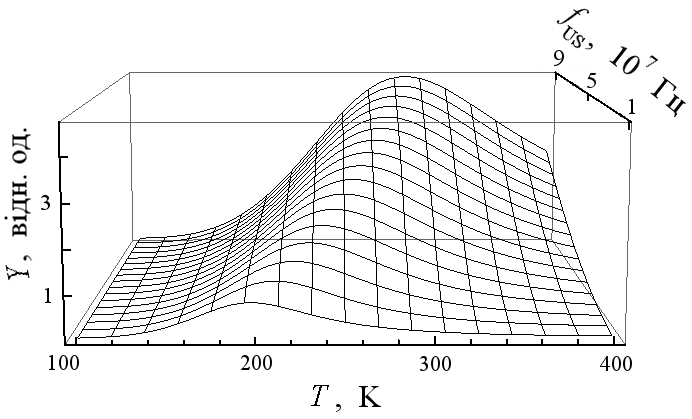
\includegraphics[width=0.6\textwidth]{figY_SDB}
\caption{\label{figY_SDB}
Температуро--частотна залежність функції $(f_\mathtt{US},\,T)$.
При розрахунках за формулою~(\ref{eqY}) вважалося, що
$W_k=0,108$~еВ, $f_k=6\cdot10^9$~Гц, $g=3,5$.
}%
\end{figure}

Враховуючи формули (\ref{eqBt}), (\ref{eqAlpaBr}) та (\ref{eqY}),
вираз що описує АІ зміни висоти бар'єру можна представити у вигляді
\begin{equation}
\label{eqBr}
\Delta\Phi_{b,H}\,(f_\mathtt{US},\,T)\sim\frac{f_\mathtt{US}}{T}\frac{(f_\mathtt{US}/{f_k})\exp\left(\frac{W_k}{kT}\right)}
{1+(f_\mathtt{US}/{f_k})^2\exp\left(\frac{2W_k}{kT}\right)}W_\mathtt{US}.
\end{equation}
При записі останнього співвідношення враховано, що
в роботі \cite{Olikh:UPJ2014} показано, що непогане узгодження експериментальних даних щодо коефіцієнта поглинання УЗ з теоретичними
досягається при $g_l=3,5$.



Вираз~(\ref{eqBr}) був використаний для апроксимації температурних залежностей АІ змін ВБШ.
Результати представлені на Рис.~\ref{figDelFbT_SDB}.
Встановлено, що достатньо високе узгодження між експериментальними даними та апроксимуючими кривими спостерігається
при  $W_k=(90\pm10)$~меВ таd $f_k=(3\pm2)\cdot10^9$~Гц.

Збільшення $\beta_\mathtt{US}$ при зростанні частоти УЗН (Рис.~\ref{figDelFbfus_SDB}) також збігається
з передбаченнями теорії Брейсфолда.
Нами були використана формула~(\ref{eqBr}) та значення $W_k=90$~меВ для апроксимації експериментально виявленої частотної залежності АІ змін ВБШ.
Результати представлені на Рис.~\ref{figDelFbfus_SDB}.


\begin{figure}
\center
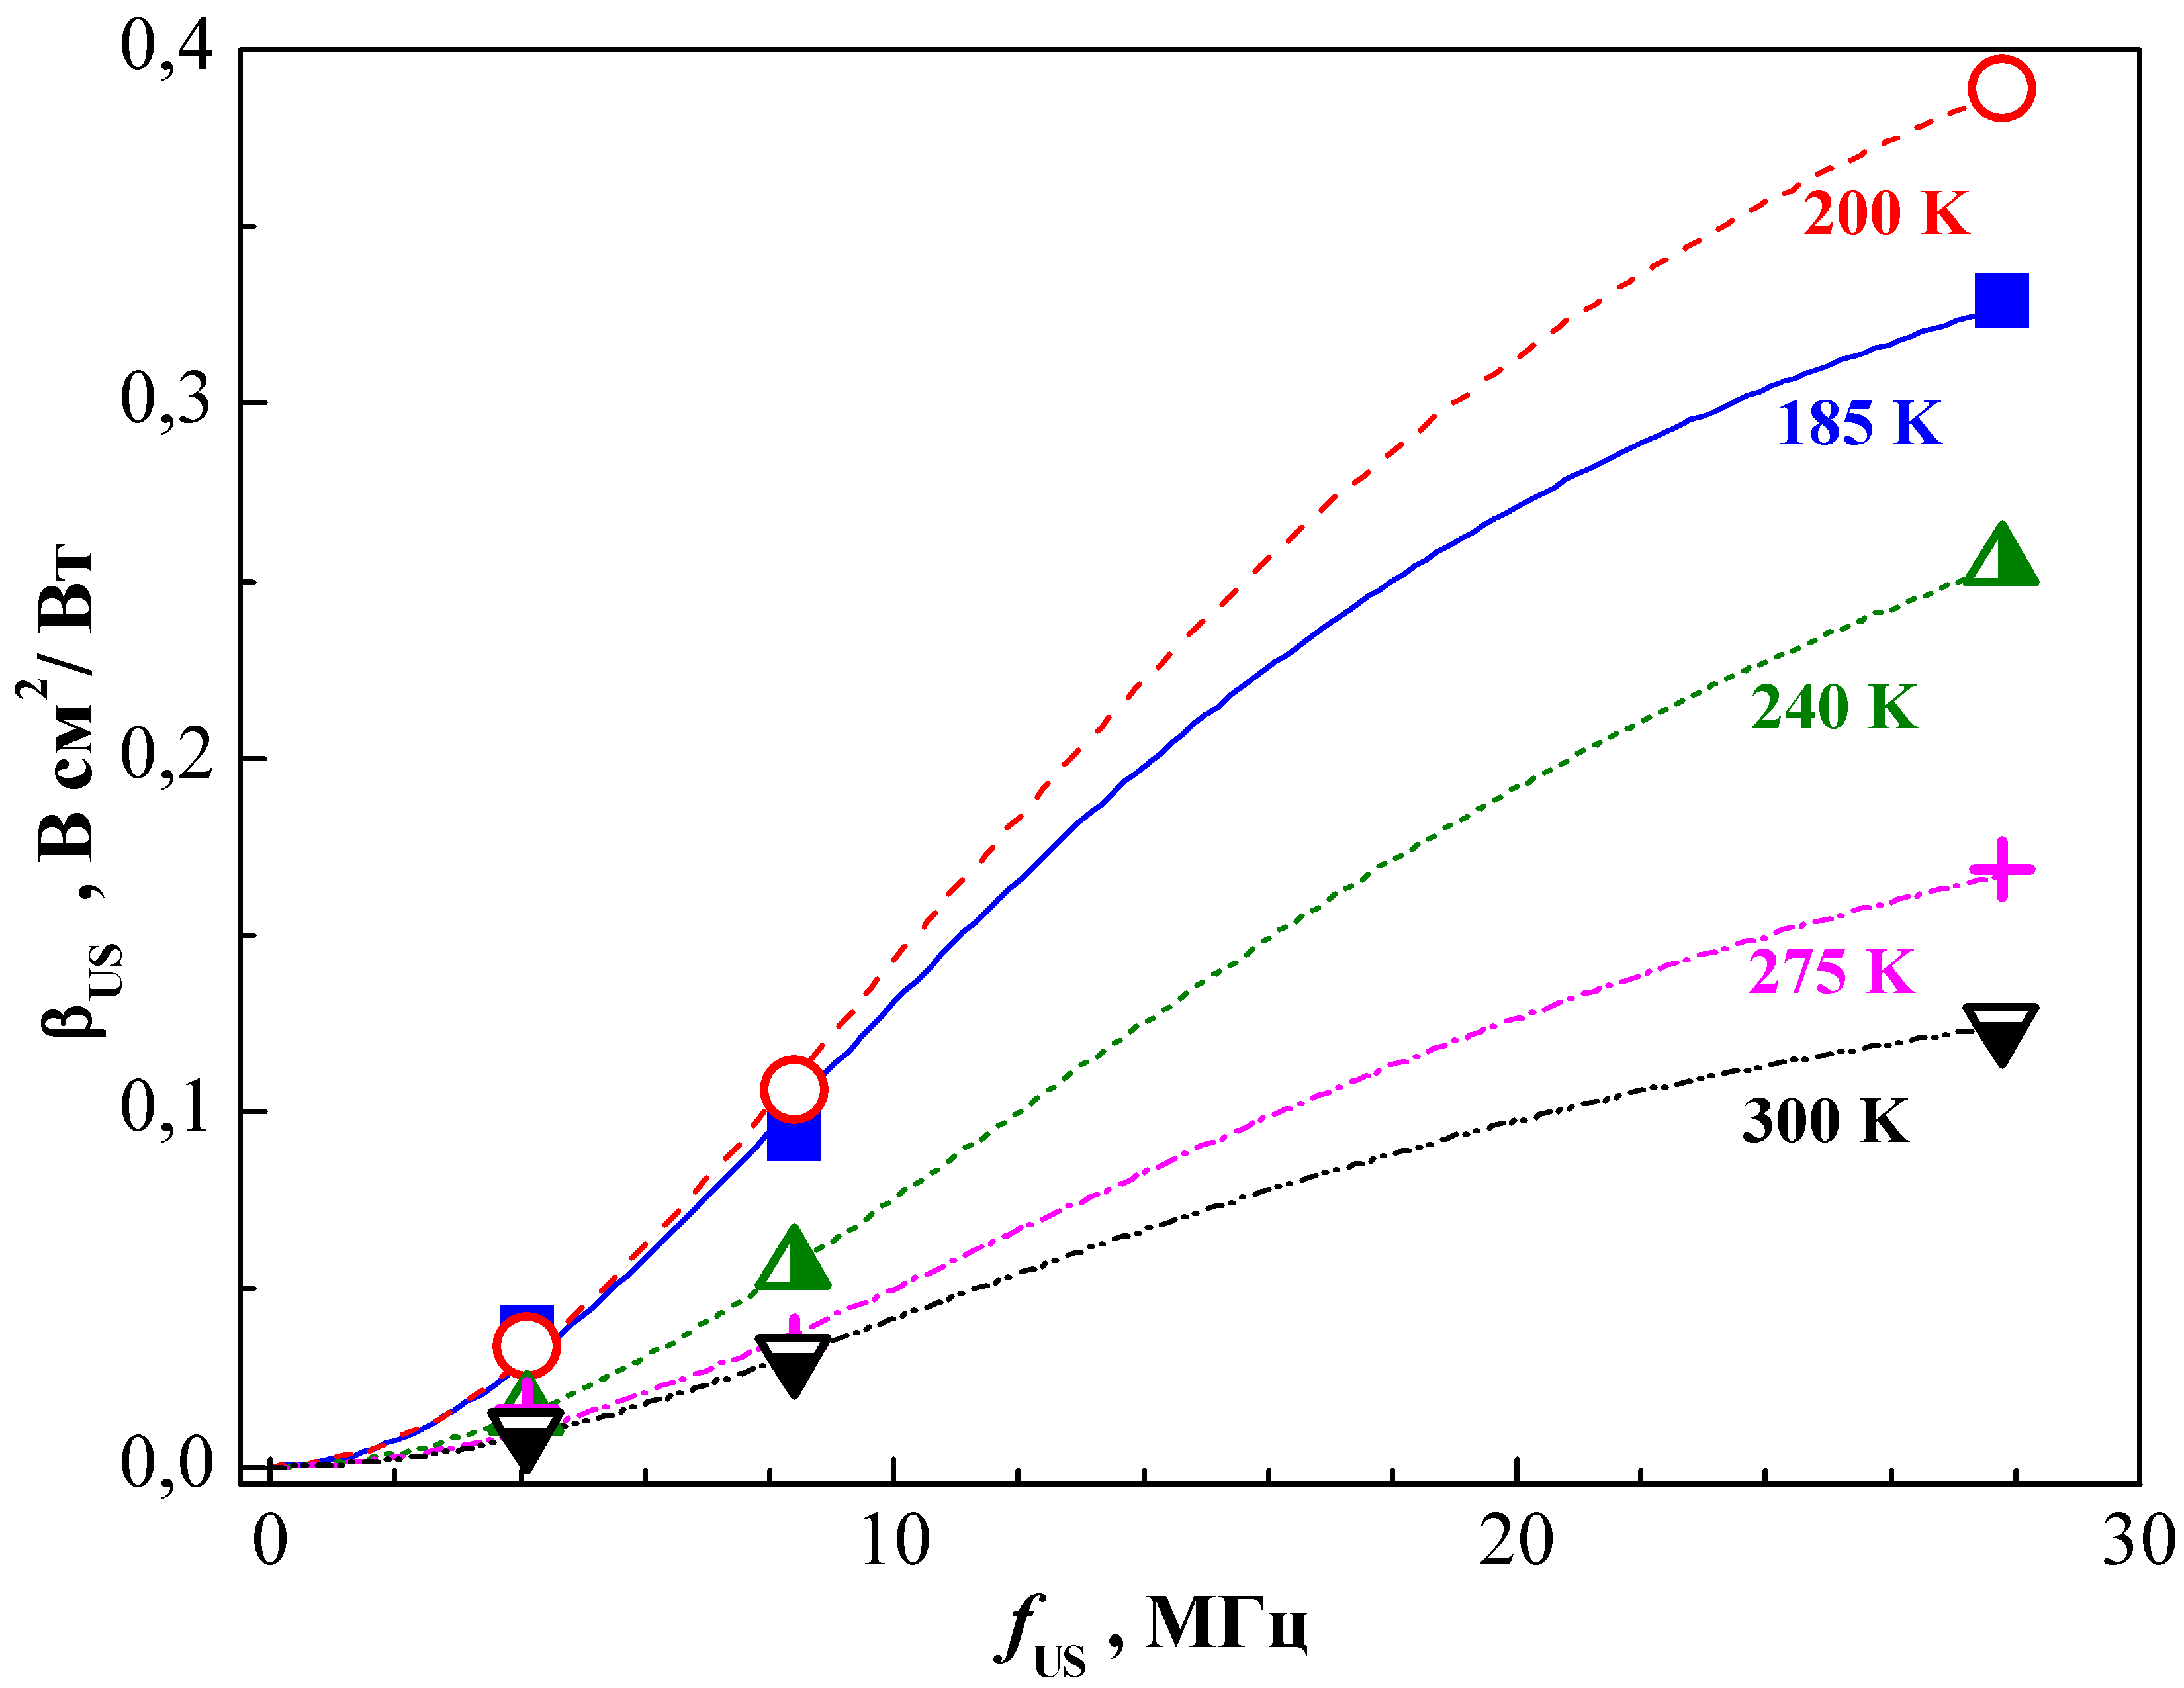
\includegraphics[width=0.65\textwidth]{figDelFbfus_SDB}
\caption{\label{figDelFbfus_SDB}
Частотні залежності ефективності впливу УЗ на висоту бар'єру при різних температурах.
Точки --- експеримент,
лінії --- апроксимація згідно з формулою~(\ref{eqBr}).
}%
\end{figure}


Таким чином, показано, що модель поглинання УЗ внаслідок руху дислокаційних перегинів цілком застосовна
для пояснення особливостей температурних та частотних залежностей динамічного АІ впливу на висоту бар'єру Шотки в структурах Mo$/n$-$n^+$--Si.
Зауважимо, що модель руху елементів тонкої структури дислокації до
пояснення АІ ефектів у напівпровідниках застосовувався і раніше.
Так, наприклад, у роботі \cite{Loktev} вона застосовується для пояснення амплітудно--залежних ефектів
під дією інтенсивної УЗ хвилі, зокрема ефекту акустолюмінісценції в CdS.


\section{Вплив ультразвукового навантаження на струм втрат діодів Шотки Mo$/n-n^+$--Si\label{SSDB:Rev}}

Струм втрат є одним з найважливіших параметрів для різноманітних напівпровідникових пристроїв, що визначає їх робочі характеристики.
Не дивно, що його вивченню приділяється чимала увага --- див., наприклад, роботи \cite{Sathaiya,VRH:Shan,Pipinys2006,Referi1,Referi2}.
Можливі причина появи такого струму досить різноманітні, проте більшість механізмів, характерних для структур метал--напівпровідник,
пов'язані з дефектами, розташованими поблизу границі розділу.
Наприклад, поява надлишкового, порівняно з класичним ТЕ струмом насичення, проходження носіїв заряду може
бути пов'язана
з процесами термоелектронного тунелювання за участю пасток (thermionic trap--assisted tunneling) \cite{Sathaiya},
зі струмом, обмеженим просторовим зарядом (space-charge limited current, SCLC) \cite{Abu-Samaha,Jafar},
з термічно--активованою стрибковою провідністю зі змінною довжиною стрибка (the thermally-assisted variable-range-hopping conduction, VRHC) \cite{Jafar,VRH:Lee,VRH:Shan},
з тунелюванням, стимулюваним фононами (the phonon-assisted tunneling, PAT) \cite{Pipinys1999,Pipinys2006}.
Крім того, ТЕ струм також суттєво залежить від неоднорідностей границі розділу  \cite{Tung:MSE}.
Метою досліджень, результати яких представлені у наступному параграфі, є
а)~ідентифікація механізмів переносу заряду при зворотному зміщенні в епітаксійних структурах Mo$/n-n^+$--Si з контактом Шотки;
б)~експериментальне вивчення впливу УЗН на відповідні процеси.

\subsection{Особливості зворотного струму в умовах ультразвукового навантаження}

На Рис.~\ref{figIVTr_SDB} представлені узагальнена картина температурних та польових залежностей зворотного струму структур SSDB,
виміряна за умов відсутності УЗН.
Як і для більшості реальних структур з контактом Шотки, в даному випадку не спостерігається насичення струму при
значних зворотних напругах, ВАХ є "м'якими".
При збільшенні температури величина $I_R$ також зростає;
крім того, при високих температурах слабшає залежність зворотного струму від напруги.
Так, якщо при $T=150$~К зміна $V_R$ на 1,5~В викликає зростання $I_R$ на порядок,
то при $T=330$~К збільшення зворотної напруги на 4~В спричинює лише чотири--кратне підсилення струму.

\begin{figure}
\center
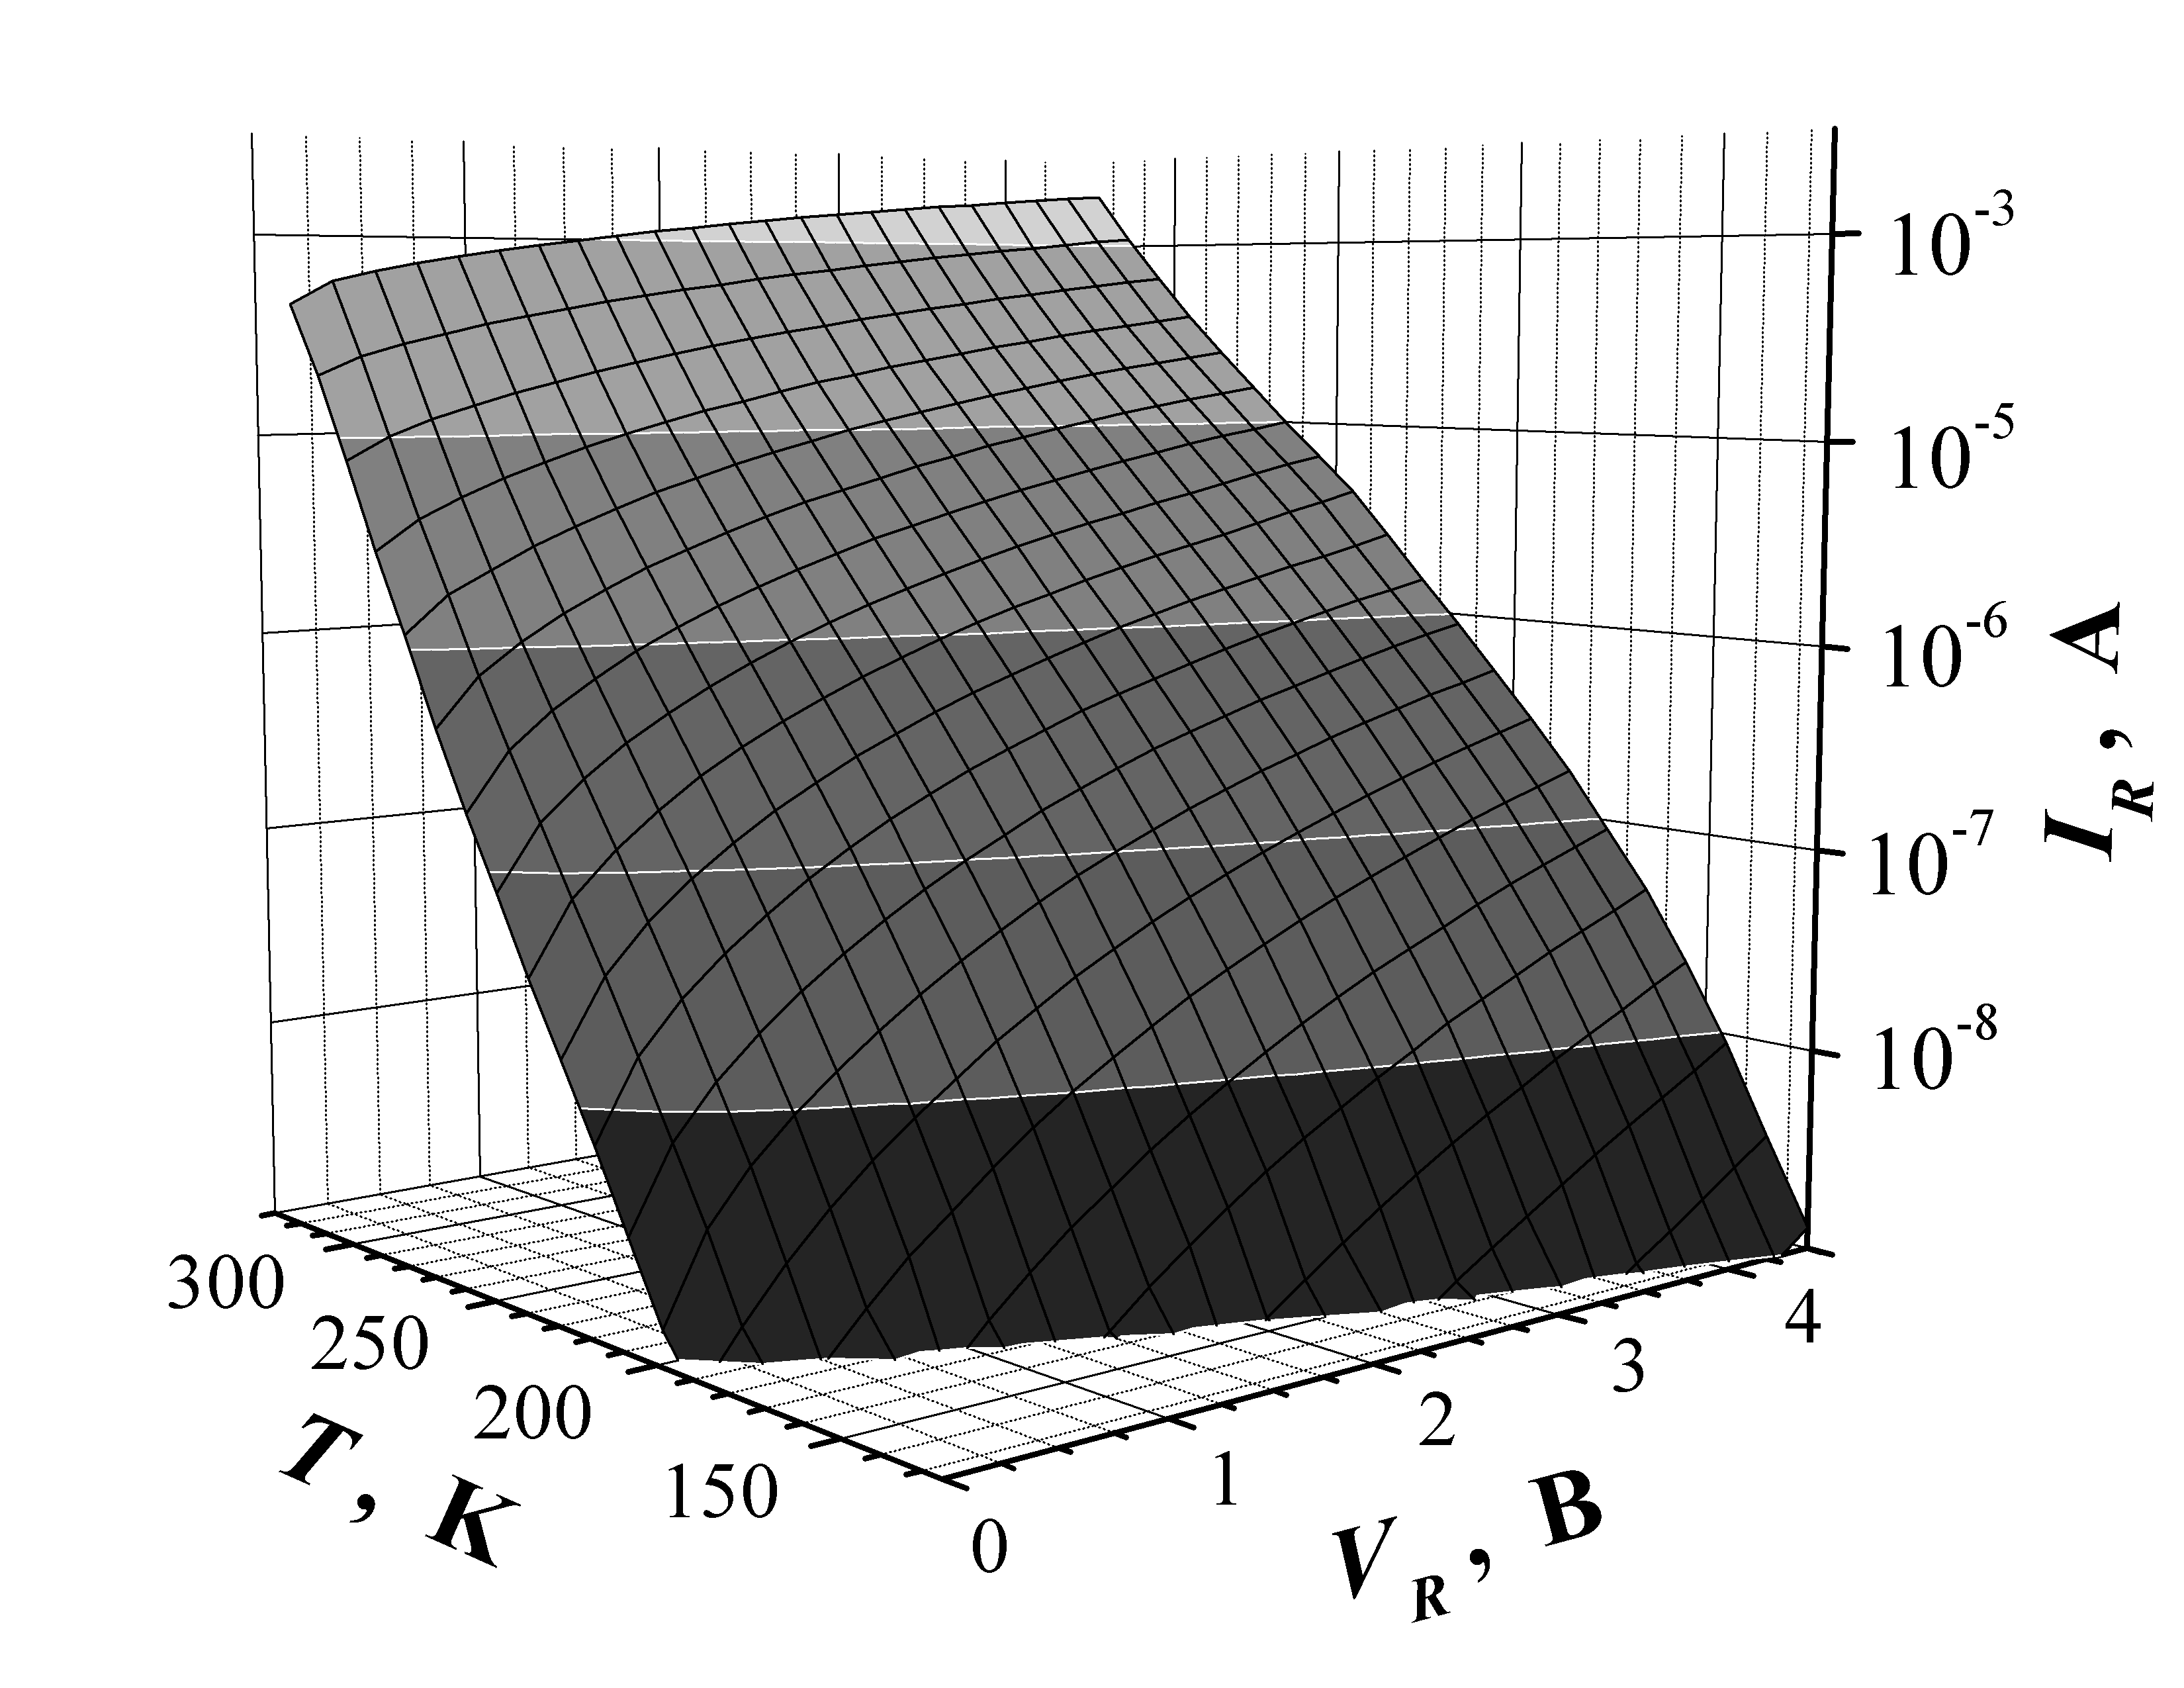
\includegraphics[width=0.75\textwidth]{figIVTr_SDB}
\caption{\label{figIVTr_SDB}
Залежності зворотного струму структур SSDB від напруги та температури.
}%
\end{figure}

\begin{figure}
\center
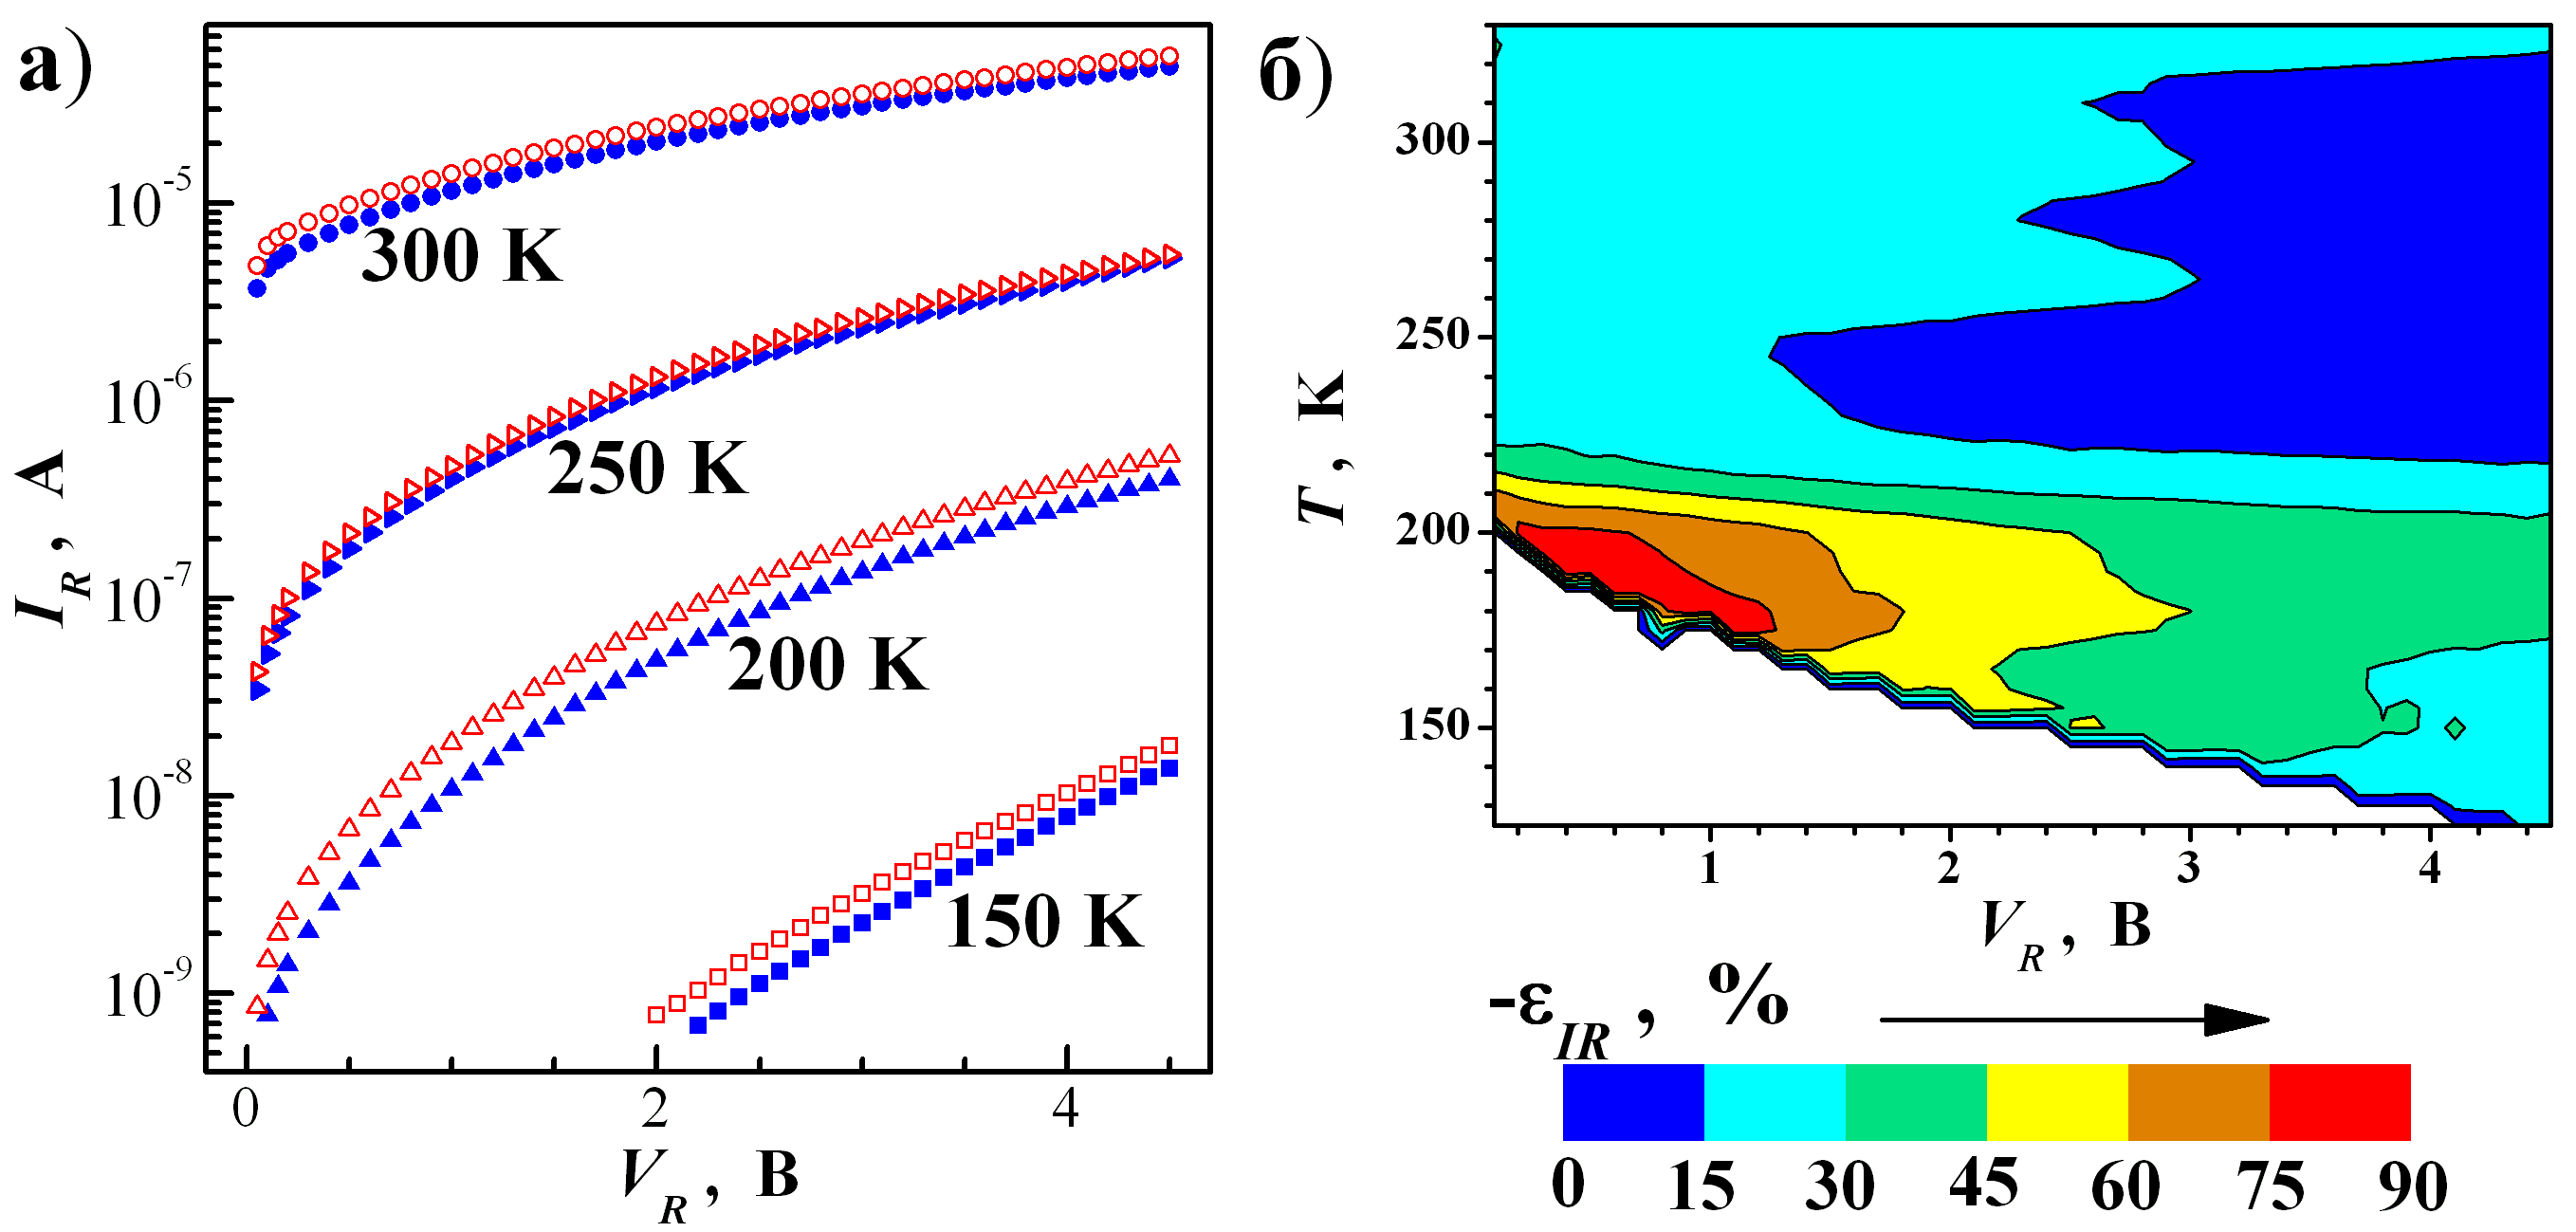
\includegraphics[width=0.95\textwidth]{figIVTrUS_SDB}
\caption{\label{figIVTrUS_SDB}
(a) Зворотні гілки ВАХ структур SSDB, виміряні за умов УЗН (порожні точки) та без нього (заповнені точки) при різних температурах.
(б) Залежності відносних АІ змін зворотного струму від зміщення та температури.
$f_\mathtt{US}=4,1$~MHz, $W_\mathtt{US}=0,65$~Вт/см$^2$.
}%
\end{figure}

\begin{figure}
\center
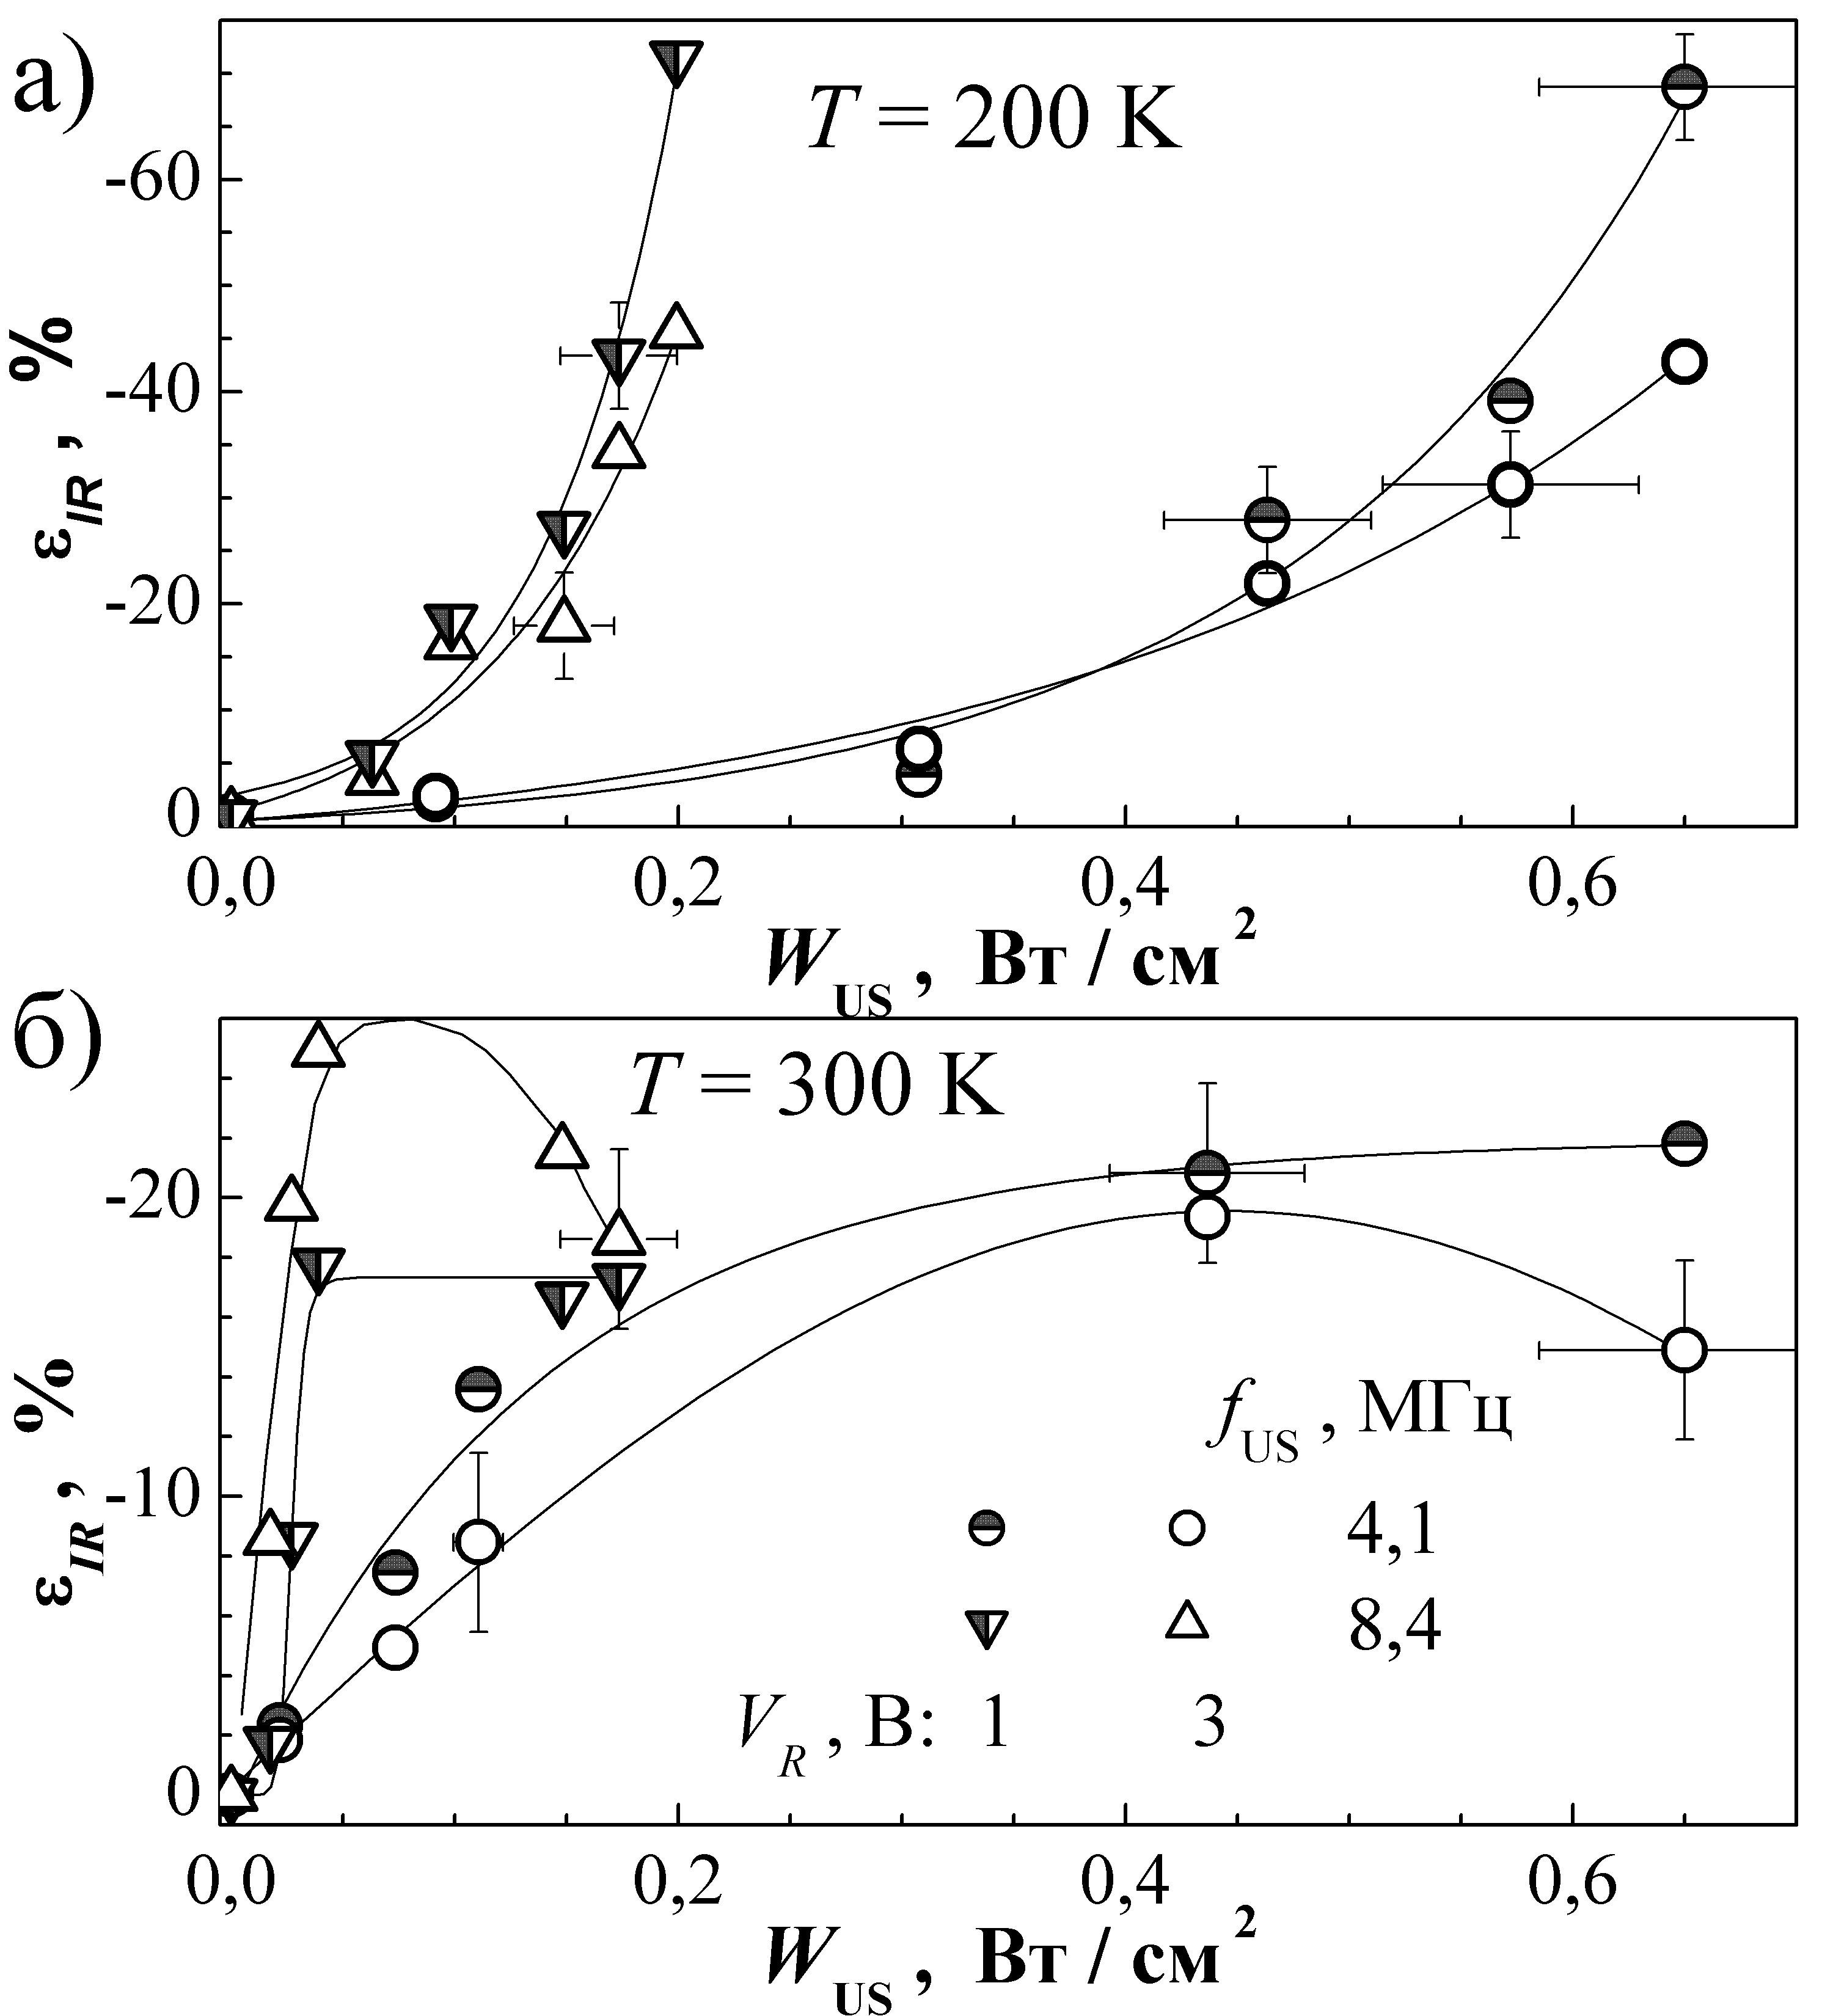
\includegraphics[width=0.6\textwidth]{figeIrWus_SDB}
\caption{\label{figeIrWus_SDB}
Залежності АІ відносних змін зворотного струму від інтенсивності УЗ.
$T$, K: 200 (a), 300 (б).
$f_\mathtt{US}$,~МГц: 4,1 (кола), 8,4 (трикутники).
Зміщення, В: 1 (порожні точки), 3 (заповнені точки).
Лінії наведено лише для зручності.
}%
\end{figure}

З рисунку~\ref{figIVTrUS_SDB},а видно, що УЗН викликає збільшення зворотного струму.
Зауважимо, що на цьому рисунку наведено лише незначна частина отриманих ВАХ ---
під час експерименту вимірювання проводилися кожні $4\div6$~К.
Виявлені АІ зміни зворотного струму оборотні і залежать як від температури, так і від величини зміщення ---
див. Рис.~\ref{figIVTrUS_SDB},б.
Нагадаємо, що від'ємні значення відносних змін зворотного струму $\varepsilon_{IR}$ відповідають
АІ зростанню цього параметру.
На рисунку представлено результати отримані під час УЗН U4SDB, проте вони є характерними і
для випадку використання інших частот.
Очевидно, що
\begin{enumerate}[label=\asbuk*),leftmargin=0em,itemindent=1.5em]
\item АІ збільшення зворотного струму може сягати декількох десятків відсотків;
\item при низьких температурах ефективність впливу УЗН зменшується як при зростанні зміщення, так і температури;
\item якщо температура перевищує 250~К то і польова, і температурна залежності $\varepsilon_{IR}$ стають слабкими.
\end{enumerate}

На Рис.~\ref{figeIrWus_SDB} показані зміни $\varepsilon_{IR}$ при збільшенні інтенсивності введеного УЗ.
Варто звернути увагу на дві особливості.
По--перше, характер АІ змін не залежить від $f_\mathtt{US}$,
проте при застосуванні більших частот УЗН спостерігається тенденція до збільшення величини зворотного струму
при тих самих значеннях $W_\mathtt{US}$.
По--друге, поведінка функції $\varepsilon_{IR}(W_\mathtt{US})$ суттєво залежить від температури:
насичення (або немонотонна залежність при великих зміщеннях) спостерігається у високотемпературному діапазоні
і різке збільшення акусто--керованих змін --- у низькотемпературному.





\subsection{Механізми струм втрат структур Mo$/n-n^+$--Si}

Цілком очевидно, що для з'ясування причин виявлених акусто--керованих ефектів важливо ідентифікувати
механізми перенесення заряду, які визначають характеристики досліджених структур.
Зазвичай подібна задача розв'язується шляхом аналізу температурних та польових залежностей струму.
На Рис.~\ref{figKT_SDB} представлені залежності зворотного струму від оберненої температури при різних напругах зміщення
у напівлогарифмічному масштабі.
На рисунку можна чітко виділити дві лінійні області, що свідчить про наявність двох механізмів
перенесення заряду.
Тобто зворотній струм складається з двох компонент $I_{1}$ та $I_2$:
\begin{equation}\label{eqIsum}
    I_R(T,V_R)=I_1(T,V_R)+I_2(T,V_R)\,,
\end{equation}
Як вже згадувалося, в літературі вказується на те, що в структурах МН поява струму може бути пов'язана з
різноманітними механізмами.
Проте, на нашу думку, одна з компонент пов'язана з ТЕ струмом, який є найбільш типовим для ДШ.
А отже, для $I_1$ може бути записаний наступний вираз

\begin{figure}
\center
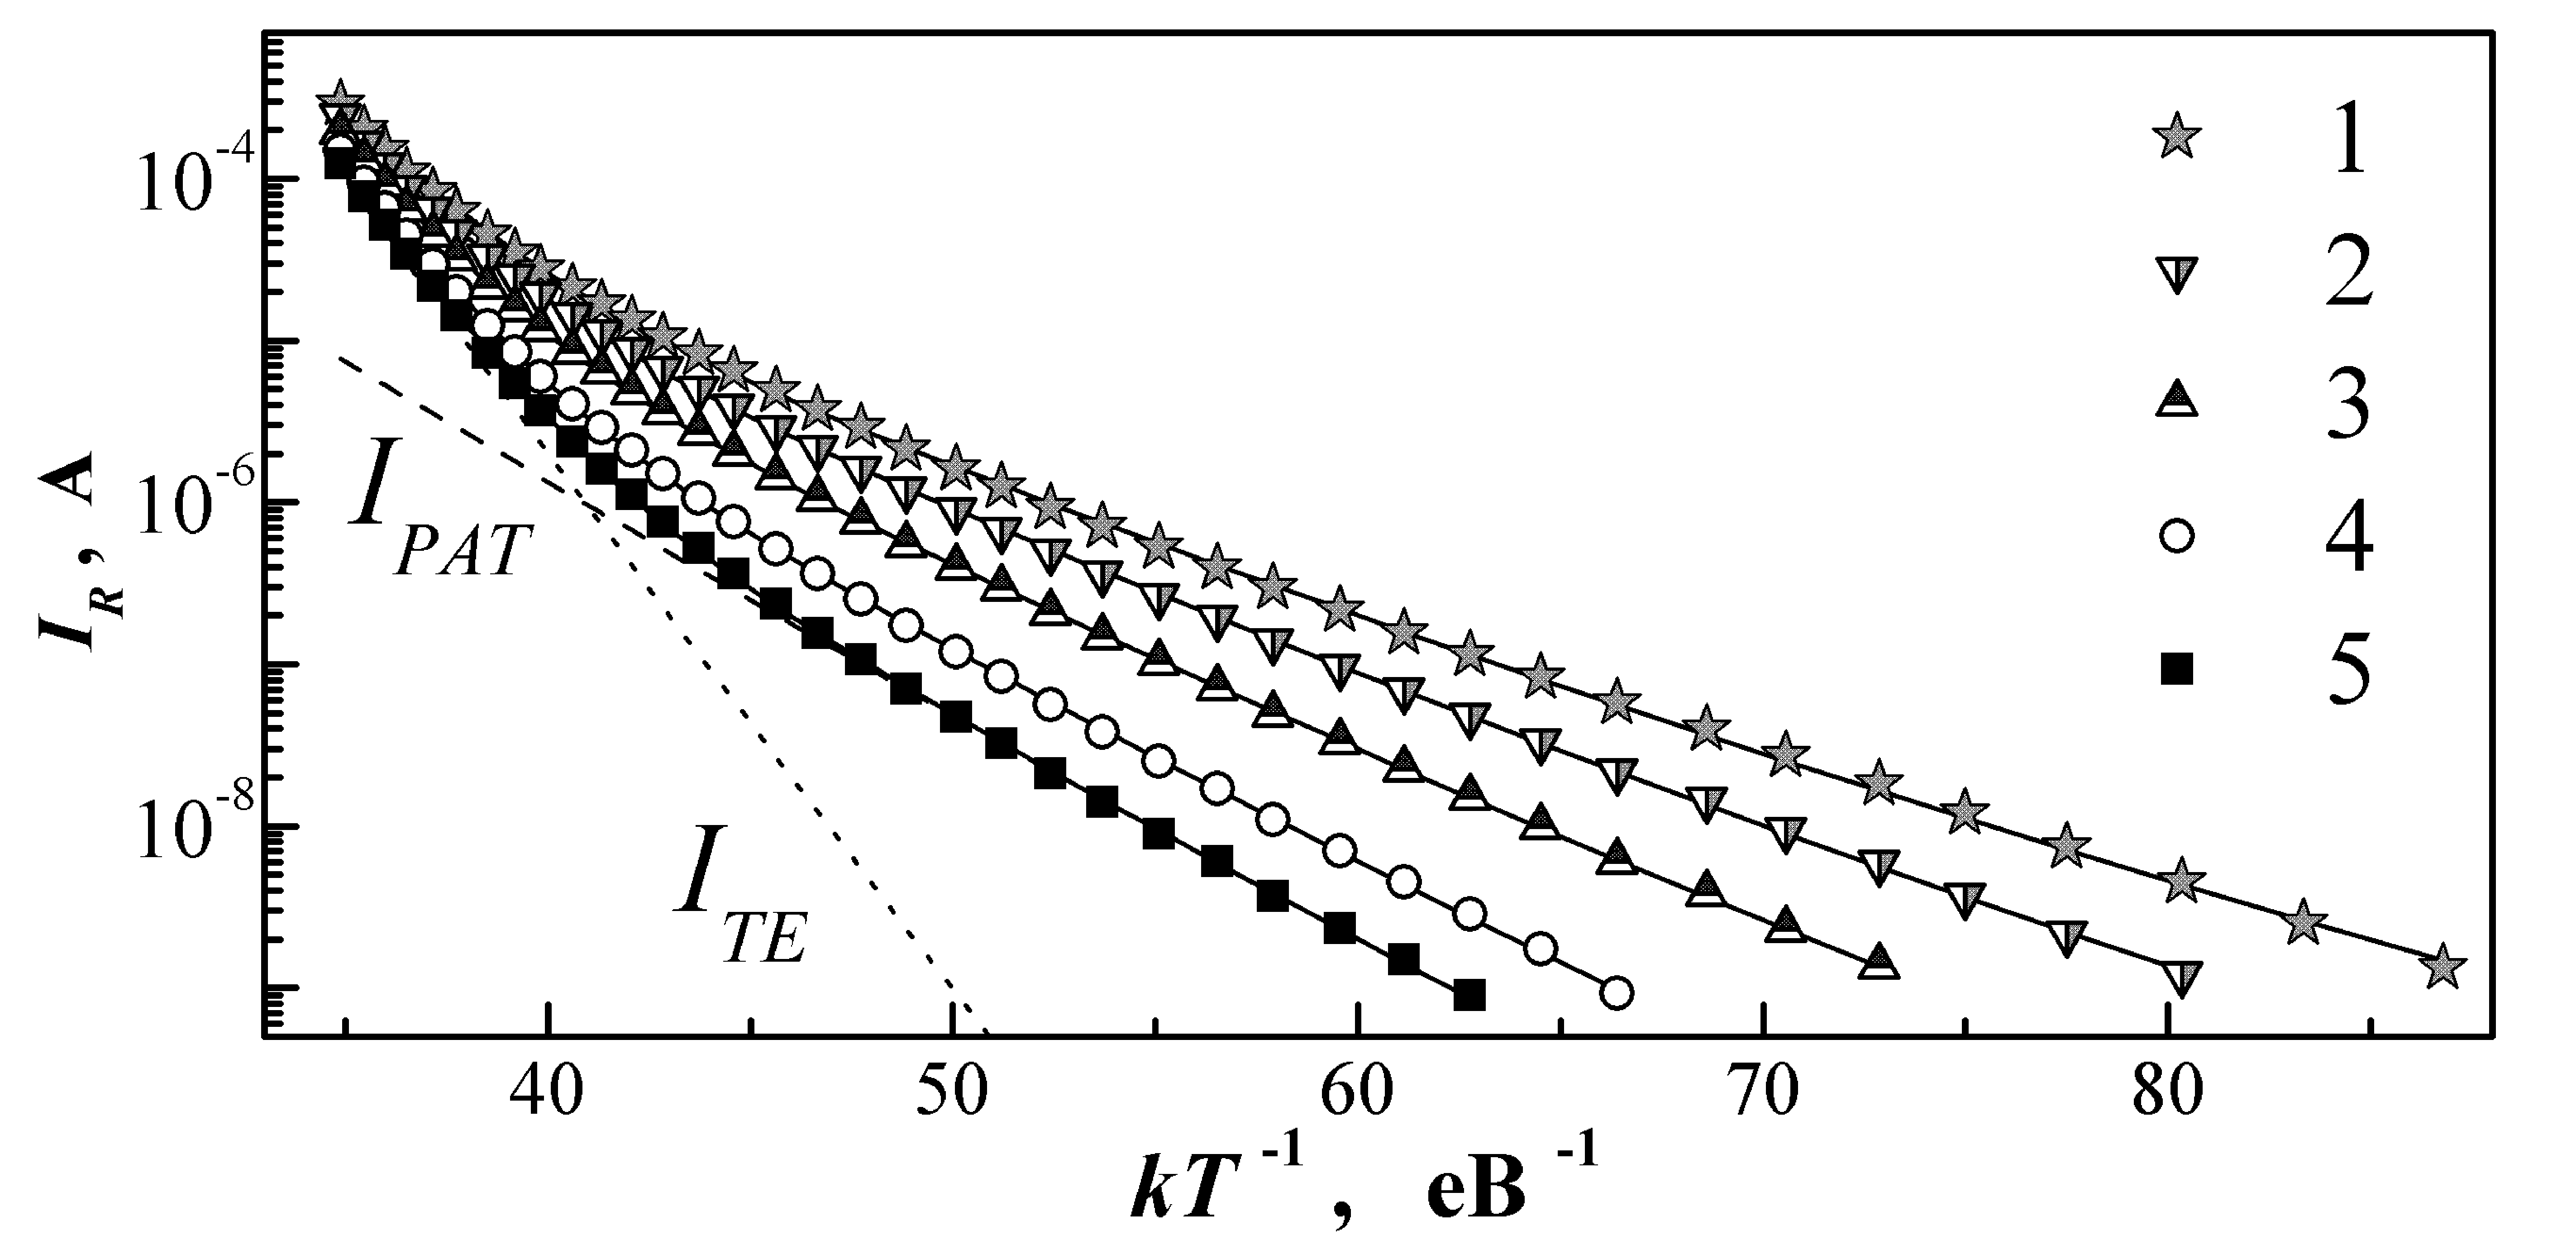
\includegraphics[width=0.9\textwidth]{figKT_SDB}
\caption{\label{figKT_SDB}
Залежність зворотного струму структур SSDB від оберненої температури,
виміряні при різних напругах зміщення.
Точки --- експеримент,
суцільні лінії --- відповідно до формули~(\ref{eqIgen}).
Пунктирна та штрихована лінії відображають ТЕ та РАТ компоненти струму, відповідно, для кривої 5.
$V_R$, В: 4 (1), 3 (2), 2 (3), 1 (4), 0.5 (5).
$W_\mathtt{US}=0$.
}%
\end{figure}

\begin{equation}\label{eqIte_SDB}
    I_1=I_0T^2\exp\left(-\frac{q\Phi_b}{kT}\right)\left[1-\exp\left(-\frac{V_R}{kT}\right)\right]\,,
\end{equation}
де $I_0$ --- певна константа,
причому для опису температурної залежності ВБШ $\Phi_b$ цілком застосовний вираз (\ref{eqFbT}).

При визначенні причин появи компоненти $I_2$ необхідно врахувати наступне.
SCLC провідність стає суттєвою за умови, що густина інжектованих вільних носіїв
набагато перевищує густину термічно генерованих \cite{Jafar}.
Тобто, SCLC є більш очікуваним при прямому зміщенні.
Модель VRHC передбачає появу низькотемпературного струму з малою енергією активації (декілька меВ) при
низьких значеннях напруженості електричного поля (омічний режим) \cite{Jafar}.
Ці умови також не відповідають нашому випадку, зокрема нахил кривих на Рис.~\ref{figKT_SDB} відповідає значно більшим значенням
активаційної енергії.
Таким чином цілком ймовірною причиною появи другої компоненти струму є процеси тунелювання, стимульованого фононами.
З літератури \cite{Pipinys1999,Pipinys2006} відомо, що цей механізм здатен пояснити залежності
зворотного струму в широкому температурному діапазоні і пов'язаний з тунелюванням
електронів з електронних пасток, розташованих біля інтерфейсного прошарку між металом на напівпровідником, в зону провідності останнього.
Згідно з \cite{Pipinys2006,Kiveris}, величина РАТ струму описується наступним чином:
\begin{eqnarray}
\label{eqIpat}
 I_{2}&=&\frac{q^2F_mAN_{ss}}{\sqrt{8m^*\epsilon_t}}\sqrt{\frac{\gamma_1-\gamma}{\gamma_1}}\exp
    \left\{-\frac{\sqrt{32m^*\epsilon_t^3}\left(\gamma_1-\gamma\right)^2}{3qF_m\hbar}
    [\gamma_1+\frac{1}{2}\gamma]\right\}, \\
    \gamma_1&=&(1+\gamma^2)^{1/2},\\
\label{eqIpat3}
    \gamma&=&\frac{a_\mathtt{e-ph}\hbar\omega_{ph}^2\sqrt{2m^*}}{qF_m\sqrt{\epsilon_t}}
    \left\{\frac{\exp\left(\frac{\hbar\omega_{ph}}{kT}\right)+1}{\exp\left(\frac{\hbar\omega_{ph}}{kT}\right)-1}\right\},
\end{eqnarray}
де
$N_{ss}$ --- густина заповнених рівнів поблизу інтерфейсу,
$\hbar\omega_{ph}$ --- енергія фонону,
$a_\mathtt{e-ph}$ --- константа електрон--фононної взаємодії,
глибина залягання рівня відносно зони провідності $\epsilon_t$,
напруженість електричного поля на границі розділу МН $F_m$ та інші величини зустрічалися раніше.

Формули (\ref{eqIsum})--(\ref{eqIpat3}) були використані для апроксимації експериментальних залежностей зворотного струму від температури.
Апроксимація здійснювалась з використанням методу диференційної еволюції.
При цьому величини $I_0$, $\epsilon_t$, $N_{ss}$ та ВБШ при нульовій температурі $\Phi_{b0}$ розглядалися як шукані параметри.
При розрахунках були використані значення $\hbar\omega_{ph}=16$~меВ, що відповідає повздовжнім акустичним фононам у Si \cite[с.~312]{ShalimovaBook}.,
та $a_\mathtt{e-ph}=6$, яке раніше застосовувалося  в роботі \cite{Pipinys1999} для найкращого узгодження синтезованих залежностей з експериментальними даними.
Результати, отримані для $I_0$, показано на Рис.~\ref{figI0V_SDB}.
З рисунку видно, що $I_0$ не залишається сталою, зменшуючись при збільшенні напруги зміщення.
З одного боку це суперечить класичній ТЕ теорії, а з другого --- свідчить
про необхідність враховувати наявність діелектричного прошарку між металом та напівпровідником.
Це означає, що
прикладена до структури напруга має бути представлена у вигляді



\begin{figure}
\center
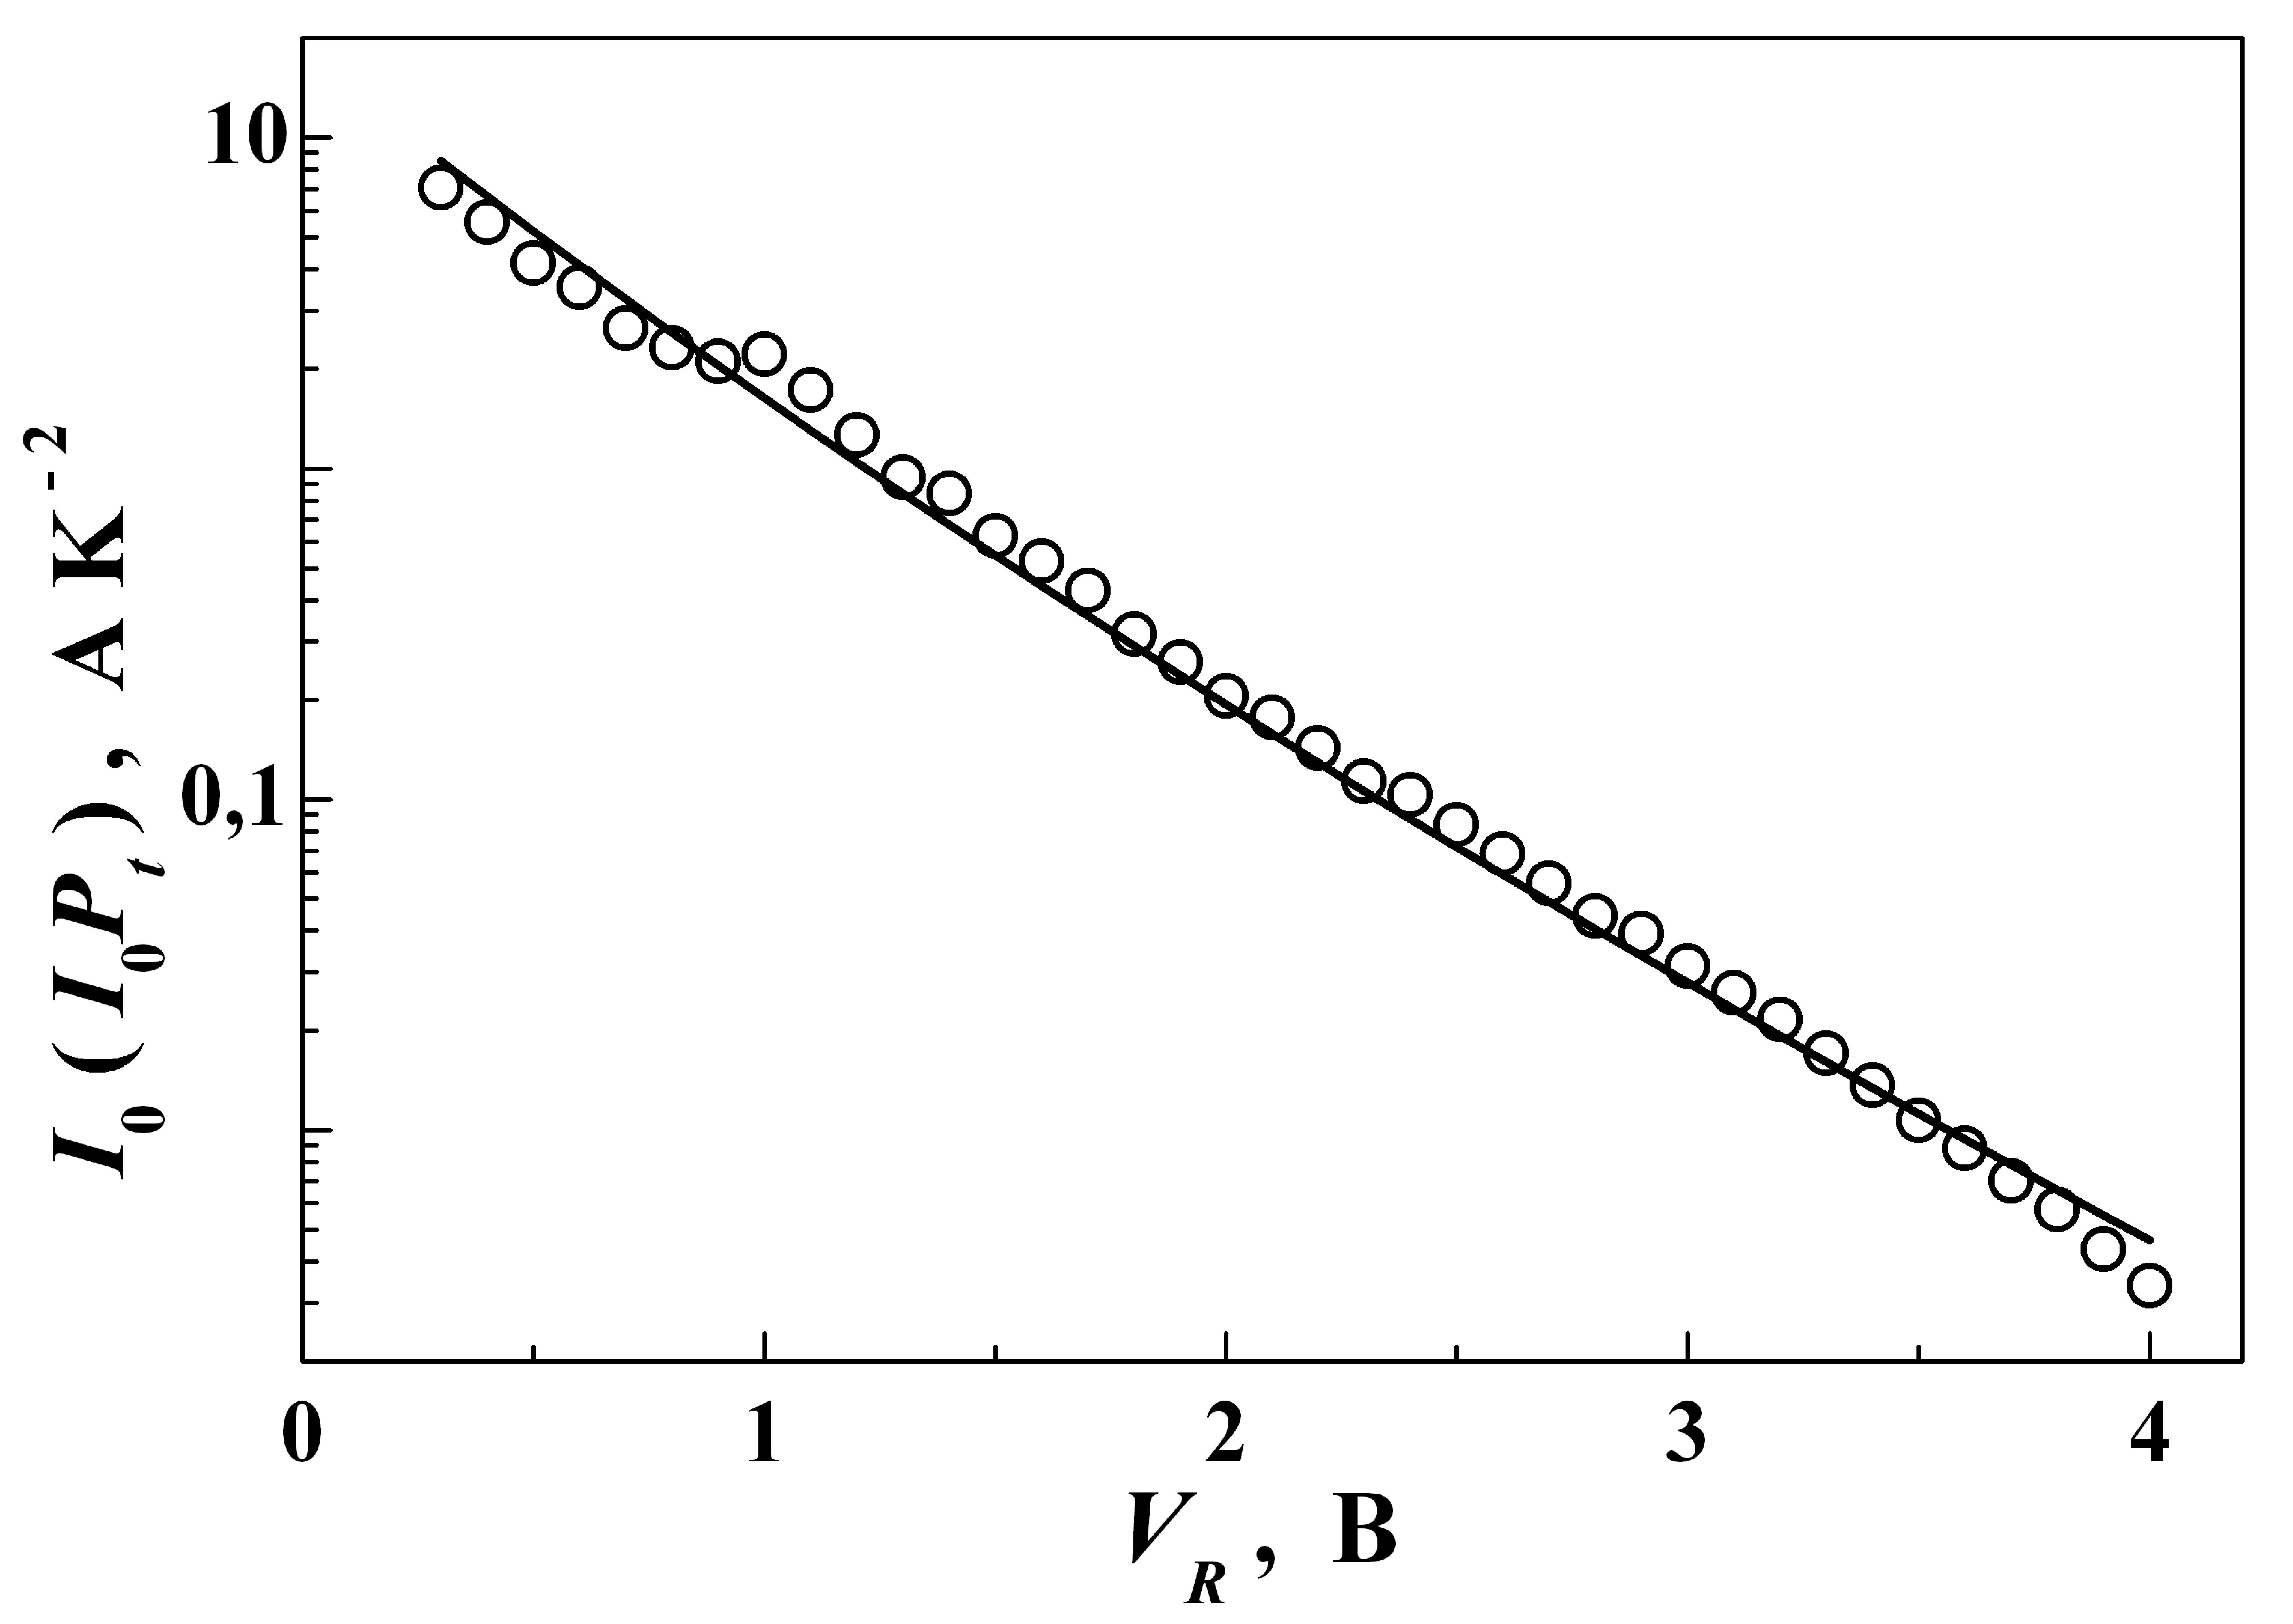
\includegraphics[width=0.6\textwidth]{figI0V_SDB}
\caption{\label{figI0V_SDB}
Залежність температуро--незалежного множника ТЕ струму від величини зворотної напруги.
Точки отримані з експериментальних даних,
лінія --- апроксимація з використанням формули~(\ref{eqPt}).
При розрахунках вважалося, що $V_i=0.5V_R$.
}%
\end{figure}


\begin{equation}\label{eqVR}
    V_R=V_i+V_s\,,
\end{equation}
де
$V_i$ та $V_s$ --- падіння напруги на ізолюючому прошарку та збідненому шару напівпровідника, відповідно.
Крім того, рівняння (\ref{eqIsum}) має бути замінено на
 by
\begin{equation}\label{eqIsum2}
    I_R(T,V_R)=P_t(V_i)\times[I_1(T,V_s)+I_2(T,V_s)]\,,
\end{equation}
де
$P_t$ --- ймовірність переміщення (тунелювання) заряду через ізолюючий прошарок.
З врахуванням цих змін необхідно зазначити, що Рис.~\ref{figI0V_SDB} відображає залежність не $I_0$,
а добутку $P_tI_0$.

У випадку, якщо з діелектричним прошарком пов'язаний трапецоїдальний потенційний бар'єр,
то ймовірність квантово--механічного тунелювання описується виразом
\begin{equation}\label{eqPt}
    P_t=\exp\left\{-\frac{4\sqrt{2m_i^*q}}{3\hbar V_i}\left[(U_0+V_i)^{\,3/2}-U_0^{\,3/2}\right]\delta\right\}\,,
\end{equation}
де
$U_0$ --- висота бар'єру на границі напівпровідник/ізолятор при нульовому зміщенні,
$m_i^*$ --- ефективна маса електрону в ізоляторі,
$\delta$ --- товщина діелектричного прошарку.
Використовуючи значення $m_i^*=0,5m_0$ (що відповідає SiO$_2$)
та $V_i=0,5V_R$, була проведена апроксимація даних на Рис.~\ref{figI0V_SDB} з використанням формули
(\ref{eqPt}).
Результати показані на рисунку суцільною лінією.
Отримані значення параметрів $U_0=1$~В та $\delta=2,8$~нм є цілком реальними: наприклад,
в літературі повідомляється, що товщина шару окису може складати від $0,2\div1$~нм на поверхні кремнієвих пластин \cite{Saito}
до 10,2~нм на інтерфейсі ДШ \cite{SHIWAKOTI2018}.
Це підтверджує застосовність використаних припущень.

Таким чином, узагальнений вираз для зворотного струму набуває вигляд
\begin{eqnarray}
\label{eqIgen}
 I_R&=&I_{TE}+I_{P\!AT}=P_tI_0\,T^2\exp\left(-\frac{q\Phi_b}{kT}\right)\left[1-\exp\left(-\frac{V_s}{kT}\right)\right]+\\
 &&+\frac{P_tq^2F_mAN_{ss}}{\sqrt{8m^*\epsilon_t}}\left(1-\frac{\gamma}{\gamma_1}\right)^{1/2}\exp
    \left\{-\frac{4\sqrt{2m^*}\,\epsilon_t^{3/2}\left(\gamma_1-\gamma\right)^2}{3qF_m\hbar}
    [\gamma_1+\frac{1}{2}\gamma]\right\}\nonumber,
\end{eqnarray}
де
$I_{TE}$ та $I_{P\!AT}$ --- ТЕ та РАТ компоненти струму, відповідно,
причому для обчислення $F_m$ у виразі (\ref{eqFm}) замість $V_R$ має бути використано $V_s$.
Формула (\ref{eqIgen}) була використана для апроксимації експериментальних даних.
При цьому вважалося, що $V_s=0.5V_R$.
Результати апроксимації представлені лініями на Рис.~\ref{figKT_SDB}.
Для всього діапазону напруг середньоквадратичне відхилення апроксимуючих кривих від експериментальних даних не перевищувало 0,7\%.
Польові залежності визначених параметрів показані на Рис.~\ref{figField_SDB}, криві 1.
Для розрахунку $N_{ss}$ були використані значення $P_t$, отримані з Рис.~\ref{figI0V_SDB}.

\begin{figure}
\center
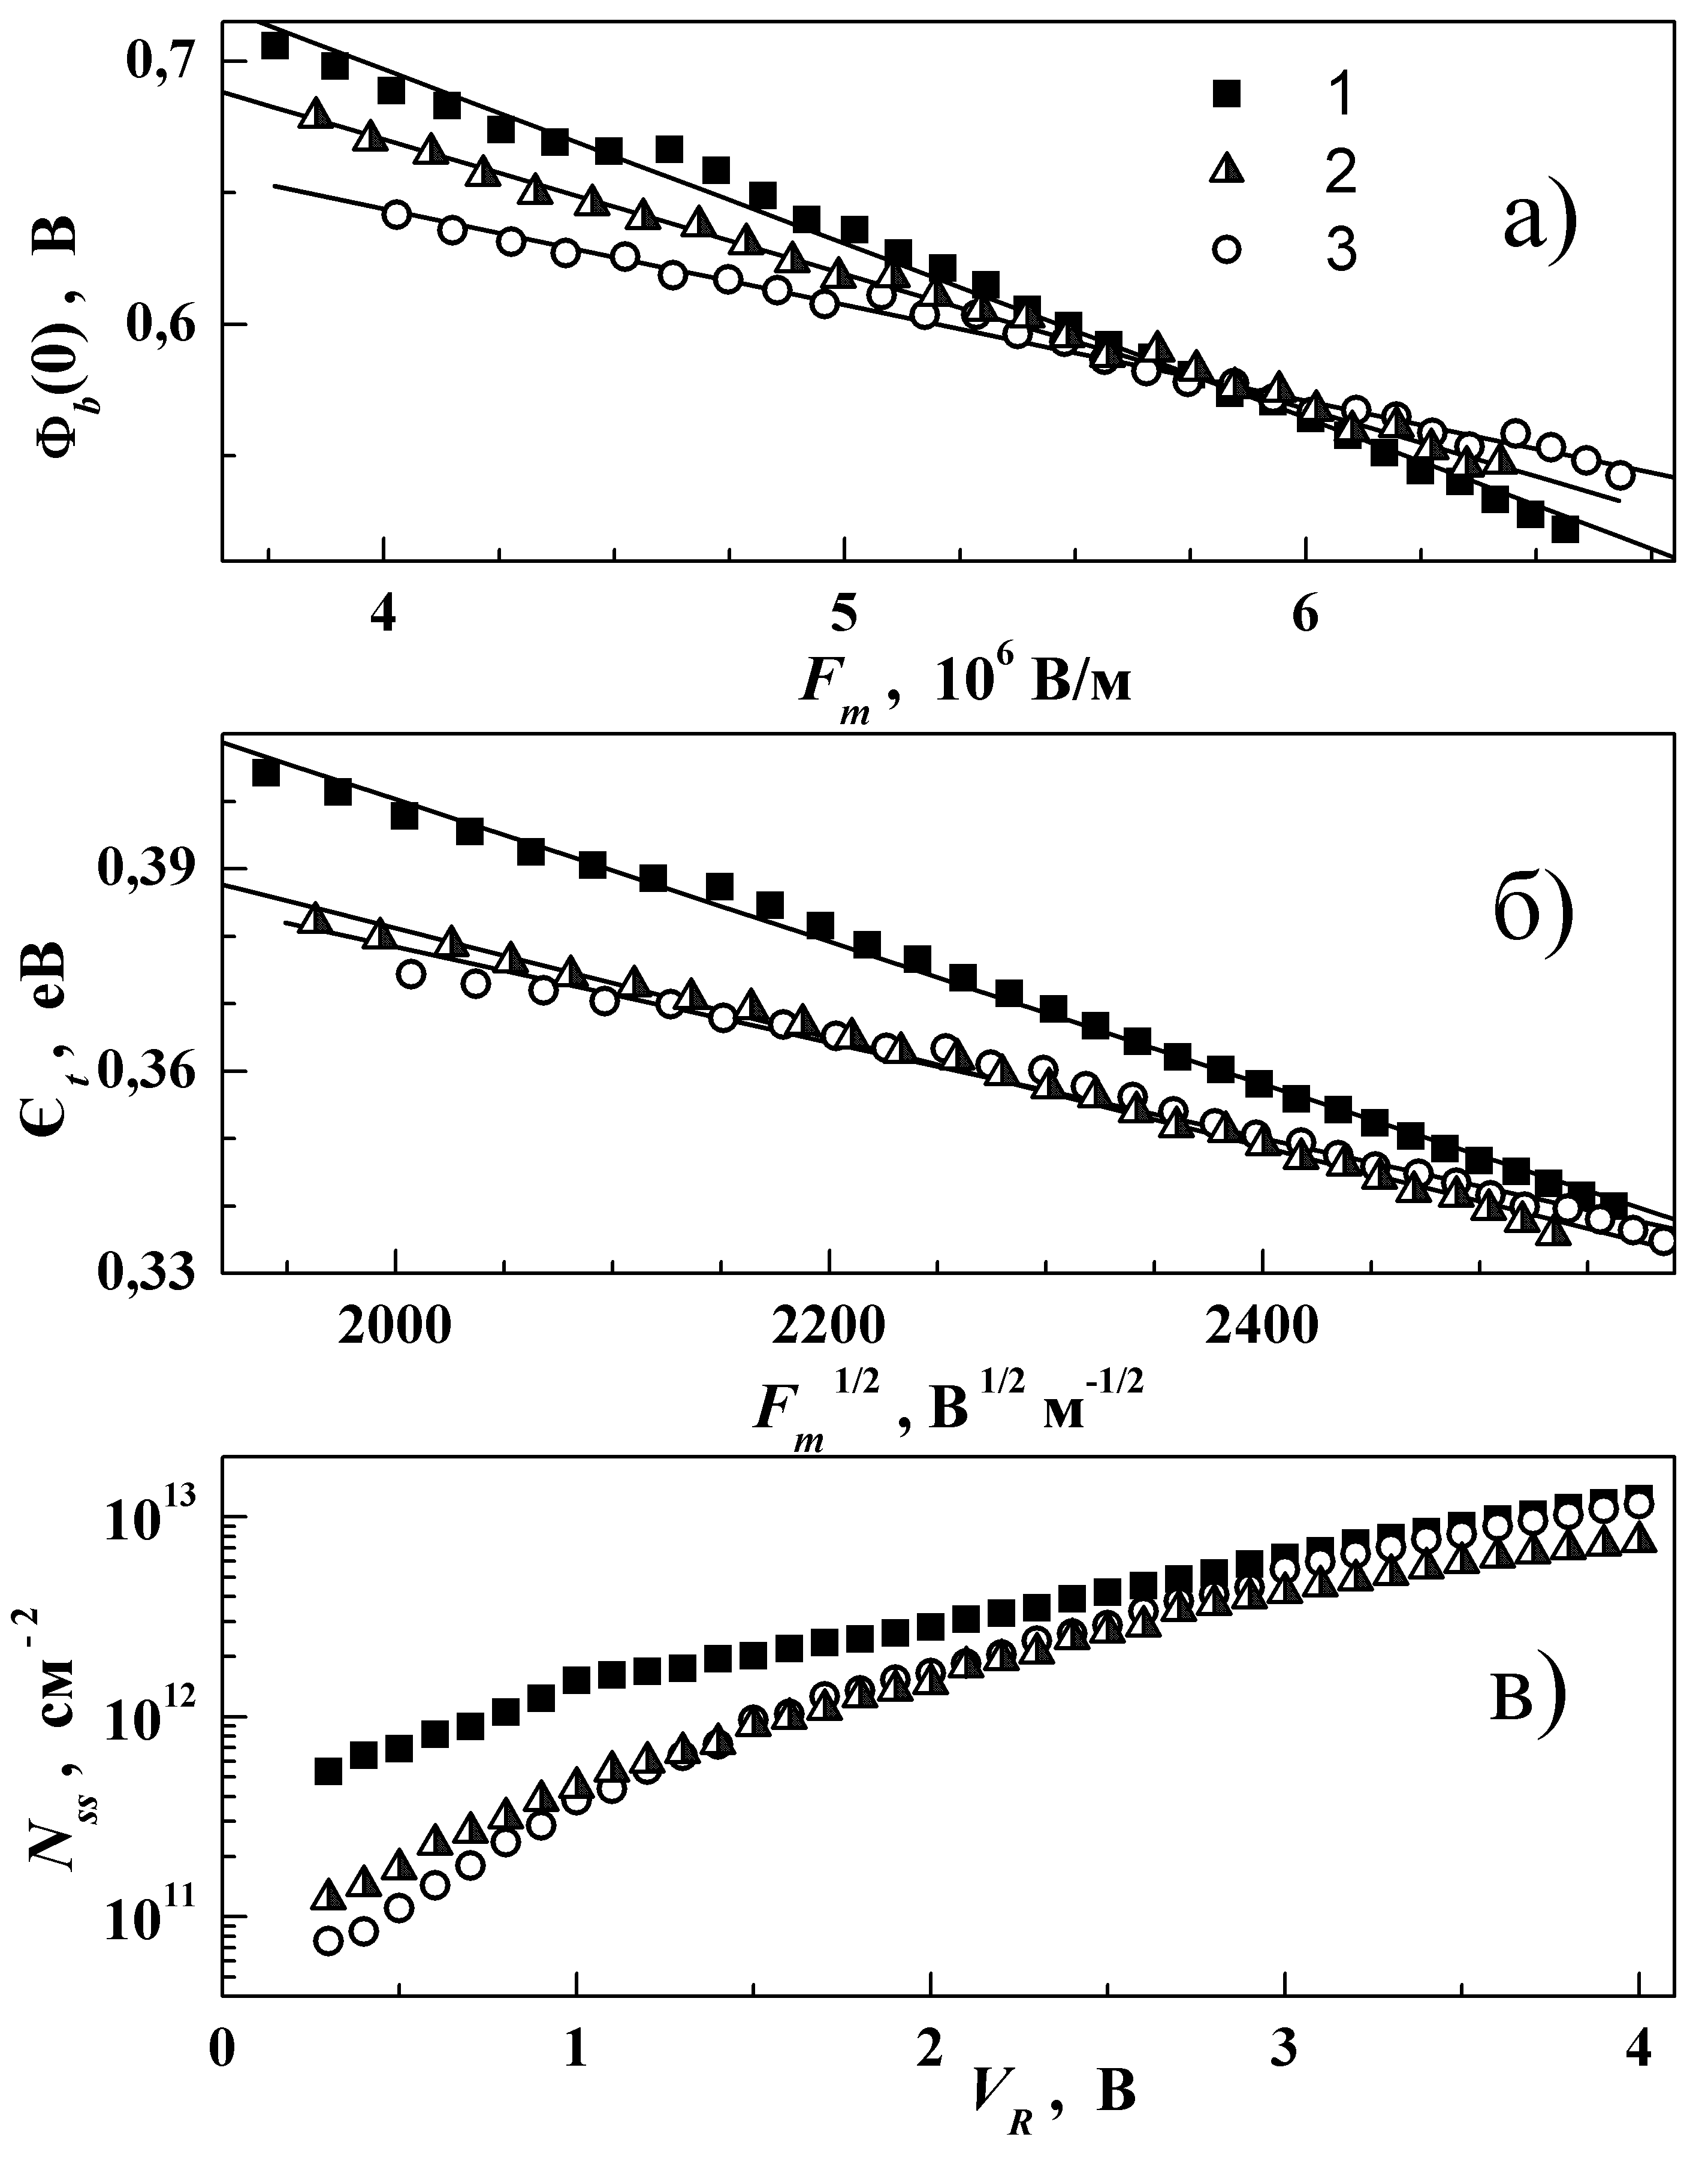
\includegraphics[width=0.6\textwidth]{figField_SDB}
\caption{\label{figField_SDB}
Польові залежності ВБШ (а), енергії активації пастки (б) та густини інтерфейсних станів (в) для структур SSDB за умов УЗН (2 та 3) та без нього (1).
$W_\mathtt{US}$,~Вт/см$^2$: 0 (1), 0,17 (2), 0,65 (3).
$f_\mathtt{US}$,~МГц: 8,4 (2), 4,1 (3).
}%
\end{figure}

Виявлено (див. Рис.~\ref{figField_SDB},а), що зниження ВБШ пропорційне $F_m$:
\begin{equation}\label{eqFbE}
    \Phi_{b}(0)=\Phi_{b0}(0)-\alpha_{F} F_m\,.
\end{equation}
Відомо \cite{Tung:MSE,Rhoderick1988,Em:Parker},
що подібна залежність спостерігається у випадку, коли зниження висоти бар'єру переважно визначається інтерфейсними рівнями.
При цьому  $\alpha_{F}$ визначає положення максимуму потенціалу, що є результатом суперпозиції поля Шотки та поля поверхневих станів \cite{Em:Parker}.

Отримане значення $\epsilon_t$ ($0.35\div0.40$~еВ) приблизно втричі менше ширини забороненої зони кремнію.
Подібні співвідношення і раніше були виявлені при дослідженні РАТ--струму:
наприклад, енергія активації електронів з пастки дорівнювала $0.50$~еВ для GaAs \cite{Pipinys1999} та $0.90$~еВ для GaN \cite{Pipinys2006}.
Як видно з наведених даних (Рис.~\ref{figField_SDB},б),
енергія активації зменшується при зростанні напруженості електричного поля,
причому зниження пропорційне квадратному кореню з $F_m$:
\begin{equation}\label{eqEtE}
    \epsilon_t=\epsilon_{t0}-\beta_F F_m^{1/2}\,,
\end{equation}
де
$\epsilon_{t0}$ --- енергія зв'язку електрона на пастці за відсутності поля.
Подібний механізм польової емісії відомий в літературі як ефект Пула--Френкеля.
Величина $\epsilon_{t0}=0.61$~еВ є близькою до рівня іонізації дефектів, пов'язаних з вакансіями, у об'ємному кремнії \cite{Seebauer,VI:Luc}.
Цілком ймовірно, що пастки, які беруть участь у тунелюванні, пов'язані саме з дефектами подібного типу.
Очікується \cite{PF:Mitrofanov,PF:ZhdanovaR}, що для параметру $\beta_F$ справедливе наступне співвідношення
\begin{equation}\label{eqBetta}
    \beta_F=\sqrt{\frac{Zq^3}{\pi\varepsilon_0\varepsilon_s}}\,,
\end{equation}
де
$Z$ --- заряд центру.
Для однократно зарядженої пастки в Si теоретичне значення параметру $\beta_{PF}$, обчислене використовуючи
рівняння (\ref{eqBetta}), дорівнює $2,2\cdot10^{-5}$~еВ(м/В)$^{1/2}$.
В нашому випадку отримане значення ($10,5\cdot10^{-5}$~еВ(м/В)$^{1/2}$) відрізняється від $\beta_{PF}$.
Подібні відхилення також описані в літературі.
Так, з одного боку, вираз (\ref{eqBetta}) справедливий в одномірному наближенні та величини  $\beta_F<\beta_{PF}$ спостерігалися експериментально \cite{PF:Mitrofanov,PF:ZhdanovaR}.
З іншого боку, згідно з \cite{PF:ZhdanovaR}, електрони можуть бути захоплені на пастки, розташовані в кластері позитивно заряджених іонів, утворення яких має флуктуаційний характер.
Це викликає збільшення як ефективної кратності виродження (до 10--30 \cite{PF:ZhdanovaR}), так і величини $\beta_F$.
Амплітуда збільшення залежить від розміру кластера.
Саме з цим ефектом, на нашу думку, і пов'язана відмінність отриманого значення від $\beta_{PF}$.
Всі отримані параметри зведено до Таблиці~\ref{tabSDBParZv} (перший рядок).




\begin{table}
\caption{Параметри, визначені для структур Mo$/n-n^+$--Si зі зворотних гілок ВАХ за умов УЗН та без нього}
\label{tabSDBParZv}
\centering
\begin{tabular}{|c|c|c|c|c|c|}
\hline
$W_\mathtt{US}$, &$f_\mathtt{US}$,&$\Phi_{b0}(0)$,&$\alpha_F$,&$\epsilon_{t0}$,&$\beta_F$,\\
Вт/см$^2$&МГц&мВ&нм&меВ&$10^{-5}$~еВ$\cdot$м$^{1/2}\cdot$В$^{-1/2}$\\\hline
0&---&$960\pm10$&$66\pm7$&$610\pm10$&$10,5\pm0,3$\\\hline
0,17&8,4&$870\pm10$&$51\pm5$&$540\pm10$&$\;\:8,1\pm0,5$\\\hline
0,65&4,1&$790\pm10$&$36\pm7$&$520\pm10$&$\;\:7,1\pm0,5$\\\hline
\end{tabular}
\end{table}



\subsection{Ефект впливу ультразвуку на характеристики перенесення заряду}

Описана вище процедура була також використана для апроксимації залежностей зворотного струму, виміряних за умов УЗН.
Отримані при використанні двох режимів УЗН результати зведені на Рис.~\ref{figField_SDB} (криві 2 та 3) та в Таблиці~\ref{tabSDBParZv} (другий та третій рядки).
Виявлено, що УЗН впливає як на ТЕ, так і РАТ компоненти струму.
Зокрема, спостерігається АІ зменшення енергії активації носіїв, захоплених на пастки --- див. Рис.~\ref{figField_SDB},б.
Подібний ефект може бути зв'язаний зі зміною заселеності коливальних рівнів дефекту \cite{Pavlovich} або зі зміщенням домішкових
атомів відносно їх оточення \cite{Korotchenkov1995}.
Згідно з розрахунками, проведеними в роботі \cite{Pavlovich}, ефективність АДВ має збільшуватись при зростанні частоти УЗ;
ці очікування співпадають з результатами експерименту.

В свою чергу, якщо електрон потребує меншої енергії для звільнення з пастки,
то можна очікувати, що УЗН має викликати зменшення густини заповнених станів.
Саме така тенденція і спостерігається в нашому випадку ---- див. Рис.~\ref{figField_SDB},в.
Зауважимо, що вплив УЗ на пастки зменшується зі зростанням напруженості електричного поля.

Згідно з результатами, представленими в роботі \cite{Em:Parker},
величина $\alpha_F$ має зростати при збільшенні концентрації заряджених поверхневих станів та
глибини проникнення поля, пов'язаного  з ними.
Таким чином, зменшення рівноважної кількості захоплених на поверхні електронів може бути причиною виявленого акусто--індукованого
зменшення параметра $\alpha_F$.

На нашу думку, АІ зменшення коефіцієнту $\beta_F$ відбувається внаслідок зміни розміру дефектного кластера і викликаної цим
модифікації ефективної кратності заряду.
Можливою причиною цього процесу є локальне підвищення кластеру дефектів в акустичному полі.
Цей ефект описано в роботі \cite{MirzadeJAP2011}.

Отримані дані показують, що ВБШ зменшується під дією УЗН.
Ці результати співпадають з отриманими з аналізу прямих гілок ВАХ і детально описаними в попередніх параграфах.

Для більш чіткого розуміння польових та температурних залежностей АІ змін зворотного струму $\varepsilon_{IR}$ (Рис.~\ref{figIVTrUS_SDB},б)
розглянемо відносний внесок РАТ компоненти зворотного струму
Нагадаємо, що від'ємні значення відносних змін зворотного струму
$\nu_\mathrm{PAT}=I_{P\!AT}/(I_{P\!AT}+I_{TE})$.
На Рис.~\ref{figPartial_SDB},a наведено залежності $\nu_\mathrm{PAT}$ від напруги та температури для ненавантаженого зразка,
а на Рис.~\ref{figPartial_SDB},б --- зміни $\nu_\mathrm{PAT}$ під дією УЗ.


\begin{figure}
\center
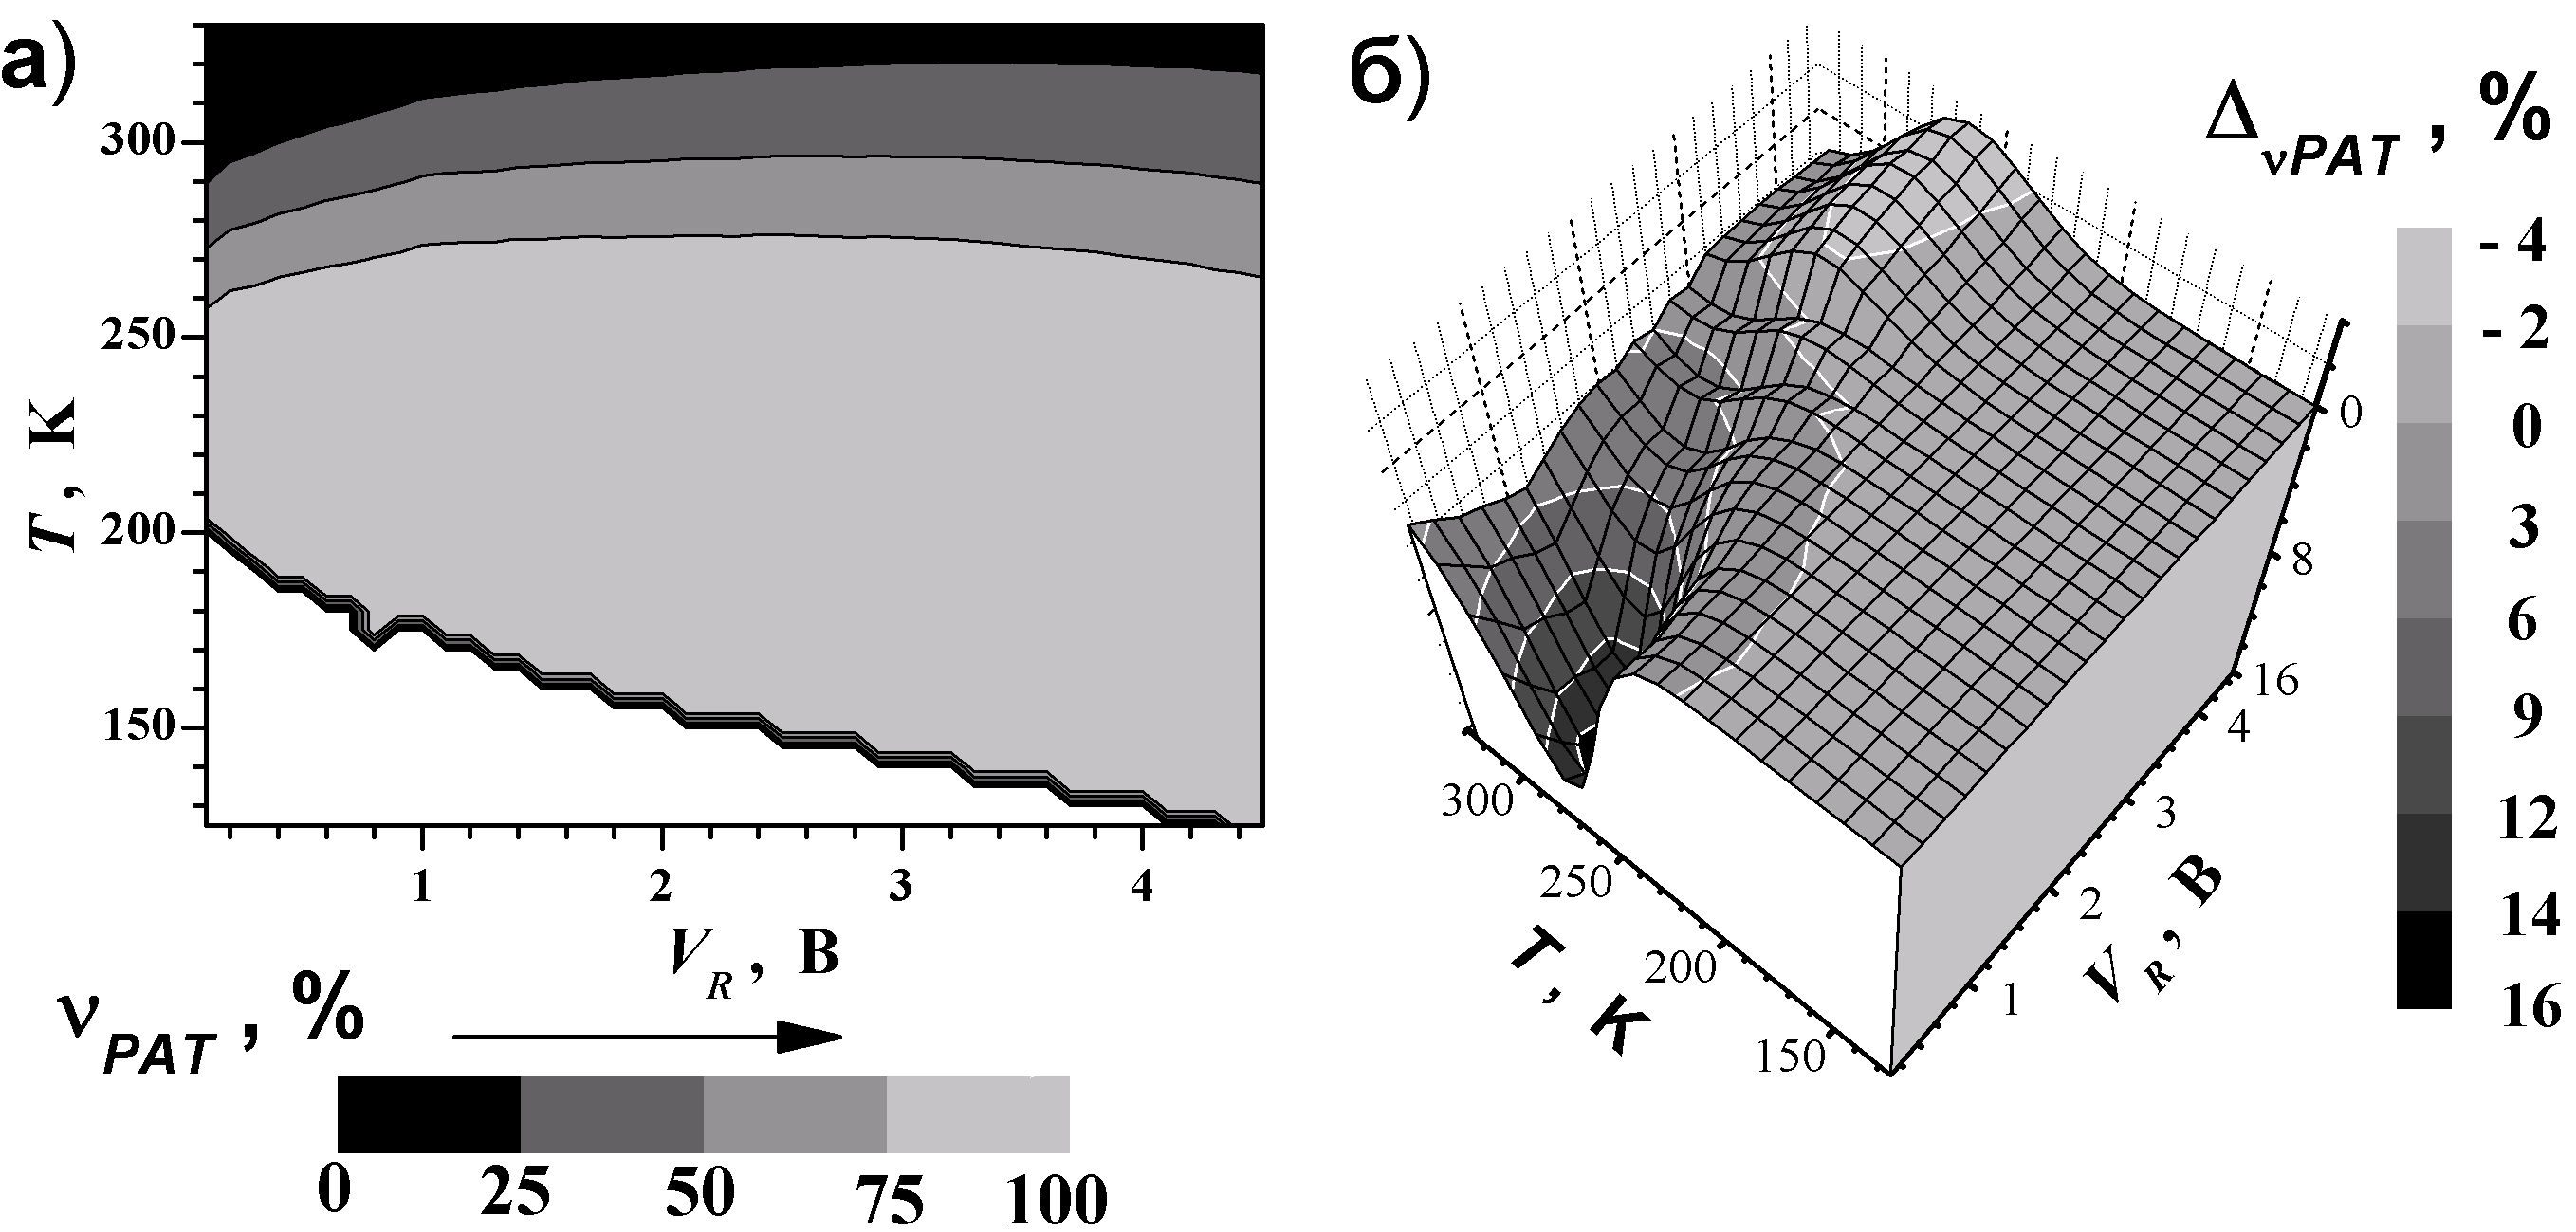
\includegraphics[width=0.95\textwidth]{figPartial_SDB}
\caption{\label{figPartial_SDB}
Залежності парціального внеску РАТ компоненти зворотного струму від напруги та температури (а)
та його АІ зміни при дії УЗ з $f_\mathtt{US}=4,1$~МГц, $W_\mathtt{US}=0,65$~Вт/см$^2$ (б).
}%
\end{figure}

Як видно з наведених даних, РАТ компонента є переважаючою при низьких температурах, тоді як термоемісійна складова стає превалюючою при $T>260$~K.
Крім того, варто взяти до уваги, що
а)~зменшення $\epsilon_{t0}$ та $\beta_F$ (так само як і $\Phi_{b0}(0)$ та $\alpha_F$) викликають протилежні зміни величини зворотного струму;
б)~ВБШ сильніше залежить від напруженості електричного поля, ніж енергія активації з пасткового рівня
(зміни $\Phi_{b}(0)$ та $\epsilon_t$ складають 25\% та 15\%, відповідно -- див. Рис.~\ref{figField_SDB}),
проте РАТ струм явно залежить від $F_m$ -- див. формулу~(\ref{eqIpat}).



\begin{figure}
\center
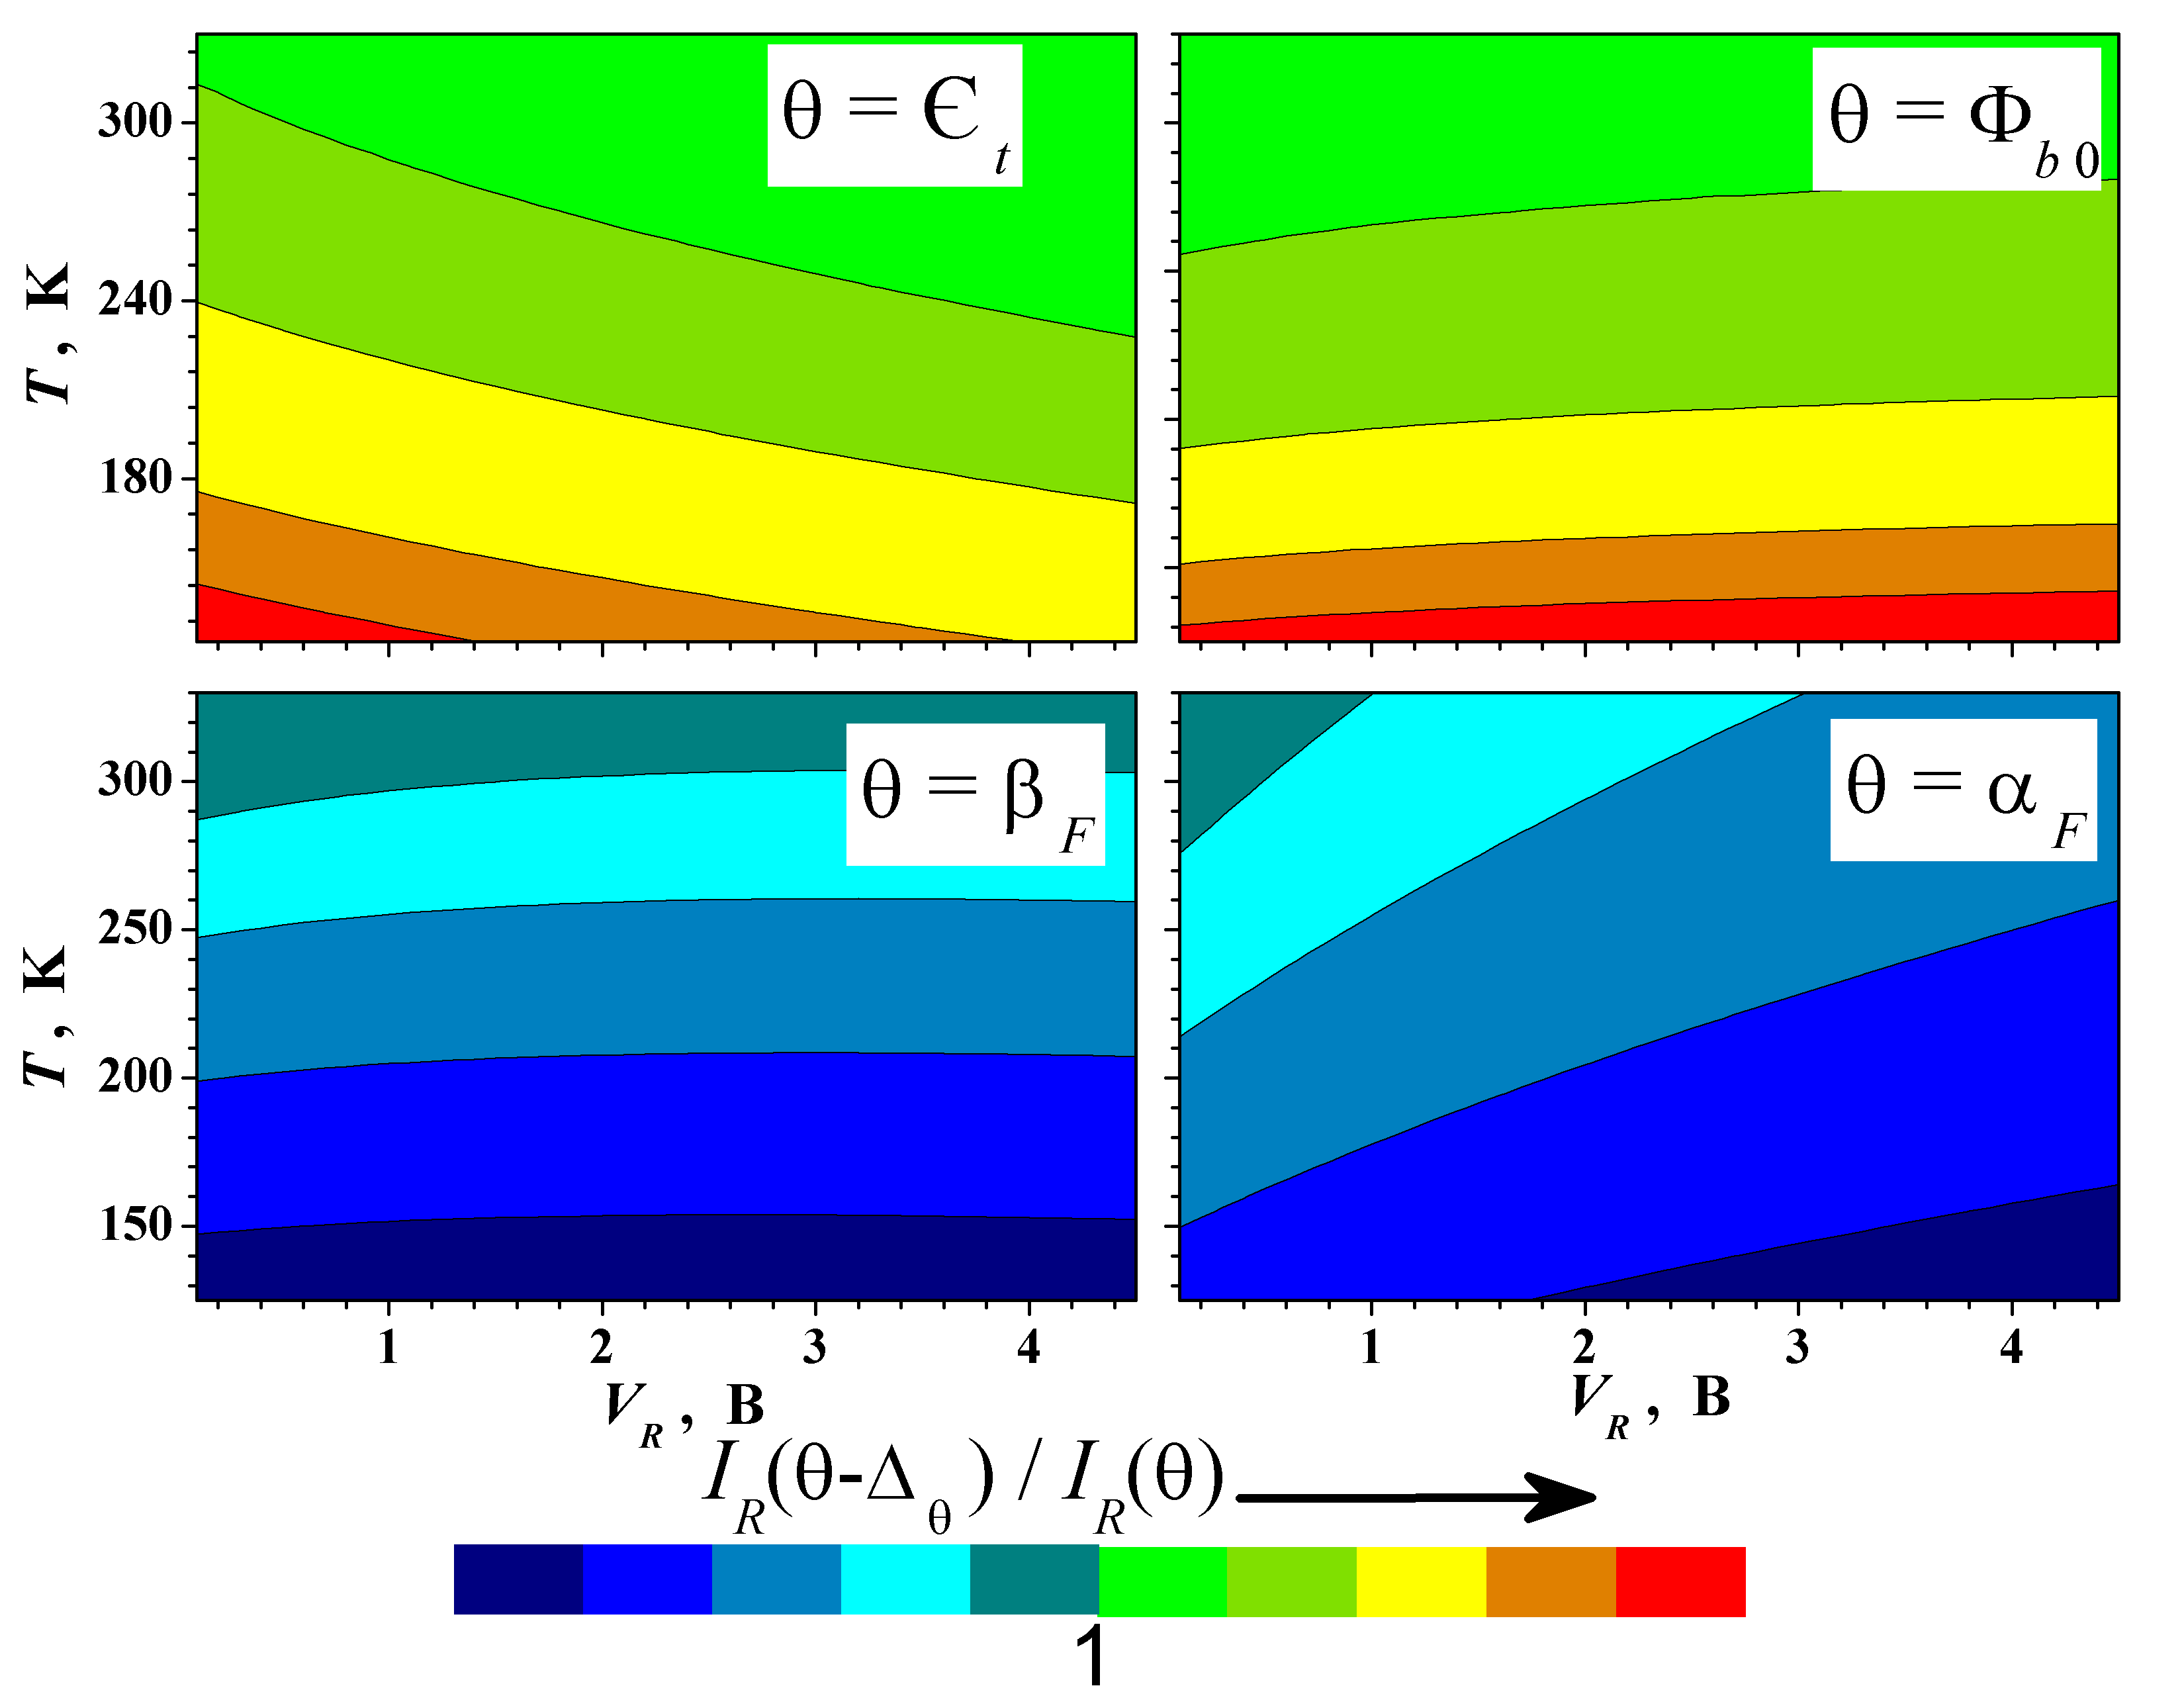
\includegraphics[width=0.8\textwidth]{figRozrah_SDB}
\caption{\label{figRozrah_SDB}
Якісна картина зміни ТЕ (а, в) та РАТ (б, г) струмів зі зменшенням енергії активації пастки (а),
ВБШ при нульовій температурі (б),
коефіцієнта Пула--Френкеля (в)
та коефіцієнта, пов'язаного з впливом інтерфейсних рівнів на ВБШ (г).
При розрахунках були використані формули (\ref{eqIte_SDB}), (\ref{eqIpat}), (\ref{eqFbE}) та (\ref{eqEtE}).
Подробиці в тексті.
}%
\end{figure}

З метою оцінки характеру впливу  кожного з чотирьох параметрів ($\epsilon_{t0}, \beta_F, \Phi_{b0}(0), \alpha_F$) на величину зворотного струму при 
різних температурах та напругах зміщення були проведені спеціальні розрахунки.
Вони полягали в тому, що обчислювалися відношення струмів
$\frac{I(\theta-\Delta_\theta)}{I(\theta)}$, 
де $I(\theta)$ та $I(\theta-\Delta_\theta)$ --- струм до і після зменшення величини $\theta$ ($\theta$ один з набору $\{\epsilon_{t0}, \beta, \Phi_{b00}, \alpha\}$).
Результати розрахунків представлені на Рис.~\ref{figRozrah_SDB}.
Аналіз представлених результатів показує, що АІ зростання зворотного струму в інтервалі $130\div250$~K визначається зменшенням $\epsilon_{t0}$.
Цей ефект частково компенсується зменшенням $\beta_F$ та $N_{ss}$.
Якщо суттєвим стає вплив ТЕ струму, то на перший план виходять зміни ВБШ.
Проте ефект зменшення $\Phi_{b0}(0)$ суттєво маскується внаслідок зменшення $\alpha_F$.
Зокрема, це маскування спричинює збільшення відносного внеску РАТ при середніх температурах ($250\div300$~K) та високих зміщеннях ($V_R>3.5$~В) --- див. Рис.~\ref{figPartial_SDB},б.
Згідно з попереднім  припущеннями, зміни $\Phi_{b0}(0)$ та $\alpha_F$ відбуваються внаслідок поглинання УЗ дислокаціями
невідповідності та АІ зменшення кількості електронів, захоплених на поверхневі стани, відповідно.
Залежність цих процесів від інтенсивності введеного УЗ різна,
що і є причиною немонотонних змін $\varepsilon_{IR}$, що спостерігаються при високих напругах (Рис.~\ref{figeIrWus_SDB},б).



\section*{Висновки до розділу \ref{Ch_USL_T_SD}}
\addcontentsline{toc}{section}{Висновки до розділу \ref{Ch_USL_T_SD}}
  \begin{enumerate}
     \item Проведено експериментальне дослідження впливу ультразвукового навантаження з частотою $8\div28$~ МГц на електричні властивості структур Mo/$n$-$n^{+}$-Si з бар'єром Шотки в діапазоні температур $130\div330$~К.

\item Виявлено акусто--індуковані оборотні зміни фактору неідеальності та висоти бар'єру Шотки, причому зміни немонотонно залежать від
температури.

\item Виявлено, що найбільш ефективний вплив УЗ спостерігається поблизу 200~K.


\item Показано, що особливості проходження  струму в структурах Mo/$n$--$n^{+}$--Si можуть бути пояснені із застосуванням моделі неоднорідного контакту;
 за умов УЗН відбувається збільшення висоти бар'єру як в області знаходження патчів, так і за їх межами, а також уширюється розподіл параметрів патчів та збільшується
їх ефективна густина.

\item Виявлено, що зі збільшенням частоти УЗ  спостерігається як підвищення ефективності акустичного впливу на параметри кремнієвих діодів Шотки (суттєва залежність),
так і зсув в бік зростання температури, яка відповідає максимальній ефективності (слабка залежність).

\item Показано, що частотні та температурні особливості акусто--індукованих змін параметрів структур Mo/$n$--$n^{+}$--Si можуть бути пояснені в межах
 моделі поглинання ультразвуку внаслідок руху дислокаційних перегинів.

\item Експериментально виявлено ефект оборотного збільшення зворотного струму структур Mo/$n$--$n^{+}$--Si за умов їх акустичного навантаження;
показано, що ефект послаблюється при збільшенні температури та зміщення та посилюється при зростанні частоти ультразвуку.

\item Показано, що основними механізмами зворотного струму є термоелектронна емісія та тунелювання, стимульована фононами;
ультразвук впливає на характеристики обох механізмів.

\item Виявлено, що в умовах поширення акустичних хвиль відбувається зменшення енергії активації рівнів, що беруть участь у тунелюванні,
густини заповнених інтерфейсних станів та коефіцієнта Пула--Френкеля.

\item Показано, що ультразвук може бути ефективним інструментом керування властивостями структур метал--напівпровідник.
  \end{enumerate}	

Основні результати даного розділу представлені в роботах \cite{Olikh:UPJ2014,OlikhJAP,Olikh:Ultras2016,Olikh2016JSem,
8Drog,2014IUSOl,2015ICU,7UNCPS}.